\documentclass[onecolumn, twoside, a4paper, 11pt]{memoir}

\usepackage[utf8]{inputenc}
\usepackage[T1]{fontenc}

% Fonts
\usepackage{newpxtext,newpxmath}
\renewcommand*\sfdefault{cmss}

% References
\usepackage{hyperref}

% Fancy command for auto-refing multiple references
\makeatletter
\newcommand\Autoref[1]{\@first@ref#1,@}
\def\@throw@dot#1.#2@{#1}% discard everything after the dot
\def\@set@refname#1{%    % set \@refname to autoefname+s using \getrefbykeydefault
    \edef\@tmp{\getrefbykeydefault{#1}{anchor}{}}%
    \def\@refname{\@nameuse{\expandafter\@throw@dot\@tmp.@autorefname}s}%
}
\def\@first@ref#1,#2{%
  \ifx#2@\autoref{#1}\let\@nextref\@gobble% only one ref, revert to normal \autoref
  \else%
    \@set@refname{#1}%  set \@refname to autoref name
    \@refname~\ref{#1}% add autoefname and first reference
    \let\@nextref\@next@ref% push processing to \@next@ref
  \fi%
  \@nextref#2%
}
\def\@next@ref#1,#2{%
   \ifx#2@ and~\ref{#1}\let\@nextref\@gobble% at end: print and+\ref and stop
   \else, \ref{#1}% print  ,+\ref and continue
   \fi%
   \@nextref#2%
}
\makeatother

% URL styles
\usepackage{url}
\urlstyle{sf}

% Units
\usepackage[detect-weight=true, binary-units=true]{siunitx}
\DeclareSIUnit\flop{Flops}

% Math
\usepackage{amsmath}
\usepackage{amssymb}
\usepackage{bm}

\newtheorem{ex}{Exercise}[chapter]

% Graphics
\usepackage{graphicx}
\usepackage{caption}
\usepackage{subcaption}
\graphicspath{{../figs/}}

% Tikz
\usepackage{tikz}
\usetikzlibrary{positioning,shapes,arrows,calc,intersections}
\usepackage{pgfplots}
\usepgfplotslibrary{dateplot}
\pgfplotsset{compat=1.8}

% Colors
\definecolor{darkblue}{HTML}{00688B}
\definecolor{darkgreen}{HTML}{6E8B3D}
\definecolor{cadet}{HTML}{DAE1FF}
\definecolor{salmon}{HTML}{FFB08A}

% Listings
\usepackage{textcomp}
\usepackage{listings}
\lstset{
  keywordstyle=\bfseries\color{orange},
  stringstyle=\color{darkblue!80},
  commentstyle=\color{darkblue!80},
  showstringspaces=false,
  basicstyle=\ttfamily,
  upquote=true,
}
\lstdefinestyle{fortran}{
  language=Fortran,
  morekeywords={for},
  deletekeywords={status},
}
\lstdefinestyle{c}{
  language=C,
  morekeywords={include},
}
\lstdefinestyle{shell}{
  language=bash,
}

% Double hlines
\usepackage{hhline}

% Make footnotes work inside tables
\usepackage{footnote}
\makesavenoteenv{tabular}
\makesavenoteenv{table}

% Numbering
\makeatletter
\AtBeginDocument{%
  \let\c@lstlisting\c@figure
  \let\c@table\c@figure
}
\makeatother

\begin{document}

\begin{titlingpage}
  \centering
  {\Huge \bfseries \scshape
    Introduction to \\[0.2\baselineskip] Supercomputing} \\[2\baselineskip]
  {\Large TMA4280} \\[0.7\textheight]
  \copyright \\
  Einar R{\o}nquist \\
  Arne Morten Kvarving \\
  Eivind Fonn
\end{titlingpage}

\chapter{Introduction}

\section{Supercomputing}

What do we mean by supercomputing? In general, we mean using computers to solve
problems which are very computationally intensive, i.e. problems which require
large computing resources in terms of memory or floating-point operations, or
both. Examples of problems requiring supercomputing are weather forecasting
(\url{http://met.no} uses the supercomputing facility here at NTNU), oil
exploration (reservoir simulation), seismic analysis (an inverse problem),
computational chemistry, computational physics, computational mechanics (e.g.
structural mechanics, fluid mechanics) and material science.

Due to the resource demanding aspects of supercomputing, it is important to make
the whole solution process as efficient as possible. Examples of important
issues to study are:
\begin{itemize}
\item numerical and computational algorithms which are fast, robust and accurate
\item software development
\item treatment of large data sets
\item visualization
\item validation of the simulation results
\end{itemize}
Supercomputing typically implies the use of parallel processing. This means that
the underlying algorithms used need to be designed and tuned for such a
computing environment. The software development typically becomes more involved
compared to a single-process implementation even though the trend is to abstract
the machine specific details as much as possible.

Because of the compute-intensive (memory, floating-point, I/O) nature of these
problems, they often require special high-end computing platforms. In Norway,
there is at least one such system at each major university. The large oil
companies in Norway also have such computing platforms. Each system is still
quite expensive to purchase, to operate and to maintain. In addition, special
intrastructure often needs to be built around such systems: special rooms
(security), power supply, cooling systems etc. Due to the overall investment,
both in terms hardware and in terms of human resources, it is important to use
these systems as efficiently as possible---each system typically lasts only a
few years.

Even if the current systems are powerful, it is important to make progress in
terms of making such systems easier to build and to use, and to develop more
efficient computational algorithms. This will enable larger and more realistic
problems to be simulated, which translates into progress in science and
engineering (which are the ``classical'' applications for supercomputing), but
also in other emerging areas such as the medical field.

In the following, let us briefly mention some of the issues involved when
working with a specific application. Assume that we have a program for
simulating the blood flow through part of a vein. Let $T_1$ be the solution time
on a single processor (even though, in reality, such a simulation would probably
not fit on a single-processor machine).

Assume now that we port this simulation to a multi-processor system with $P$
processors. Ideally, we would like the solution time to be reduced by a factor
of $P$. Another way of saying this is that we would like to achieve a speedup
\begin{align}
  S_p=T_1/T_p = P,
\end{align}
where $T_p$ is the solution time on $P$ processors. Typically, the speedup $S_p
< P$. As we increase the number of processors to solve our particular (fixed)
problem, we will first see a good speedup, followed by a degradation as we add
more and more processors. The main explanation for this is easy to understand.
In order to achieve a perfect speedup, we cannot have any overhead when moving
from a single processor system to a multi-processor system. In reality, we have
communication between the processors. As the number of processors is increased,
the work per processor goes down, while the overall communication overhead goes
up. A critical issue is therefore to minimize the communication overhead so that
we can take advantage of larger systems for a fixed problem.

We should here remark that one of the major advantages of having access to a
supercomputing facility is the possibility to solve much larger problems than
what is possible on a smaller system. Hence, as we increase the number of
processors, we may also increase the problem size so that the work per processor
remains fixed. We will consider some of these issues in this course.

Let us now discuss the single-processor performance a bit more. Assume for the
moment that we have two different versions (executables), $A$ and $B$, of a
particular application. We also assume that the underlying numerical algorithms
are identical. The simulation times for the two versions are denoted as $T_1^A$
and $T_1^B$, respectively. We observe that
\begin{align}
  T_1^A = 3 T_1^B.
\end{align}
Why are the two simulation times so different since the numerical algorithms are
the same?

\begin{figure}
  \centering
  \begin{tikzpicture}
    \matrix[
    column sep=4mm,
    every node/.style={
      shape=rectangle,
      rounded corners=1mm,
      draw=darkblue,
      fill=cadet,
      minimum height=1cm,
      text width=2.5cm,
      text centered,
      text height=1.5ex,
      text depth=.25ex,
    }]{
      \node (alg) {Algorithm}; &
      \node (prog) {Programming}; &
      \node (comp) {Compiler}; &
      \node (exe) {Executable}; \\
    };
    \begin{scope}[->, darkblue, thick]
      \draw (alg) -- (prog);
      \draw (prog) -- (comp);
      \draw (comp) -- (exe);
    \end{scope}
  \end{tikzpicture}
  \caption{Ingredients in a simulation.}
  \label{fig:single}
\end{figure}

We only mention a few aspects which may have caused this; see Figure \ref{fig:single}:
\begin{itemize}
\item different choice of data structure / memory layout during the programming;
\item different use of optimized numerical libraries;
\item different choices of compiler optimization.
\end{itemize}
We will look at some of these issues in this course.
Note that it is typically harder to achieve a good speedup for version B compared to
version A, even though $T_1^B  < T_1^A$ (can you suggest a reason why?)

Are there other ways to change the solution time for our particular simulation?
Yes; we mention two distinct ways:
\begin{itemize}
\item change the computer;
\item change the computational or numerical algorithms.
\end{itemize}
Progress in the available hardware has been impressive over the past decades.
However, it is important to realize that progress in computational algorithms
has been equally impressive. Note that developing a new algorithm which requires
only half the number of floating point operations is equally important as buying
a new computer with twice the performance in terms of floating point operations
per second (Flops).

We will discuss a few selected numerical algorithms in this course, e.g.
numerical solution of partial differential equations (primarily finite
difference methods), iterative and direct methods for solving linear systems of
equations, basic linear algebra routines, and a little bit about statistical
methods (Monte Carlo methods).

\section{Floating point representation}

This section gives a brief introduction to the IEEE standard (IEEE-754) for
floating point representation. A basic understanding of the standard is
appropriate given the importance of floating point operations in this course.

All real numbers are represented with a finite number of bits. The
representation is depicted in Figure \ref{fig:fp}. The sign bit is certainly
easy to understand. A value $S=0$ means that the number is positive, while a
value $S=1$ means that the number is negative.

\begin{figure}
  \centering
  \begin{tikzpicture}[scale=0.5]
    \draw (0,0) rectangle (1,1);
    \draw (1,0) rectangle (7,1);
    \draw (7,0) rectangle (20,1);
    \node at (0.5, 0.5) {$S$};
    \node at (4, 0.5) {$E$};
    \node at (13.5, 0.5) {$F$};
  \end{tikzpicture}
  \caption{
    Each floating point has a binary representation with three fields: $S$
    denotes the sign of the number, $E$ is an exponent, and $F$ is the fraction
    part of the mantissa.
  }
  \label{fig:fp}
\end{figure}

The actual decimal value $V$ of the floating point is
\begin{align}
  V = (-1)^S \cdot 2^{E-B}\cdot M
\end{align}
where $M$ is the mantissa and $B$ is denoted as the \emph{bias} which will be
explained below. The exponent E is always adjusted such that the mantissa can be
expressed as
\begin{align}
  M = \underbrace{1}_{\times2^0} .
  \overbrace{\underbrace{b_1}_{\times2^{-1}}
  \underbrace{b_2}_{\times2^{-2}}\ldots}^{F}
\end{align}
where $F$ denotes the fraction of the mantissa in binary representation (i.e.
the binary digits $b_1b_2\ldots$). Since this representation is always assumed,
the binary number $1$ in the front is not explicitly represented. Note that,
\begin{align}
  1 \leq M < 2,
\end{align}
since the fraction $F$ is always less then one.

There are many more details regarding floating point representation. For
example, the implicitly assumed binary number 1 in the mantissa is only true for
what is referred to as {\em normalized} numbers.

\begin{table}
  \centering
  \caption{Number of bits for common floating point standards.}
  \bgroup\def\arraystretch{1.2}
  \begin{tabular}{ccccc} \hline
    Precision & $S$ & $E$ & $F$ & Total \\ \hhline{=====}
    Single & $1$ & $8$ & $23$ & 32
    \\ \hline
    Double & $1$ & $11$ & $52$ & 64
    \\ \hline
  \end{tabular}
  \egroup
\end{table}

A few words about the exponent $E$. In single precision, $E$ is represented
using 8 bits, giving 256 possibilities, of which 254 are used to represent
normalized numbers. The values $E=0$ and $E=255$ are primarily reserved for zero
and infinities. The actual exponent used to find the corresponding decimal value
of a normalized number is $E-B$; see equation (1). For single precision,
$B=127$ and for double precision, $B=1023$.

We can now compute the maximum and minimum numbers that we can represent in
single precision (i.e. using 32 bits):
\begin{alignat}{2}
  \label{maxnumber}
  V_{\text{max}} &= 1 \cdot 2^{254-127} \cdot 2 &&\approx 3.40 \cdot 10^{38} \\
  \label{minnumber}
  V_{\text{min}} &= 1\cdot 2^{1-127} \cdot 1 &&\approx 1.17 \cdot 10^{-38}
\end{alignat}
As we can see, this is a significant range.

Having considered the range, let us now consider the accuracy of a given
floating point number. Again, consider the single precision case. The fraction
of the mantissa is represented using 23 bits, meaning that the smallest {\em
fraction} that can be represented is
\begin{align*}
  2^{-23} \approx 1.19 \cdot 10^{-7}.
\end{align*}
This implies that {\em any} floating point number using single precision
(covering the whole range discussed above) has about 7 digits of accuracy.

\begin{ex}
  Consider the maximum and minimum numbers defived in
  \eqref{maxnumber}-\eqref{minnumber}. How many digits should we include in each
  of these numbers when written out?
\end{ex}

\begin{ex}
  Find the binary floating point representation of the decimal number $4.25$ in
  single precision.
\end{ex}

\begin{ex}
  How many decimal digits of accuracy does a double precision floating point
  number have?
\end{ex}

\section{Integer representation}

An integer is typically represented using 32 bits. One bit is used to represent
the sign. Hence, the possible integers will be in the range $\pm 2^{31} \approx
\pm 2\cdot 10^9$.

If an algorithm includes a loop which needs to be done $n$ times (e.g., a Monte
Carlo simulation), $n$ needs to be less than approximately $10^9$. This may seem
sufficient, however, there could be situations when this limitation could become
an issue.

\begin{ex}
  Propose one or several ways around this limitation.
\end{ex}

\section{Floating point performance}

The basic operations of adding, multiplying, subtracting and dividing two
floating point numbers are counted as floating point operations.

Floating point performance is usually measured in number of floating point
operations per second, commonly abbreviated as Flops; for a brief discussion
see \url{http://en.wikipedia.org/wiki/FLOPS}.

Since current computer systems typically perform many of these operations per
seconds, abbreviations like MFlops (megaflops), GFlops (gigaflops), TFlops
(teraflops), and PFlops (petaflops) are common to use.

When we speak about the speed of a computer, we will typically mean the floating
point performance.

\begin{ex}
  Let $c$ be a scalar (a floating point number), let $\bm x$, $\bm y$, and $\bm
  z$ be vectors, each comprising $n$ floating point numbers, and let $\bm A$ be
  an $n\times n$ matrix. How many floating point operations does it take to
  perform the following basic linear algebra operations?
  \begin{align*}
  \bm z = \bm x + c \bm y, \qquad \bm y = \bm A \bm x
  \end{align*}
\end{ex}

\section{Storage requirements}

It is quite common today to do all the necessary computations using double
precision. This means that 64 bits are used to represent each floating point
number, which is equivalent to 8 bytes (8 bits per byte).

Let us now consider how many floating point numbers we can store in the memory
associated with a typical processor. Assume that we have available
$\SI{4}{\giga\byte}$ ($4\cdot 10^9$ bytes) of main memory (or RAM: \emph{Random
Access Memory}); this is a quite typical size nowadays. This amount of memory is
sufficient to represent a total of 512 millon floating point numbers in double
precision.

In practice, we could never use the entire memory for such a purpose. We also
need space for our simulation program (instructions etc.). However, it gives an
indication of the order of magnitude that we can handle.

If we are solving differential equations or some other problem, we also need to
use memory to store matrices, temporary variables, etc. The available memory to
store the actual solution depends on the numerical algorithm, however even a
fairly scalable algorithm would typically only be able to handle a few million
unknowns. Many algorithms would allow far fewer unknowns.

Problems in science and engineering can easily require many million unknowns,
perhaps even billions of unknowns. In order to solve such problems, we obviously
need both more memory and increased computing power. This is achieved using
parallel processing where multiple processors and memory modules are connected
into a single computational platform.

\begin{ex}
  Let $\bm A$ be an $n\times n$ matrix, and $\bm x$ and $\bm b$ be two vectors
  of length $n$. Assume that we want to solve the linear system of equations
  \begin{align*}
    \bm A \bm x = \bm b
  \end{align*}
  using Gaussian elimination. Assume further that the matrix $\bm A$ is dense,
  meaning that we need to store all the $n^2$ entries in the matrix.

  What is (approximately) the largest equation system we can solve (i.e., the
  largest number of $n$ we can use) and still be able to fit the whole problem
  in the main memory, which we assume is $\SI{1}{\giga\byte}$?
\end{ex}

\section{Past, current and future supercomputers}

\autoref{fig:perform-dev} depicts the past and future performance development
of the 500 fastest supercomputers in the world. More information about the top
500 systems can be found on \url{http://top500.org}.

In 1986 a supercomputing center was established at NTH.
\autoref{tab:history-ntnu} gives a summary of the supercomputers at NTH/NTNU
since then.

\begin{figure}
  \centering
  \begin{tikzpicture}
  \begin{axis}[
    date coordinates in=x,
    ymode=log,
    xticklabel=\year,
    xmin=1993-05-01,
    xmax=2015-10-01,
    width=0.8\textwidth,
    height=0.6\textwidth,
    ytick={1, 1000, 1000000, 1000000000},
    yticklabels={$\SI{1}{\giga\flop}$, $\SI{1}{\tera\flop}$, $\SI{1}{\peta\flop}$, $\SI{1}{\exa\flop}$},
    grid=major,
    legend style={at={(1,0)}, anchor=south east},
    legend cell align=left,
    ]
    \addplot[mark=o, mark size=1.3, draw=darkgreen, thick]
    table[x=date, y=sum, col sep=comma]
    {\data/performance-development.csv};
    \addplot[mark=o, mark size=1.3, draw=red, thick]
    table[x=date, y=high, col sep=comma]
    {\data/performance-development.csv};
    \addplot[mark=o, mark size=1.3, draw=magenta, thick]
    table[x=date, y=low, col sep=comma]
    {\data/performance-development.csv};
    \legend{Sum, Highest, Lowest};
  \end{axis}
\end{tikzpicture}

  \caption{
    The performance development since 1993 for the top 500 supercomputers in the
    world. In particular, the figure indicates the performance development for
    the fastest system (number 1), the slowest system (number 500), and the sum
    of all the 500 fastest systems.
  }
  \label{fig:perform-dev}
\end{figure}

\begin{table}
  \caption{
    Supercomputers at NTH/NTNU. Note that some of this information is guesswork
    as not all machines were not available at when revising this document.
  }
  \centering
  \bgroup\def\arraystretch{1.2}
\begin{tabular}{llrlr}
  \hline
  Year & System & Processors & Type & $\SI{}{\giga\flop}$ \\
  \hhline{=====}
  1986--1992 & Cray X-MP & 2 & Vector & 0.5 \\
  1992--1996 & Cray Y-MP & 4 & Vector & 1.3\\
  1995--2003 & Cray J90     & 8 & Vector & 1.6 \\
  1992--1999 & Intel Paragon & 56 & MPP & 5.0\\
  1996--2003 & Cray T3E & 96 & MPP & 58\\
  2000--2001 & SGI O2 & 160 & ccNUMA & 100\\
  2001--2008 & SGI O3 & 898 & ccNUMA & 1000\\
  2006--2011 & IBM P5+ & 2976 & Distributed SMP & 23500\\
  2012--     & SGI Altix ICE X & 23040 & Distributed SMP & 497230 \\
  \hline
\end{tabular}
\egroup

  \label{tab:history-ntnu}
\end{table}

The current supercomputer at NTNU is an SGI Altix system with 20736 (physical)
processors. For an example of what such a system looks like, see
\autoref{fig:njord}. Some of the exercises in this course will be done using
this system. Some of the key characteristics of this system are:
\begin{itemize}
\item Full name: \texttt{vilje.hpc.ntnu.no}
\item System: SGI Altix ICE
\item Type: Distributed SMP
\item Number of nodes: 1440
\item Nodes: Shared memory system; 2 octa-core chips; 32 GB memory
\item Number of cores (processors): 23040
\item CPU type: Intel Sandy Bridge
\item Theoretical peak performance: 479.23 TFlops
\item Weight: This machine is shy and refuses to tell me
\end{itemize}

\begin{figure}
  \centering
  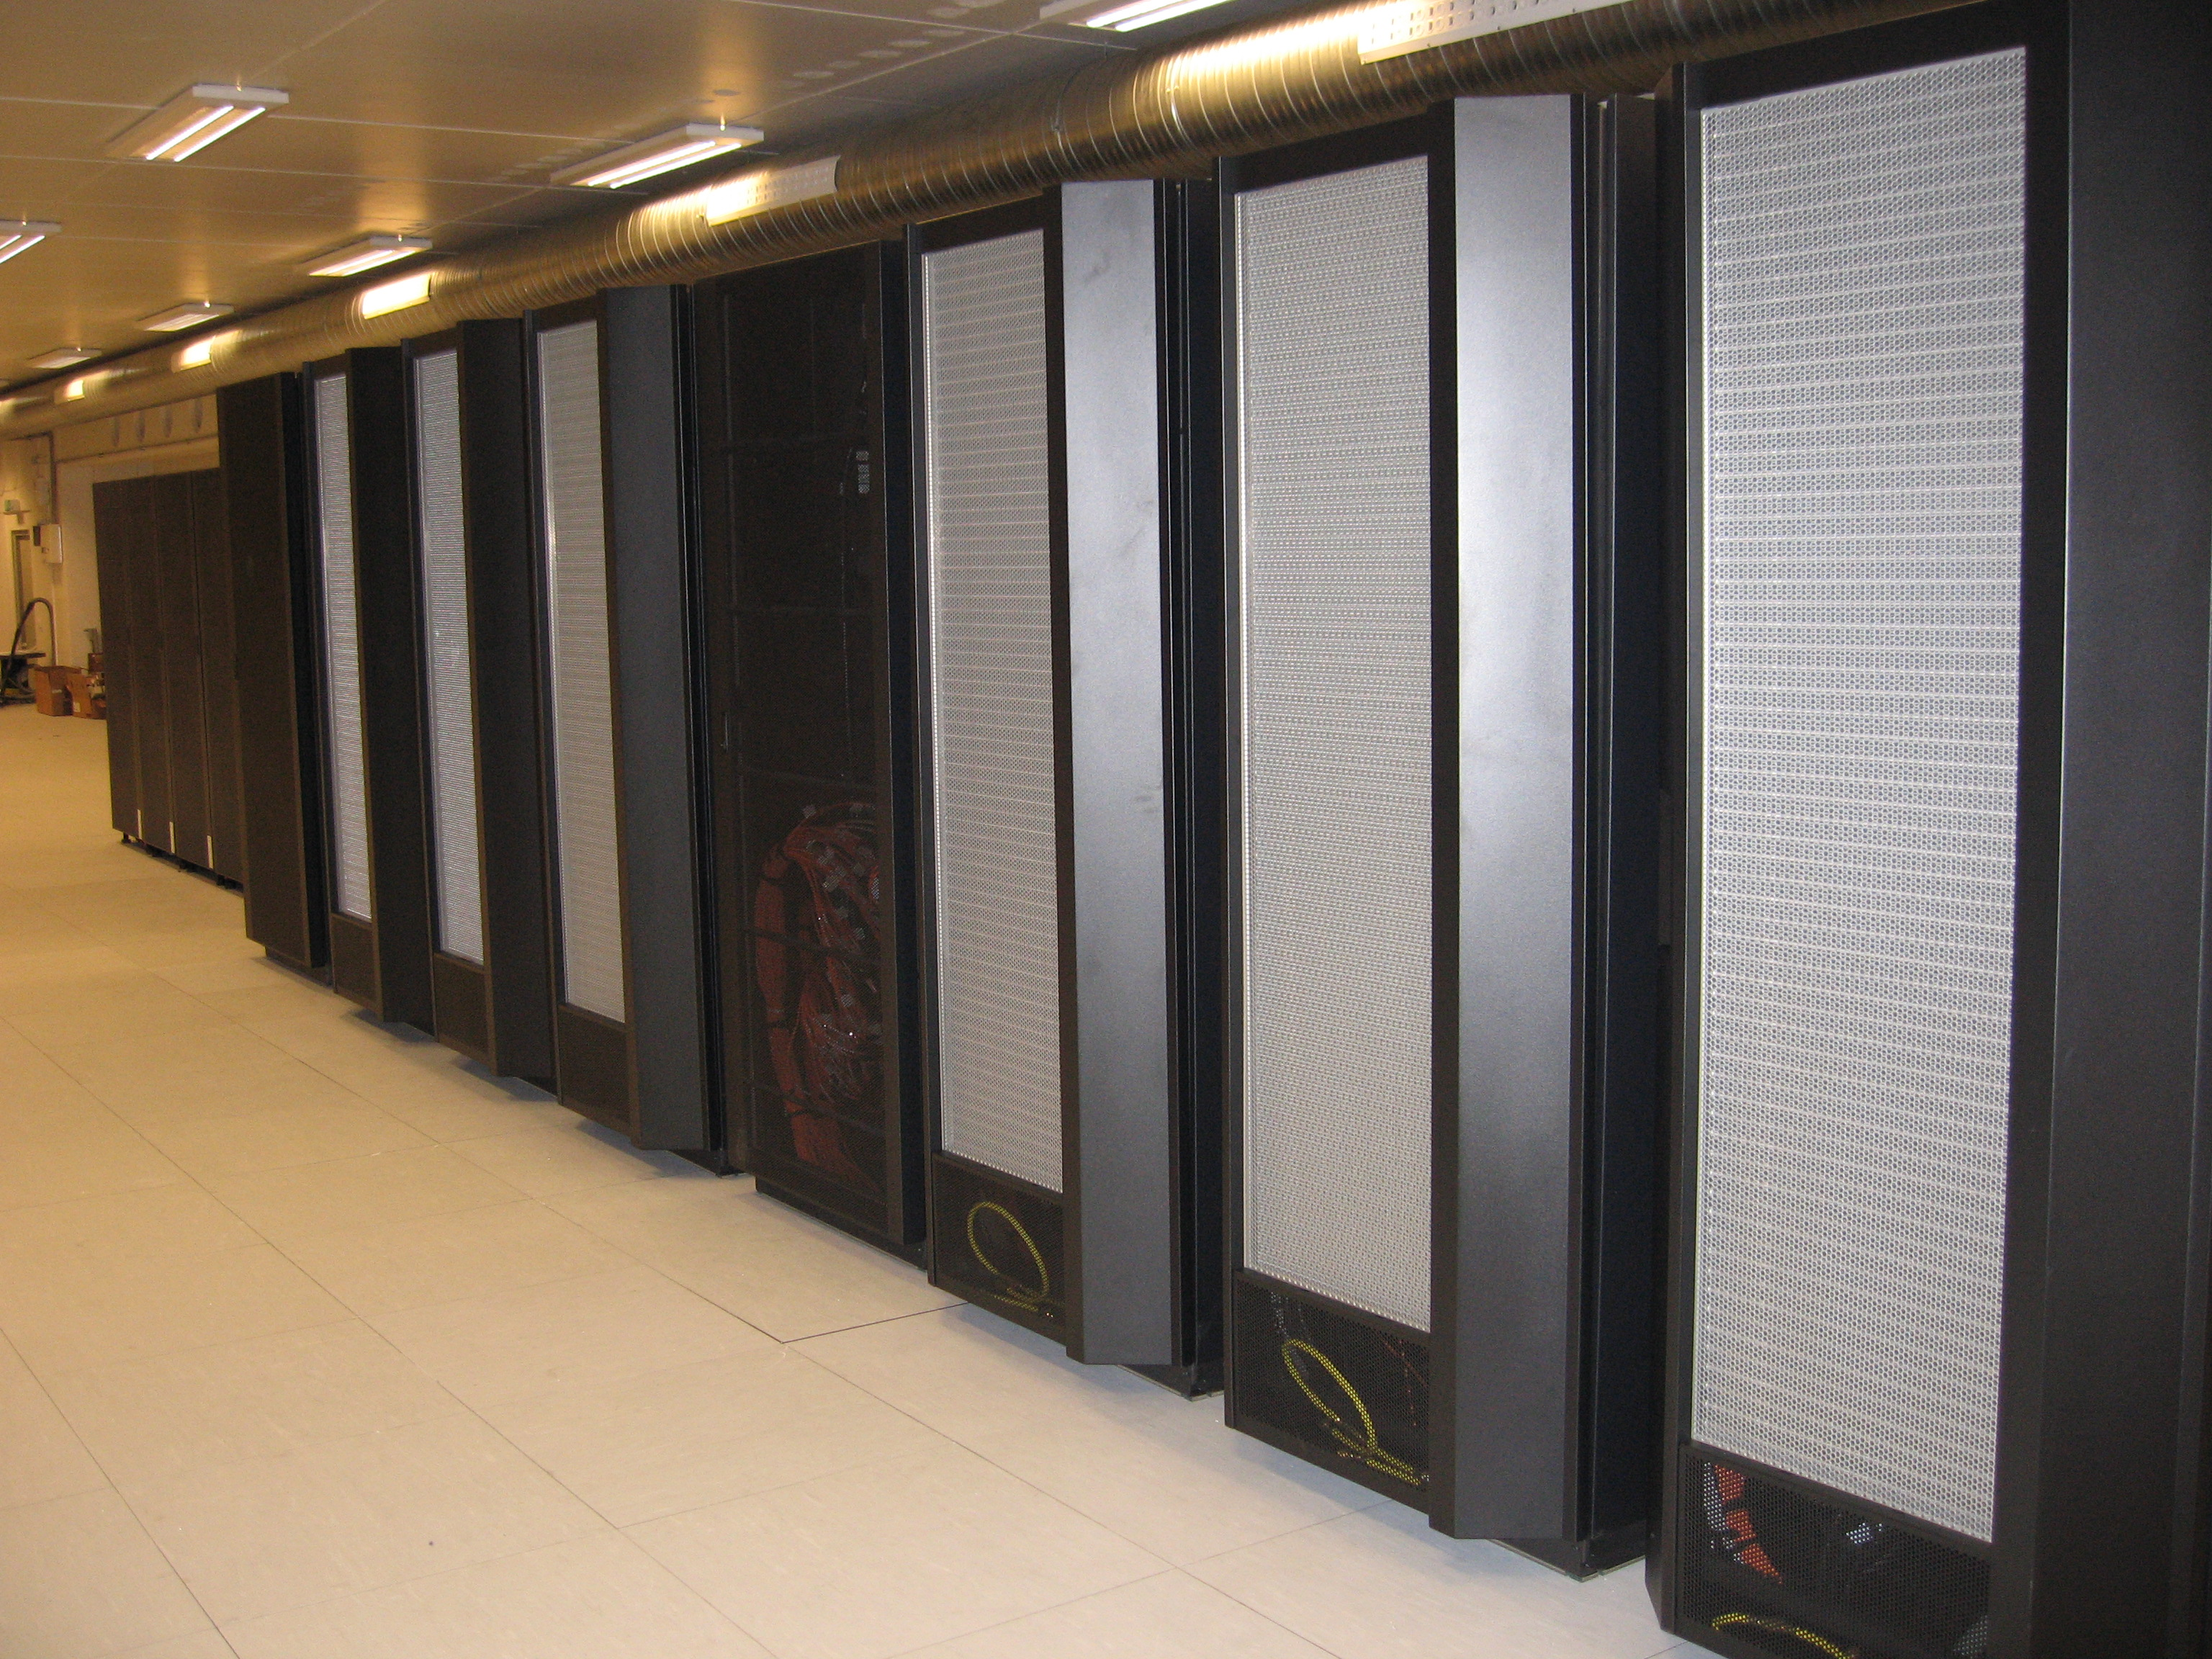
\includegraphics[width=0.6\textwidth]{njord_2}
  \caption{
    \emph{Njord}, the previous IBM supercomputer system at NTNU. Courtesy of
    Arve Dispen.
  }
  \label{fig:njord}
\end{figure}

\begin{figure}
  \centering
  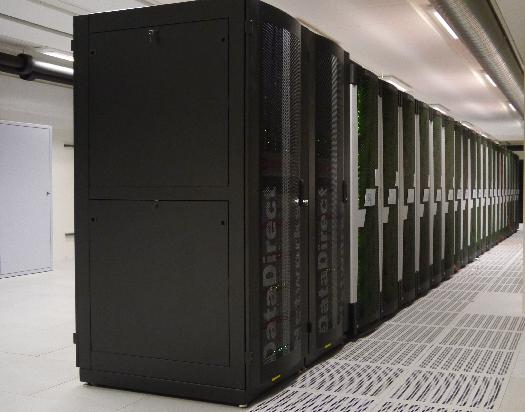
\includegraphics[width=0.6\textwidth]{vilje}
  \caption{
    Photo of \emph{Vilje}, the current SGI supercomputer at NTNU.
    Source: NTNU HPC Wiki.
  }
  \label{fig:njord}
\end{figure}

\section{Applications}

Some sample applications for supercomputing are given in \Autoref{fig:met,
fig:climate}.

\vspace{2cm}
\begin{figure}[!ht]
  \centering
  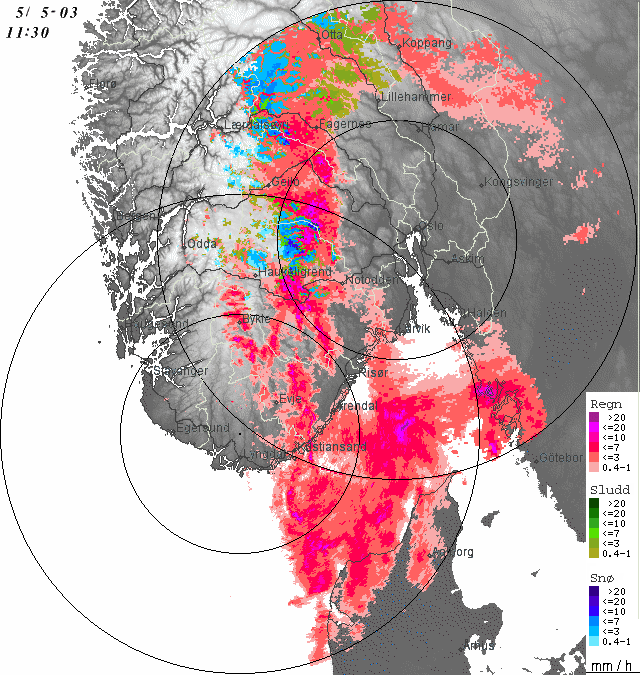
\includegraphics[height=0.6\textheight]{met}
  \caption{
    Example of use of supercomputing: weather forecasting. The Meteorological
    Institute in Norway uses the supercomputer \emph{Njord} every day. Source:
    \protect\url{http://met.no}.
  }
  \label{fig:met}
\end{figure}

\begin{figure}[!ht]
  \centering
  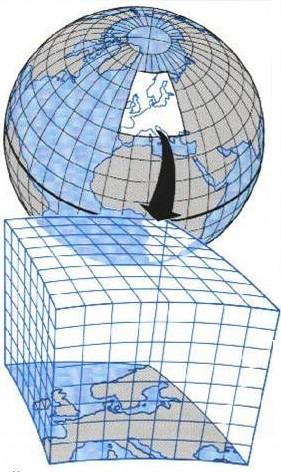
\includegraphics[height=0.6\textheight]{climate_model}
  \caption{
    Example of use of supercomputing: climate modelling. For more information,
    see \protect\url{http://bjerknes.uib.no} (Bjerknes Centre for Climate Research).
  }
  \label{fig:climate}
\end{figure}

\chapter{Single processor systems}

\section{A prototypical processor}

We start by explaining some of the basic tasks performed by a single processor.
The comments are particularly relevant for the MIPS R14000 processor used in a
previous supercomputer at NTNU (called \emph{Gridur}, a SGI Origin 3000 system
used in the period 2001--2007). The MIPS processor is an example of a processor
implementing a RISC architecture (RISC---\emph{Reduced Instruction Set
Computer}), which has been a very important processor design over the past
couple of decades. We will later return to comment on the POWER5 processor
used in the previous supercomputer at NTNU, in particular some of the key
differences compared to the processor discussed in this section. The name POWER
refers to {\em Performance Optimization With Enhanced RISC}, and is also the
name of a series of microprocessors designed by IBM.

\begin{figure}[htbp]
  \centering
  \begin{tikzpicture}[
    block/.style={
      draw=darkblue,
      fill=cadet,
      shape=rectangle,
      rounded corners=1mm,
      text height=1.5ex,
      text depth=.25ex,
    },
    l1/.style={
      minimum height=8mm,
      minimum width=4cm,
    },
    ops/.style={
      minimum height=8mm,
      minimum width=4cm,
      align=right,
    },
    inst/.style={
      minimum height=28mm,
      minimum width=16mm,
    },
    line/.style={
      thick,
      draw=darkblue,
    }]
    \node[block, l1] (L1inst) {L1 Instruction Cache};
    \node[block, l1, right=15mm of L1inst] (L1data) {L1 Data Cache};
    \node[block, l1, above=8mm of L1inst, fill=salmon] (Rest) {RAM, disk, network};
    \node[block, l1, above=8mm of L1data, fill=salmon] (L2) {L2 cache};
    \node[block, ops, below=16mm of L1data.east, anchor=east] (LS) {Load and store};
    \node[block, ops, below=10mm of LS.east, anchor=east] (Int) {Integer};
    \node[block, ops, below=10mm of Int.east, anchor=east] (Float) {Floating point};
    \node[block, inst, below=26mm of L1inst.east, anchor=east] (Decode) {Decode};
    \node[block, inst, below=26mm of L1inst.west, anchor=west] (Branch) {Branch};
    \node[block, inst, below=2mm of Decode, minimum height=8mm] (Clock) {Clock};

    \draw[line, <->] (Rest.east) -- (L2.west);
    \draw[line, <->] (L1inst.east) -- (L1data.west);
    \draw[line, <->] (L1data.south) -- (LS.north);
    \draw[line, ->] (Decode.east) -- (Int.west);
    \draw[line, ->] ([yshift=10mm]Decode.east) -- (LS.west);
    \draw[line, ->] ([yshift=-10mm]Decode.east) -- (Float.west);
    \draw[line, ->] (Decode.west) -- (Branch.east);
    \draw[line, ->] ([xshift=12mm]L1inst.south) -- (Decode.north);
    \draw[line, <-] ([xshift=-12mm]L1inst.south) -- (Branch.north);
    \draw[line] ($(L1inst.east)!0.5!(L1data.west)$) -- ($(Rest.east)!0.5!(L2.west)$);
  \end{tikzpicture}
  \caption{
    A prototypical processor, including the MIPS R14000 used in \emph{Gridur},
    the supercomputer at NTNU during the period 2001--2007. The red components
    are off-chip.
  }
  \label{fig:Lande}
\end{figure}

In order to introduce some key concepts in the RISC architecture, let us briefly
explain what happens when we perform the following simple operation
\begin{align}
  c = a + b.
  \label{single:add1}
\end{align}
Here, we want the processor to add the two numbers $a$ and $b$ and store the
answer in $c$. In this case, $a$ and $b$ are referred to as \emph{operands},
while $+$ is the \emph{operator}. Hence, the simple addition of two scalars
implies a single floating point operation.

The basic unit of ``time'' for our processor is a clock cycle. The state of the
processor changes from clock cycle to clock cycle, depending on what needs to be
done. Different parts/units of the processor work on different tasks
independently of each other. These tasks may correspond to different
instructions, each in a particular phase of completion.

Consider again the addition of two scalars. The operation \eqref{single:add1}
may be part of a larger program involving many operations (or instructions). Let
us assume that the instruction for the ``add'' operation is currently in a small
memory module denoted as L1 cache (for instructions). When the execution of our
program is ready to perform this operation, the instruction is brought into a
decoder and made ready for execution. The addresses of the operands ($a$ and
$b$) are computed and the operands are brought into two registers of the
processors. We assume that the operands are available in the small memory module
called L1 cache (for data).

The operands are then directed from the two registers to the floating point unit
for addition (denoted as FPAdd) where the two numbers are added together. The
whole operation takes just a few clock cycles. For the MIPS R14000 processor,
this operation takes five clock cycles:
\begin{enumerate}
\item read from register
\item align
\item add
\item pack
\item write to register
\end{enumerate}
Note that the number of clock cycles required to perform this operation is not
the same as the number of bits used to store our operands (e.g., 64 bits in
double precision). The reason is that the data flow in the processor happens
along a ``wide bus'' capable of moving all the bits at the same time. This is an
example of bit-level parallelism. Older processors could only move 4, 8, 16, and
32 bits at a time and an add operation therefore took additional clock cycles to
complete. In addition, current processors have a much higher clock frequency (or
shorter clock period) compared to older processors.

Let us now make a few more remarks regarding the processor in
\autoref{fig:Lande}. We have already mentioned the floating point unit for
addition, FPAdd. However, the processor has also other functional units. For
example, the R14000 prosessor has five functional units which can operate
independently from each other:
\begin{itemize}
\item Load/Store: computes memory addresses and to bring operands to and from
the memory;
\item ALU1: a unit for addition and subtraction of integers, and logical
operations;
\item ALU2: a unit for addition, subtraction, multiplication, and division of
integers, as well as logical operations;
\item FPAdd: adds of floating point numbers;
\item FPMult: a unit for multiplication, division, and square root of floating
point numbers.
\end{itemize}
Note that the operands used in these functional units need to come from the
registers in the processor. If the operands are not in the registers, they have
to be brought from the memory into the registers with a {\em load} operation.
The answer (or output) from the functional units are also stored in registers
and subsequently stored in the memory with a {\em store} operation.

\section{Memory hierarchy}

The example from the previous section involving the addition of two floating
point numbers assumed that the instruction for the operation \eqref{single:add1}
was in the memory module denoted as L1 cache for instructions; see
\autoref{fig:Lande}. Similarly, we assumed that the operands $a$ and $b$ were
available in the memory module denoted as L1 cache for data.

Let us now comment a bit more on what happens if these assumptions are not true.
In this case, the program will check whether the instruction or data are
available in the memory module denoted as L2 cache in Figure \ref{fig:Lande}.
This is a memory module which is larger than L1 cache. Furthermore, the L2 cache
is not split into a separate module for instructions and a separate module for
data. It also takes longer (meaning more clock cycles) to fetch data from L2
cache compared to L1 cache. It could also happen that the instruction and the
data the program is looking for is not available in L2 cache either. In this
case data has to be brought in from main memory (RAM) or perhaps even further
away (e.g. the local disk).

Bringing instructions and data to and from memory (from cache, RAM, etc.) is
typically a bottleneck in scientific computing. The processors are getting
faster and faster, but the memory bandwidth (or transfer rate in bytes per
second) is not keeping up at a similar speed. Hence, for certain operations, the
processor can become ``starved'' for data, meaning that it is idle for much of
the time while waiting for data to be transferred to and from memory. The
overall performance in terms of floating point operations per second will in
such cases not be governed by the processor speed, but by the memory access
time.

In order to ``hide'' this difference in speed (i.e., processor speed versus
memory access speed), the memory is organized in a hierarchical fashion;
see \autoref{fig:MemoryHierarchy}.
\begin{figure}
  \centering
  \begin{tikzpicture}[
    line/.style={
      thick,
      draw=darkblue,
    }]
    \coordinate (A) at (-4.5,0) {};
    \coordinate (B) at (4.5,0) {};
    \coordinate (C) at (0,7.4) {};
    \fill[cadet] (A) -- (B) -- (C);
    \draw[line, name path=AC] (A) -- (C);
    \draw[line, name path=BC] (B) -- (C);
    \foreach \y/\A in
    {0/Tape, 1/Distributed memory, 2/Local disk, 3/Main memory (RAM), 4/Cache, 5/Registers, 6/CPU}
    {
      \path[name path=horiz] (A|-0,\y) -- (B|-0,\y);
      \draw[line, name intersections={of=AC and horiz,by=P},
      name intersections={of=BC and horiz,by=Q}] (P) -- (Q)
      node[midway, above=1mm, text height=1.5ex, text depth=.25ex] {\A};
    }
  \end{tikzpicture}
  \caption{
    The memory hierarchy of a computer system. Higher entries are faster, while
    lower entries are cheaper and larger.
  }
  \label{fig:MemoryHierarchy}
\end{figure}
The fastest part of the memory is closest to the CPU. For example, on the MIPS
R14000, the L1 cache is on the chip. This part of the memory is fast, but also
small because it is very expensive. In contrast, the main memory is much larger,
but has also a much longer access time; see \autoref{tbl:cycles}. We will later
discuss in more detail how it is decided what should be in the L1 and L2 cache.

\begin{table}
  \centering
  \caption{
    Typical memory access times for R14000. The numbers represent number of
    clock cycles.
  }
  \label{tbl:cycles}
  \bgroup\def\arraystretch{1.2}
  \begin{tabular}{rl}
    \hline
    Memory type & Clock cycles \\ \hhline{==}
    Registers & $1$ \\ \hline
    L1 cache & $2$--$3$ \\ \hline
    L2 cache & $10$--$12$ \\ \hline
    Main memory &  $100$--$200$ \\ \hline
    Message passing & $\mathcal{O}(10^3)$--$\mathcal{O}(10^4)$ \\ \hline
    Local disk & $\mathcal{O}(10^6)$ \\ \hline
  \end{tabular}
  \egroup
\end{table}

We remark that message passing in \autoref{tbl:cycles} refers to communication
between individual processors by sending messages over a network; we will return
to a discussion of multiple processors later.

\section{Pipelining/vectorization}

Assume now that, instead of (\ref{single:add1}), we would like to add the two
vectors $\bm a$ and $\bm b$ of length $n$ and store the result in a vector $\bm
c$, i.e.
\begin{align}
  \bm c = \bm a + \bm b.
  \label{single:addn}
\end{align}
We can also write \eqref{single:addn} as the loop (in Fortran)
\begin{lstlisting}[style=fortran]
  for i=1,n
    c(i) = a(i) + b(i)
  end
\end{lstlisting}
Again, we start by assuming that the data are available in the registers. From
there, the individual vector elements $a(i)$ and $b(i)$ enter the floating point
unit FPAdd where the numbers are added to produce the output elements $c(i)$,
$i=1,\ldots,n$.

We mentioned earlier that it takes five clock cycles to add two floating point
numbers together. This would perhaps suggest that the total number of clock
cycles for the operation \eqref{single:addn} is $5n$, and that the total
execution time therefore is $5n\tau$ where $\tau$ is the clock period. However,
if things are done optimally, the total number of clock cycles can be reduced to
approximately $n$ for $n\gg 1$. The reason for this is that the five stages in
the adder correspond to independent tasks. This means that, as soon as the
addition of two operands (i.e. $a(i)$ and $b(i)$) has finished the first stage,
two new operands ($a(i+1)$ and $b(i+1)$) can enter the first stage in the adder.
Hence, after five clock cycles, the first number $c(1)$ in the operation
\eqref{single:addn} is ready, while the numbers $c(2)$, $c(3)$, $c(4)$, $c(5)$,
and $c(6)$ are in different phases of completion in the adder.

In summary, after a few clock cycles to ``fill up'' the adder, a new answer
$c(i), i=2,\ldots,n$ is ready every clock cycle. This is what is referred to as
\emph{pipelining} (or sometimes \emph{vectorization}). The reason behind this
term is quite obvious: we constantly feed the floating point unit (in this case,
the adder) so that the ``pipeline'' is always full. In other words, we do not
wait until one answer is ready before we start the process of adding two new
numbers. In this way, we achieve a certain level of parallelism in the sense
that asymptotically (for long vector lengths), the adder works simultaneously on
five different pairs of operands.

The above discussion assumed that the data (i.e. the operands $a(i)$ and $b(i)$,
$i=1,\ldots,n$) are ready for the adder with no delay. Whether this is possible
or not depends on the particular processor. In the case of the MIPS R14000
processor it is not possible to achieve this performance. The reason is that,
in the best case, only a single floating point number can be brought between the
memory (L1 cache) and a register at a time. Since we need to fetch two operands,
$a(i)$ and $b(i)$, per floating point operation, and store the answer $c(i)$
back to memory, a minimum of three clock cycles are needed for memory transfer
per addition. Hence, even though the floating point unit (the adder) can
theoretically complete one addition per clock cycle, the memory traffic will be
the bottleneck, at least for large $n$.

The only possibility for achieving a better performance is if all the operands
are already available in the processors registers. However, since a processor
only has a limited number of registers (on the MIPS R14000 the number of
registers is 64), such performance cannot be acheived if $n \gg 1$.

Let us now predict the optimal performance for the operation \eqref{single:addn}
in the case $n \gg 1$ on Gridur. The clock cycle for each processor is 500 MHz.
Hence, the clock period is 2 ns. Since each floating point operation will
asymptotically require three clock cycles due to the fetch and store operations
(see the discussion above), each floating point operation will at least require
three clock cycles, or 6 ns. Hence, the maximum performance for the operation
\eqref{single:addn} is $(6\cdot 10^{-9})^{-1}$ floating point operations per
second, or approximately 167 MFlops. In practice, less performance may be
achieved, in particular if the operands need to first be brought in from deeper
layers of the memory hierarchy; see \autoref{fig:MemoryHierarchy}.

\section{Superscalar operations}

Consider now a modification of the operation \eqref{single:addn} to the
following operation:
\begin{align}
  \bm c = \bm a + \gamma \bm b.
  \label{single:addmultn}
\end{align}
Here, each vector element $b(i)$, $i=1,\ldots,n$ is multiplied with a scalar,
$\gamma$, before being added to $a(i)$. Similar to the operation
\eqref{single:addn} the result of each addition is stored as the vector element
$c(i)$.

The new operation here is the multiplication. As mentioned earlier, each R14000
processor has a separate floating point unit for multiplication, FPMult. Similar
to the add operation, multiplying two numbers also take five clock cycles:
\begin{enumerate}
\item read from register
\item multiply
\item sum product
\item pack
\item write to register
\end{enumerate}
Hence, all the comments made in the previous section for the operation
\eqref{single:addn} also apply if the add operation $+$ is replaced by
multiplication $\times$.

Let us now comment on what happens when we combine both multiplication and
addition as in \eqref{single:addmultn}. Again, let us first assume that all the
data are readily available (i.e. stored in the registers). The vector elements
$b(i)$ are brought to the multiplier where each element is multiplied by the
scalar $\gamma$; see Figure \autoref{fig:SuperScalar}. After a startup time of
five clock cycles, a new answer is coming out from the multiplier every clock
cycle. We assume here that the pipelining feature is exploited.

\begin{figure}[htbp]
  \centering
  % \begin{center}
  %   \includegraphics[scale=0.9]{SuperScalar}
  % \end{center}
  \begin{tikzpicture}[
    block/.style={
      draw=darkblue,
      fill=cadet,
      shape=rectangle,
      rounded corners=1mm,
      minimum height=12mm,
      minimum width=12mm,
    },
    pinin/.style={pin edge={to-, thick, darkblue}},
    pinout/.style={pin edge={-to, thick, darkblue}},
    ]
    \node[block, pin={[pinin]above:$\gamma$}, pin={[pinin]left:$b(i)$}] (mult) {$\times$};
    \node[block, right=20mm of mult, pin={[pinin]above:$a(i)$}, pin={[pinout]right:$c(i)$}] (add) {$+$};
    \draw[darkblue, ->, thick] (mult.east) -- (add.west);
  \end{tikzpicture}
  \caption{The superscalar operation multiply and add.}
  \label{fig:SuperScalar}
\end{figure}

Each output from the multiplier is now channeled directly as an input to the
adder where it is added to the vector element $a(i)$. After another five clock
cycles, the answer $c(i)$ is ready. Hence, after a startup time of 10 clock
cycles (5 for the multiplier and 5 for the adder), we get one complete answer
$c(i), \, i=1,\ldots,n$ as output every clock cycle. Asymptotically (i.e., for
large vector lengths), the theoretical performance is therefore two floating
point operations per clock cycle. This way of piping the output from one
floating point unit into the input for another unit is denoted as
\emph{superscalar} capability. Similar to the pipelining feature of the adder
and the multiplier, the superscalar capability offers yet another possibility of
parallelism in the sense that each single processor is capable of performing
addition and multiplication at the same time (for sufficiently long vector
lengths).

In practice, the processor has only a limited number of registers, and we need
to fetch the operands from memory (L1 cache) and store the answers in memory.
Similar to the operation \eqref{single:addn}, each complete vector element
$c(i)$ will require three clock cycles due to the memory traffic. However, in
contrast to the operation \eqref{single:addn}, the operation
\eqref{single:addmultn} implies two floating point operations instead of one for
each complete vector element $c(i)$. The maximum single-process performance we
can obtain on R14000 for \eqref{single:addmultn} is thus twice the performance
for \eqref{single:addn}, i.e. 333 MFLOPS.

\section{Cache}

Let us now discuss in more detail the interaction between the cache and the main
memory. The main purpose of the cache is to keep copies of data in extra (and
fast) memory close to the CPU in order to ``hide'' the relatively slow transfer
rate between the main memory and the processor.

Because fast caches are expensive, they tend to be small. As an example, we give
the memory sizes for the R14000 processors. On Gridur, four individual
processors shared up to 4 Gbytes of main memory. Each processor had an L2 cache
of size 8 Mbytes and two L1 caches (one for instructions and one for data), each
only of size 32 Kbytes. Hence, the L1 cache for data can only hold up to 4000
floating point numbers (assuming double precision), which is relatively small in
the context of simulating systems with thousands or millions of unknowns (e.g.,
for the numerical solution of partial differential equations). The L2 cache can
hold more data, but the transfer rate is a little bit longer compared to the L1
cache; see \autoref{tbl:cycles}.

The cache is smaller than the main memory by some power of two. Hence, a
strategy for mapping memory locations to cache locations needs to be defined. We
describe three strategies for doing this.

\subsection{Direct mapped cache}

One strategy is to use what is refered to as a \emph{direct mapped cache}. In
this case, each location in main memory corresponds to a unique location in
cache; see \autoref{fig:DirectMappedCache}. The main memory address is split
into two parts: the first bits of the memory address are called the \emph{set
bits} and these bits give the precise cache address. The remaining bits are
called the \emph{tag bigs}, and these are used to determine if a copy of the
content at the particular main memory location has been copied into the cache
location given by the set bits. With this strategy we see that several main
memory addresses map to the same cache address.
\[
  \text{Memory address} =
  \underbrace{b_1 \ldots b_k}_{\text{tag bits}}
  \underbrace{b_{k+1} \ldots b_{N}}_{\text{cache address}}.
\]

\begin{figure}
  \centering
  \begin{tikzpicture}[scale=0.3]
    \def \n {7};
    \def \k {3};
    \def \q {1};
    \def \s {3};

    \foreach \i [
      evaluate=\i as \R using -(\n+1)*\i,
      evaluate=\i as \L using -(\n+1)*(\i+1),
    ] in {0,...,\k}
    {
      \fill[cadet] (\R-\q, 0) -- (\R-\q, -2) -- (\R-\q-1, -2) -- (\R-\q-1, 0) -- (\R-\q, 0);
      \fill[salmon] (\R-\s, 0) -- (\R-\s, -2) -- (\R-\s-1, -2) -- (\R-\s-1, 0) -- (\R-\s, 0);
      \draw[darkblue, very thick] (\R, 0) -- (\R, -2) -- (\L, -2) -- (\L, 0) -- (\R, 0);
      \foreach \j [
        evaluate=\j as \l using \R-\j
      ] in {1,...,\n}
      {
        \draw[darkblue, very thin] (\l, 0) -- (\l, -2);
      }
    }

    \fill[cadet] (-\q, 3) -- (-\q, 1) -- (-\q-1, 1) -- (-\q-1, 3) -- (-\q, 3);
    \fill[salmon] (-\s, 3) -- (-\s, 1) -- (-\s-1, 1) -- (-\s-1, 3) -- (-\s, 3);
    \draw[darkblue, very thick] (0, 3) -- (0, 1) -- (-\n-1, 1) -- (-\n-1, 3) -- (0, 3);
    \foreach \j in {1,...,\n} {
      \draw[darkblue, very thin] (0-\j, 3) -- (0-\j, 1);
    }

    \node[anchor=west] at (0, -1) {RAM};
    \node[anchor=west] at (0, 2) {Cache};
  \end{tikzpicture}
  \caption{
    A direct mapped cache. Each main memory address maps to a unique and
    pre-determined location in the cache.
  }
  \label{fig:DirectMappedCache}
\end{figure}

When some particular data is requested by the program, e.g., a floating point
number, the processor will check whether the data is stored in L1 cache. It does
this by looking up the cache address (taking the least significant bits of the
memory address) and checking whether the tag bits at that location match the tag
bits of the memory address. If is not in L1 cache, the processor will check
whether the data is stored in L2 cache. If this is the case, the requested data
will be copied from the L2 cache into L1 cache. If the data is not in L2 cache
either, the data will have to be brought in from main memory. In this case, a
copy will be made in L2 cache as well as in L1 cache. In either case, the tag
bits at the given cache address will be updated to match the new mapped
location.

Note that when a floating point number (or an integer) is requested by the
program, more than a single number is copied into cache. The minimum amount of
data copied is called a {\em cache line}. For the R14000 processor, the cache
line for the L1 cache is 32 bytes (corresponding to four floating point numbers
in double precision), while the cache line for the L2 cache is 128 bytes
(corresponding to 16 floating point numbers in double precision). The extra
numbers copied are the numbers in the adjacent memory locations in main memory.

Consider again the operation \eqref{single:addn}. Assume that the vectors $\bm
a$, $\bm b$ and $\bm c$ represent floating point numbers in double precision,
and that the vectors are stored after each other in main memory. Let the vector
length $n=4000$, i.e. each vector will precisely fill the L1 data cache. For
every element $c(i)$ computed, the operands $a(i)$ and $b(i)$ will need to be
brought in all the way from main memory due to the fact that $a(i)$, $b(i)$ and
$c(i)$ happen to have the same cache address. A severe drop in performance will
be observed in this case. This situation is refered to as cache trashing; see
\autoref{fig:CacheTrashing}.

\begin{figure}
  \centering
  \begin{tikzpicture}[scale=0.3]
    \def \n {7};
    \def \k {3};
    \def \q {1};

    \foreach \i [
      evaluate=\i as \R using -(\n+1)*\i,
      evaluate=\i as \L using -(\n+1)*(\i+1),
    ] in {0,...,\k}
    {
      \fill[cadet] (\R-\q, 0) -- (\R-\q, -2) -- (\R-\q-1, -2) -- (\R-\q-1, 0) -- (\R-\q, 0);
      \draw[darkblue, very thick] (\R, 0) -- (\R, -2) -- (\L, -2) -- (\L, 0) -- (\R, 0);
      \foreach \j [
        evaluate=\j as \l using \R-\j
      ] in {1,...,\n}
      {
        \draw[darkblue, very thin] (\l, 0) -- (\l, -2);
      }
    }

    \fill[cadet] (-\q, 3) -- (-\q, 1) -- (-\q-1, 1) -- (-\q-1, 3) -- (-\q, 3);
    \draw[darkblue, very thick] (0, 3) -- (0, 1) -- (-\n-1, 1) -- (-\n-1, 3) -- (0, 3);
    \foreach \j in {1,...,\n} {
      \draw[darkblue, very thin] (0-\j, 3) -- (0-\j, 1);
    }

    \node[anchor=west] at (0, -1) {RAM};
    \node[anchor=west] at (0, 2) {Cache};
    \node[anchor=north] at (-\q-0.5, -2) {\scriptsize $a(i)$};
    \node[anchor=north] at (-\n-1-\q-0.5, -2) {\scriptsize $b(i)$};
    \node[anchor=north] at (-\n-\n-2-\q-0.5, -2) {\scriptsize $c(i)$};
    \node[anchor=south] at (-\q-0.5, 3) {\scriptsize ??};
  \end{tikzpicture}
  \caption{
    Cache trashing. The corresponding elements in the vectors $\bm a$, $\bm b$
    and $\bm c$ all map to the same cache address.
  }
  \label{fig:CacheTrashing}
\end{figure}

Cache trashing can be avoided by storing the elements in the vectors $\bm a$,
$\bm b$ and $\bm c$ in a different way; see Figure \ref{fig:AdjacentMemory}. We
remark that the crash trashing example given here is perhaps not likely to
happen. Nonetheless, it illustrates the point that severe performance
degradation is possible to observe due to undesirable memory traffic.

\begin{figure}
  \centering
  \begin{tikzpicture}[
    scale=0.8,
    every node/.style={
      text height=1.5ex,
      text depth=.25ex,
    }
    ]
    \draw[darkblue, very thick] (-6, 0) -- (6, 0);
    \draw[darkblue, very thick] (-6, 1) -- (6, 1);
    \draw[darkblue, very thin] (-3, 0) -- (-3, 1);
    \draw[darkblue, very thin] (-2, 0) -- (-2, 1);
    \draw[darkblue, very thin] (-1, 0) -- (-1, 1);
    \draw[darkblue, very thin] (0, 0) -- (0, 1);
    \draw[darkblue, very thin] (1, 0) -- (1, 1);
    \draw[darkblue, very thin] (2, 0) -- (2, 1);
    \draw[darkblue, very thin] (3, 0) -- (3, 1);
    \node at (-3.5, 0.5) {\footnotesize $\cdots$};
    \node at (-2.5, 0.5) {\footnotesize $a_i$};
    \node at (-1.5, 0.5) {\footnotesize $b_i$};
    \node at (-0.5, 0.5) {\footnotesize $c_i$};
    \node at (0.5, 0.5) {\footnotesize $a_{i+1}$};
    \node at (1.5, 0.5) {\footnotesize $b_{i+1}$};
    \node at (2.5, 0.5) {\footnotesize $c_{i+1}$};
    \node at (3.5, 0.5) {\footnotesize $\cdots$};
  \end{tikzpicture}
  \caption{Adjacent memory layout.}
  \label{fig:AdjacentMemory}
\end{figure}

\subsection{Fully associative cache}

To avoid the possibility of cache trashing, we can use a different cache
strategy called a \emph{fully associative cache}. In a fully associative cache,
each cache address can map to any memory address. This is essentially a direct
mapped cache where all the bits are used as tag bits and no bits are used as a
cache address.

To find the corresponding cache location for a given memory address, the tag
bits of all cache locations must be checked. This is typically done in parallel
using dedicated hardware, which is rather complicated. For this reason, fully
associative caches are rarely seen.

When the cache is full, a cache line must be evicted to make way for new data.
How this happens depends on the replacement policy:
\begin{itemize}
\item Least recently used (LRU);
\item Least frequently used (LFU);
\item Random
\end{itemize}
In the context of numerical solution of partial differential equations, the
alternative \emph{LRU} generally gives the best performance. This can be
understood by the fact that such problems typically exhibit significant locality
in time and space: data that has recently been used has a high chance of being
used again in the near future; and data close (in space) to recently used data
has a high chance of being used in the near future.

\subsection{Set-associative cache}

A \emph{set-associative} cache is a nice compromise between a direct mapped
cache and a fully associative cache. In a set-associative cache, the cache is
split into chunks of $n$ cache lines. Each memory address maps deterministically
to a given chunk (according to its least significant bits) precisely as a direct
mapped cache. However, within this chunk the mapping proceeds as with a fully
associative cache with $n$ choices.

The cache eviction strategies work the same way as for a fully associative
cache.

\chapter{Introduction to git}

The scope of this chapter is to explain the basic mechanisms of git. Git is a
complex tool, using it to its full power can take quite some time to learn.
Something crucial may have been missed while attempting to boil it down to
basics. There is a whole internet full of guides out there and you are
encouraged to supplement these ramblings with more verbose tutorials and
articles. Also, please do not hesitate to ask during lectures or breaks; I love
it when people talk git to me.

\section{Installing git}

Start by installing git on your laptop; on Ubuntu you can do this through
\begin{lstlisting}[style=shell]
  sudo apt-get install git
\end{lstlisting}

\section{Setting up a GIT repository}

You can set up a GIT directory in two ways. You either clone a remote repository
or initialize a new, empty one. In either case you end up on a \emph{branch}
called \emph{master} by default.

To clone a remote repository do
\begin{lstlisting}[style=shell]
  git clone <url>
\end{lstlisting}
where \texttt{<url>} is the URL of the repository to clone. E.g.
\begin{lstlisting}[style=shell]
  git clone /some/path/on/my/computer
  git clone https://github.com/TheBB/TMA4280
\end{lstlisting}
To initialize an empty repository, change to the directory you would like to use
and do
\begin{lstlisting}[style=shell]
  git init .
\end{lstlisting}

\section{Layout of a git repository}

A repository has two parts; the repository information and your local working
tree. The first contains information about all the individual commits, commit
messages, and branches (a sequence of commits) that is recorded. This is stored
in a folder called \texttt{.git} in the root of the repository. The second part
is your local copy of the files in the repository.

You can make a \emph{bare} clone of a repository. This is a directory that only
contains the repository information, i.e. only the \emph{.git} folder of a
normal clone, and no local working tree. You do this through
\begin{lstlisting}[style=shell]
  git clone --bare <url>
  git init --bare .
\end{lstlisting}

As far as git is concerned, adding files already existing locally is handled as
a change to the file where everything was changed (see further down). You just
want to add source code, not files generated by the build system or the compiler
such as object files, libraries, executables or scripts.

\section{Keeping track of changes}

You can see what changes you have made to your local working directory through
\begin{lstlisting}[style=shell]
  git diff
\end{lstlisting}
If you just want to see which files, are changed, but not the changes
themselves, you can use
\begin{lstlisting}[style=shell]
  git status
\end{lstlisting}
This is in general quite useful, it can show more things such as which changes
are marked for committing.

To mark some changes for committing, do
\begin{lstlisting}[style=shell]
  git add <file>
\end{lstlisting}
This \emph{stages} the changes, but they have not yet been committed. To commit
all staged changes, use
\begin{lstlisting}[style=shell]
  git commit
\end{lstlisting}
This will open a text editor where you can enter a commit message. You can
control \emph{which} editor by adding a line such as
\begin{lstlisting}[style=shell]
  export EDITOR=<myeditor>
\end{lstlisting}
to your \texttt{\textasciitilde/.bashrc} file if you are using bash.
Alternatively, you can specify the commit message directly.
\begin{lstlisting}[style=shell]
  git commit -m "my message"
\end{lstlisting}
You can quickly commit all changes (even unstaged ones) to all tracked files by
doing
\begin{lstlisting}[style=shell]
  git commit -a
\end{lstlisting}
The two can be combined:
\begin{lstlisting}[style=shell]
  git commit -am "my message"
\end{lstlisting}

\section{Keeping track of commits}
You can see the commit log through
\begin{lstlisting}[style=shell]
  git log
\end{lstlisting}
You can see the log of commits through
\begin{lstlisting}[style=shell]
  git show <commit>
\end{lstlisting}
The commit hash can be found using git log. Alternatively, you have a few
shortcuts. If you omit the revision, the last commit in the branch will be
shown. If you want to show the previous commit, you can use
\begin{lstlisting}[style=shell]
  git show HEAD~1
\end{lstlisting}

\section{Working with remote repositories}
A remote repository is a clone of this repository. Since GIT is a distributed
revision control system, you can clone a clone, and it still contains all the
information the original clone had.

To add a new remote repository, use
\begin{lstlisting}[style=shell]
  git remote add <name> <url>
\end{lstlisting}
where \texttt{<name>} is a name you want to give the remote. If you initialize a
repository through cloning another, the repository you cloned will be registered
as a remote named \emph{origin}. If you started from scratch, there will be no
remotes by default.

To send data between remotes you can \emph{push} or \emph{pull}.

To push changes to a remote, use
\begin{lstlisting}[style=shell]
  git push <remote> <branch>
\end{lstlisting}
If you omit the branch name, all branches will be pushed. If changes you have
done conflict with changes done in the remote GIT, your push will be denied. You
then have to \emph{pull} from the remote before you push. A push will also be
denied if you push to a remote with a local working tree, and you try to push to
the branch currently checked out on the remote.

To pull changes from a remote, use
\begin{lstlisting}[style=shell]
  git pull --rebase <remote> <branch>
\end{lstlisting}
If you omit the branch name, all branches will be pulled. Please do not forget
the rebase, or you can get yourself in trouble. The pull model is more involved
to explain, and deemed outside the scope of this document.

If there are conflicts, git will try to resolve them. If it cannot, you must do
it. To see which files are in conflict you can use \emph{git status}. Where
there were conflicts you will have something that looks like the following:
\begin{lstlisting}
  <<<<<<< HEAD
  line11
  line22
  =======
  line12
  line21
  >>>>>>> 7f8de8cd5f58cd2fa0b2d18f002ce9d9431c0b8c
\end{lstlisting}

The first line is a starting marker. This is followed by lines that are in
conflict, these are from the local repository. After the equal signs follow the
lines in conflict from the remote repository. Finally an ending marker and the
commit hash from the remote. Change it into what you want it to be and save the
file. Remember that there may be multiple blocks in conflict in each file!

Stage the resolved files through \texttt{git add} and continue the rebase by
doing
\begin{lstlisting}
  git rebase --continue
\end{lstlisting}

\chapter{Multiprocessor systems}

\section{Supercomputing}

Supercomputing represents the high performance segment of the overall computing
market. This segment has traditionally been driven by grand challenge problems
in science and engineering. This is still the situation, although new areas and
new applications are constantly being added to the list of problems where
supercomputing is necessary (or at least highly desirable).

A strong motivation for using supercomputing is the possibility of performing
larger and more realistic simulations, e.g., by solving more detailed
mathematical models in science and engineering. Hence, the design of the largest
computing systems have traditionally be driven by challenges in science and
engineering.

About 30--40 years ago, supercomputers were typically specially designed vector
processors capable of performing operations on vector data. A single instruction
could operate on multiple data elements (vectors) at once, and the hardware
comprised custom-made chips. Because of the low production volume and the costly
development effort, each supercomputer was very expensive.

Supercomputers in the 80s and 90s also used fast, expensive, custom-made chips,
and combined a few of these in a multiprocess context. However, starting in the
late 80s, microprocessor-based supercomputers became more and more popular.
These systems were also called \emph{massively parallel processors} (MPPs)
because they used many more processors than traditional vector supercomputers.
The advantage of the microprocessor-based supercomputers was the use of
standard, off-the-shelf microprocessors instead of using costly, custom-made
chips. The supercomputer market today is dominated by MPP systems. A
supercomputer system typically combines thousands of processors. Some of the
largest systems comprise hundreds of thousands of processors.

Supercomputing is very resource demanding in terms of floating point operations,
memory and storage requirement, as well as visualization capabilities. Thus,
some of the important challenges related to the development and use of a
multiprocessor system concern:
\begin{enumerate}
\item communication between the processors \\
(network topology, memory access, programming models);
\item development of suitable computational methods or algorithms \\
(e.g., domain decomposition algorithms);
\item scalability (both in terms of hardware and algorithms);
\item handling of large volumes of data (storage and visualization).
\end{enumerate}

We add some additional remarks regarding scalability. Let $T_P$ be the time to
solve a given problem on $P$ processors, where time refers to wall clock time.
We define the speedup, $S_P$, as
\begin{align}
  S_P = \frac{T_1}{T_P},
  \label{multi:speedup}
\end{align}
i.e. as the ratio between the solution time on a single processor divided by the
solution time on $P$ processors. Ideally, we would like $S_P$ to be equal to
$P$, implying the $P$ processors should be able to solve the problem $P$ times
as fast as a single processor. A more realistic situation is depicted in
\autoref{fig:scalability}: for small systems (i.e. when $P$ is small), we
typically get good speedup for a fixed problem. As more processors are added,
the computational task per processor is reduced, while the communication
overhead between the processors typically increases. Hence, after a certain
number of processors, it does not pay off to add more processors.

Note that the above situation gives a too pessimistic view of supercomputing.
The assumption about a fixed problem size is typically not correct. With the
availability of larger computing systems, the problem size is typically also
increased. Many problems solved on large systems are of a size that cannot be
solved in a single processor context, either because of the storage requirement,
because of the computational cost, or both. From this view point, the definition
of speedup in \eqref{multi:speedup} must be used with some care.

\begin{figure}
  \centering
  \begin{tikzpicture}
    \begin{axis}[
      xmin=0,
      xmax=1.3,
      ymin=0,
      ymax=1.3,
      axis lines=middle,
      ticks=none,
      xlabel={$P$},
      ylabel={$S_P$},
      ]
      \addplot[dashed, thick, domain=0:1.1, samples=100]{x};
      \addplot[blue, thick, domain=0:1.3, samples=100]{x/(1+x^5)};
      \node at (axis cs:1.0,1.1) [anchor=east] {Ideally};
      \node at (axis cs:1.13,0.3) [anchor=east] {Realistically};
    \end{axis}
  \end{tikzpicture}
  \caption{Ideal speedup ($S_P = P$) and realistic speedup.}
  \label{fig:scalability}
\end{figure}

Finally, a couple of important reminders: when working in a multiprocessor
environment, the single-processor performance is still of utmost importance. In
particular we recall some of the possibilities of parallelism within a single
processor: bit-level, instruction-level, pipelining, and superscalar
capabilities (or multiple floating point units).

\section{Organization of multiprocessor systems}

According to Almasi and Gottlieb (1989), a parallel computer is a collection of
processing elements which communicate and cooperate to solve a problem fast.
This definition raises some immediate questions:
\begin{itemize}
\item How many processing elements should we use?
\item How should the processing elements communicate?
\item Will the parallel computer be scalable?
\item How powerful should a processor be?
\item What about programming?
\end{itemize}

\Autoref{fig:multiprocess1, fig:multiprocess2} show two examples of
organizations. In \autoref{fig:multiprocess1} each processor has a local cache
and can access memory modules via some type of interconnect. In this case, all
the memory modules can be accessed directly by all the processors. This
organization is referred to as \emph{global} or \emph{shared memory access}. In
\autoref{fig:multiprocess2} each processor has local memory and can only access
information in other memory modules via an interconnecting network. This
organization is referred to as \emph{distributed memory access}. Each
organization has its strengths and weaknesses. We will return to some of these
issues later.

\begin{figure}
  \centering
  \begin{tikzpicture}[scale=0.5]
    \foreach \i in {0,4,8}
    {
      \draw[darkblue, fill=cadet, thick] (\i,10) rectangle (\i+2,7);
      \draw[darkblue, very thin, dashed] (\i,8.5) -- (\i+2,8.5);
      \draw[darkblue, fill=cadet, thick] (\i,3) rectangle (\i+2,1.5);
      \draw[darkblue, thick] (\i+1,7) -- (\i+1,6);
      \draw[darkblue, thick] (\i+1,3) -- (\i+1,4);
      \node at (\i+1,9.25) {P};
      \node at (\i+1,7.75) {\$};
      \node at (\i+1,2.25) {M};
    }
    \draw[darkblue, thick] (0,6) rectangle (10,4);
    \node at (5,5) {Interconnect};
  \end{tikzpicture}
  \caption{A parallel computer with global memory access.}
  \label{fig:multiprocess1}
\end{figure}

\begin{figure}
  \centering
  \begin{tikzpicture}[scale=0.5]
    \foreach \i in {0,4,8}
    {
      \draw[darkblue, fill=cadet, thick] (\i,10) rectangle (\i+2,7);
      \draw[darkblue, very thin, dashed] (\i,8.5) -- (\i+2,8.5);
      \draw[darkblue, fill=cadet, thick] (\i,6) rectangle (\i+2,4.5);
      \draw[darkblue, thick] (\i+1,7) -- (\i+1,6);
      \draw[darkblue, thick] (\i+1,3.5) -- (\i+1,4.5);
      \node at (\i+1,9.25) {P};
      \node at (\i+1,7.75) {\$};
      \node at (\i+1,5.25) {M};
    }
    \draw[darkblue, thick] (0,1.5) rectangle (10,3.5);
    \node at (5,2.5) {Interconnect};
  \end{tikzpicture}
  \caption{A parallel computer with distributed memory access.}
  \label{fig:multiprocess2}
\end{figure}

\subsection{Uniform memory access}

There are several ways to achieve global memory access. One type of systems is
referred to as SMP: \emph{Symmetric Multi-Processor}. This is a configuration
where all the memory locations are ``equidistant'' in the sense that the memory
access time is the same.

An example of an SMP is a bus-based organization; see
\autoref{fig:bus_organization}. This system has a broadcast interconnect similar
to ethernet. It is inexpensive and it is easy to add processors. The
disadvantage with a bus organization is the very limited scalability, which is
due to the fact that the aggregate bandwidth is fixed. The use of caches could
potentially alleviate some of this problem, but then the question of how to
achieve cache coherency (or consistency) arises.

\begin{figure}
  \centering
  \begin{tikzpicture}[scale=0.5]
    \foreach \i in {-1,3}
    {
      \draw[darkblue, fill=cadet, thick] (\i,4) rectangle (\i+2,1);
      \draw[darkblue, very thin, dashed] (\i,2.5) -- (\i+2,2.5);
      \draw[darkblue, thick] (\i+1,1) -- (\i+1,0);
      \node at (\i+1,3.25) {P};
      \node at (\i+1,1.75) {\$};
    }
    \foreach \i in {7,11}
    {
      \draw[darkblue, fill=cadet, thick] (\i,2.5) rectangle (\i+2,1);
      \draw[darkblue, thick] (\i+1,1) -- (\i+1,0);
      \node at (\i+1,1.75) {I/O};
    }
    \foreach \i in {1,5,9}
    {
      \draw[darkblue, fill=cadet, thick] (\i,-2.5) rectangle (\i+2,-1);
      \draw[darkblue, thick] (\i+1,-1) -- (\i+1,0);
      \node at (\i+1,-1.75) {M};
    }
    \draw[red, very thick, <->] (-3,0) -- (15,0);
  \end{tikzpicture}
  \caption{
    A bus-based organization. The global memory is accessible to each processor.
  }
  \label{fig:bus_organization}
\end{figure}

Another example of an SMP is a crossbar or a switch-based organization. Similar
to a bus-based system, cache coherency is needed (e.g. via broadcast). A
crossbar has a better scalability than a bus organization. The aggregate
bandwidth is increased, but adding a processor becomes more and more expensive
as the system size grows (because the number of parts increases).

\begin{figure}
  \centering
  \begin{tikzpicture}[scale=0.5]
    \foreach \i in {0,3,6,9}
    {
      \draw[red, very thick] (0,\i) -- (11,\i);
      \draw[red, very thick] (\i,0) -- (\i,11);

      \draw[darkblue, fill=cadet, thick] (11,\i+.75) rectangle (13,\i-.75);
      \node at (12,\i) {M};
    }

    \foreach \i in {0,3}
    {
      \draw[darkblue, fill=cadet, thick] (\i-1,14) rectangle (\i+1,11);
      \draw[darkblue, very thin, dashed] (\i-1,12.5) -- (\i+1,12.5);
      \node at (\i,13.25) {P};
      \node at (\i,11.75) {\$};
    }

    \foreach \i in {6,9}
    {
      \draw[darkblue, fill=cadet, thick] (\i-1,12.5) rectangle (\i+1,11);
      \node at (\i,11.75) {I/O};
    }
  \end{tikzpicture}
  \caption{
    A crossbar interconnect. The global memory is accessible to each processor.
  }
  \label{fig:crossbar}
\end{figure}

In summary, there is a scalability problem with the interconnect both with a bus
organization and with a crossbar. In the case of the bus, the scalability issue
is due to the fixed aggregate bandwidth; in the case of the crossbar, the
scalability relates to the cost. An example of a compromise between these two
issues is the multistage interconnect; see
\autoref{fig:multistage_interconnect}.

\begin{figure}
  \centering
  \begin{tikzpicture}[scale=0.5]
    \foreach \i in {0,4,8,12}
    {
      \draw[darkblue, fill=cadet, thick] (\i-1,0) rectangle (\i+1,1.5);
      \draw[darkblue, thick] (\i,1.5) -- (\i,2.5);
      \draw[darkblue, thick] (\i,8.5) -- (\i,9.5);
      \node at (\i,0.75) {M};
    }

    \foreach \i in {0,4}
    {
      \draw[darkblue, fill=cadet, thick] (\i-1,12.5) rectangle (\i+1,9.5);
      \draw[darkblue, very thin, dashed] (\i-1,11) -- (\i+1,11);
      \node at (\i,11.75) {P};
      \node at (\i,10.25) {\$};
    }

    \foreach \i in {8, 12}
    {
      \draw[darkblue, fill=cadet, thick] (\i-1,9.5) rectangle (\i+1,11);
      \node at (\i,10.25) {I/O};
    }

    \foreach \i in {2, 10}
    {
      \foreach \j in {3.5, 7.5}
      {
        \draw[darkblue, thick] (\i-3,\j-1) rectangle (\i+3,\j+1);
        \node at (\i,\j) {Interconnect};
      }
    }

    \draw[darkblue, thick] (0,4.5) -- (0,6.5);
    \draw[darkblue, thick] (12,4.5) -- (12,6.5);
    \draw[darkblue, thick] (4,4.5) -- (8,6.5);
    \draw[darkblue, thick] (8,4.5) -- (4,6.5);
  \end{tikzpicture}
  \caption{
    A multi-stage interconnect. The global memory is accessible to each processor.
  }
  \label{fig:multistage_interconnect}
\end{figure}

\subsection{Non-uniform memory access}

An alternative to an SMP-organization is a NUMA-organization (\emph{Non-Uniform
Memory Access}); see \autoref{fig:NUMA}. The last supercomputers at NTNU all
represent examples of this type of organization.

\begin{figure}
  \centering
  \begin{tikzpicture}[scale=0.5]
    \foreach \i in {3, 10}
    {
      \draw[darkblue, thick] (\i+1,-2) -- (\i+1,0);
      \draw[darkblue, thick] (\i,-2) -- (\i+2,-2);

      \draw[darkblue, fill=cadet, thick] (\i-2,-2.75) rectangle (\i,-1.25);
      \node at (\i-1,-2) {M};

      \draw[darkblue, fill=cadet, thick] (\i+2,-1.25) rectangle (\i+4,-4.25);
      \draw[darkblue, very thin, dashed] (\i+2,-2.75) -- (\i+4,-2.75);
      \node at (\i+3,-2) {\$};
      \node at (\i+3,-3.5) {P};
    }

    \draw[red, very thick, <->] (0,0) -- (18,0);
    \node[anchor=south] at (9,0) {Scalable network};
    \node[anchor=west] at (15,-2) {$\cdots$};
  \end{tikzpicture}
  \caption{A NUMA organization.}
  \label{fig:NUMA}
\end{figure}

The Cray T3E had caches which were only used to hold data and instructions from
local memory. The computer had no mechanism to keep the caches consistent with
the global address space. The computer was an example of a non-coherent shared
memory machine. In principle, any processor could read/write from/to any memory
location in the global address space. In practice, however, messages were used
to transfer data from one local memory module to another. The programming model
was thus based on message passing. We will return to this model later.

On the SGI Origin, data from any memory location could be replicated into any of
the caches. Hardware support existed to keep the caches consistent. This is also
referred to as a ccNUMA organization (\emph{cache coherent Non-Uniform Memory
Access}). Any processor could read/write from/to any memory location. This
feature could be exploited in a shared memory programming model. However, note
that a message passing programming model could still be used on the SGI. We will
return to a discussion of the current supercomputer at NTNU later.

\subsection{Distributed memory access}

An example of a distributed memory organization is the mesh interconnect as
depicted in \autoref{fig:2Dmesh}. Each processor can access its own local memory
similar to the single processor case. However, data from the local memory
associated with the neighboring processors are obtained by message passing. The
two first bits of the message are used to determine in which direction (North,
South, East, West) to move. The two bits are then stripped off, and the message
proceeds to the next step on the two-dimensional mesh. The message itself is
trailing behind while the connection is being established. This approach is
referred to as \emph{wormhole routing} and was developed by William Dally at
MIT. The mesh interconnect was used on the Intel Paragon and the Intel Delta
supercomputers (in the 90s).

\begin{figure}
  \centering
  \begin{tikzpicture}
    \foreach \i in {0,...,3} {
      \draw[very thick, red] (\i,0) -- (\i,3);
      \draw[very thick, red] (0,\i) -- (3,\i);
    }
    \foreach \i in {0,...,3} {
      \foreach \j in {0,...,3} {
        \draw[thick, darkblue, fill=cadet] (\i,\j) circle (0.1);
      }
    }
  \end{tikzpicture}
  \caption{
    A 2D mesh interconnect. Each circle represents a processing element: a CPU,
    local cache, and a local memory, i.e., a single processor. Such a processing
    element is also referred to as a node.
  }
  \label{fig:2Dmesh}
\end{figure}

An improved version of the mesh interconnect is the 2D toroid; see
\autoref{fig:2Dtoroid}. Compared to the 2D mesh, there are wrap-around
connections in each spatial direction (horizontally and vertically) in order to
reduce the worst-case hop count.

Further extensions of the mesh interconnect are the 3D mesh or 3D toroid network
topology (e.g. used on the Cray T3D and Cray T3E supercomputers).

\begin{figure}
  \centering
  \begin{tikzpicture}
    \foreach \i in {0,...,3} {
      \draw[very thick, red] (\i,0) -- (\i,3);
      \draw[very thick, red] (0,\i) -- (3,\i);
    }
    \foreach \i in {0,...,3} {
      \draw[thick, red] (\i,0) arc (180:360:0.15);
      \draw[thick, red] (\i+0.3,3) arc (0:180:0.15);
      \draw[thick, red] (0,\i) arc (90:270:0.15);
      \draw[thick, red] (3,\i-0.3) arc (270:450:0.15);
    }
    \foreach \i in {0,...,2} {
      \draw[thick, red, densely dashed] (\i+0.3,0) -- (\i+0.3,3);
      \draw[thick, red, densely dashed] (0,\i+0.7) -- (3,\i+0.7);
    }
    \draw[thick, red] (3.3,0) -- (3.3,3);
    \draw[thick, red] (0,-0.3) -- (3,-0.3);
    \foreach \i in {0,...,3} {
      \foreach \j in {0,...,3} {
        \draw[thick, darkblue, fill=cadet] (\i,\j) circle (0.1);
      }
    }
  \end{tikzpicture}
  \caption{A 2D toroid interconnect.}
  \label{fig:2Dtoroid}
\end{figure}

Finally, we mention the hypercube organization; see \autoref{fig:hypercube}.
This type of interconnect was attractive before the wormhole-routing. The whole
message was typically passed through one hop before the next hop could start,
something which resulted in very long communication times.

\begin{figure}
  \centering
  \begin{tikzpicture}
    \draw[thick, darkblue, fill=cadet] (0,0) circle (0.1);
    \node[anchor=north] at (0,-1) {$d=0$};

    \draw[very thick, red] (2,-0.5) -- (2,0.5);
    \draw[thick, darkblue, fill=cadet] (2,-0.5) circle (0.1);
    \draw[thick, darkblue, fill=cadet] (2,0.5) circle (0.1);
    \node[anchor=north] at (2,-1) {$d=1$};

    \foreach \i in {-0.5,0.5} {
      \draw[very thick, red] (4+\i,-0.5) -- (4+\i,0.5);
      \draw[very thick, red] (3.5,\i) -- (4.5,\i);
    }
    \foreach \i in {3.5,4.5} {
      \foreach \j in {-0.5,0.5} {
        \draw[thick, darkblue, fill=cadet] (\i,\j) circle (0.1);
      }
    }
    \node[anchor=north] at (4,-1) {$d=2$};

    \foreach \i in {-0.5,0.5} {
      \draw[very thick, red] (6+\i,-0.5) -- (6+\i,0.5);
      \draw[very thick, red] (5.5,\i) -- (6.5,\i);
    }
    \draw[very thick, red] (5.5,0.5) -- (6.1,0.8);
    \draw[very thick, red] (6.5,0.5) -- (7.1,0.8);
    \draw[very thick, red] (6.5,-0.5) -- (7.1,-0.2);
    \draw[very thick, red] (6.1,0.8) -- (7.1,0.8);
    \draw[very thick, red] (7.1,-0.2) -- (7.1,0.8);
    \draw[very thick, red] (6.5,-0.2) -- (7.1,-0.2);
    \draw[very thick, red] (6.1,0.5) -- (6.1,0.8);
    \draw[very thick, red, densely dashed] (5.5,-0.5) -- (6.1,-0.2);
    \draw[very thick, red, densely dashed] (6.1,-0.2) -- (6.1,0.5);
    \draw[very thick, red, densely dashed] (6.1,-0.2) -- (6.5,-0.2);
    \foreach \i in {5.5,6.5} {
      \foreach \j in {-0.5,0.5} {
        \draw[thick, darkblue, fill=cadet] (\i,\j) circle (0.1);
        \draw[thick, darkblue, fill=cadet] (\i+0.6,\j+0.3) circle (0.1);
      }
    }
    \node[anchor=north] at (6,-1) {$d=3$};

    \node at (8,0.2) {\Huge ?};
    \node[anchor=north] at (8,-1) {$d=4$};
  \end{tikzpicture}
  \caption{
    A $d$-dimensional hypercube has $2^d$ nodes (or processing elements), and
    the longest ``distance'' (number of hops) between any two nodes is $d$.
  }
  \label{fig:hypercube}
\end{figure}

\subsection{MIMD computers}

In the following, we will focus on MIMD architectures. MIMD is an acronym for
\emph{Multiple Instructions Multiple Data}, and refers to the fact that there
are multiple instruction streams (one per processor or node) and multiple data
streams (one per processor or node). A MIMD supercomputer is a general
multiprocessor.

Alternative architectures are SISD - \emph{Single Instruction Single Data} (a
classical workstation), and SIMD - \emph{Single Instruction Multiple Data}
(sometimes called an array processor or a vector processor). An example of a
SIMD interface is HPF: High Performance Fortran.

There are different types of MIMD computers:
\begin{enumerate}
\item MIMD with shared uniform memory (SMP, UMA), or MIMD with shared nonuniform
  memory (NUMA, ccNUMA);
\item MIMD with distributed memory and message passing.
\end{enumerate}

Examples of the first category are depicted in \Autoref{fig:SMP, fig:ccNUMA}. In
both cases, the global address space is available to every processor; hence, the
term shared memory. A programming model for shared memory machines exists, and
the current de facto standard is OpenMP; see \url{http://openmp.org}.

\begin{figure}
  \centering
  \begin{tikzpicture}[scale=0.5]
    \foreach \i in {3, 10}
    {
      \draw[darkblue, thick] (\i+1,-2) -- (\i+1,0);
      \draw[darkblue, thick] (\i,-2) -- (\i+2,-2);

      \draw[darkblue, fill=cadet, thick] (\i-2,-2.75) rectangle (\i,-1.25);
      \node at (\i-1,-2) {M};

      \draw[darkblue, fill=cadet, thick] (\i+2,-1.25) rectangle (\i+4,-4.25);
      \draw[darkblue, very thin, dashed] (\i+2,-2.75) -- (\i+4,-2.75);
      \node at (\i+3,-2) {\$};
      \node at (\i+3,-3.5) {P};
    }

    \draw[red, very thick, <->] (0,0) -- (18,0);
    \node[anchor=south] at (9,0) {Interconnect};
    \node[anchor=west] at (15,-2) {$\cdots$};

    \draw[dashed, very thick] (-1,-5.25) rectangle (19,1.5);
  \end{tikzpicture}
  \caption{
    A Symmetric Multi-Processor (SMP)---sometimes also referred to as a node. A
    node typically comprises 16--64 processors with a cache-coherent uniform
    memory.
  }
  \label{fig:SMP}
\end{figure}

\begin{figure}
  \centering
  \begin{tikzpicture}[
    scale=0.5,
    block/.style={
      minimum height=2,
      minimum width=2,
      shape=rectangle,
      fill=cadet,
      draw=darkblue,
      rounded corners=1mm,
      text centered,
      thick,
    }
    ]
    \foreach \i in {4.5, 7.5, 10.5, 13.5} {
      \node[block, anchor=north] at (\i,-1) {SMP};
      \draw[very thick, darkblue] (\i,0) -- (\i,-1);
    }
    \draw[red, very thick, <->] (0,0) -- (18,0);
    \node[anchor=south] at (9,0) {Interconnect};
    \node[anchor=north] at (16.5,-1.2) {$\cdots$};
    \node[anchor=north] at (1.5,-1.2) {$\cdots$};
  \end{tikzpicture}
  \caption{
    A ccNUMA supercomputer may comprise several SMP nodes, all linked together
    by an interconnecting network. All the caches are kept coherent, however,
    the memory access is only uniform within a single SMP; the memory access
    time varies between different SMPs.
  }
  \label{fig:ccNUMA}
\end{figure}

For the second class of MIMD computers, only local address space is directly
accessible to each processor; see \autoref{fig:MIMD}. Access to non-local memory
is achieved via message passing. The standard communication library used for
message passing is MPI (\emph{Message Passing Interface}).

We remark that programs written for distributed memory machines often run very
well on shared memory machines. This is the reason why we will focus on a
distributed memory programming model in this course, even though we may be
running our programs on a shared memory machine. We thus make a distinction
between the \emph{programming model} we choose and the particular \emph
{machine} we use. On the other hand, if we had chosen a shared memory
programming model, we could only use the program on a shared memory machine.

\begin{figure}
  \centering
  \begin{tikzpicture}[scale=0.5]
    \foreach \i in {3, 10}
    {
      \draw[darkblue, thick] (\i+1,-2) -- (\i+1,0);
      \draw[darkblue, thick] (\i,-2) -- (\i+2,-2);

      \draw[darkblue, fill=cadet, thick] (\i-2,-2.75) rectangle (\i,-1.25);
      \node at (\i-1,-2) {M};

      \draw[darkblue, fill=cadet, thick] (\i+2,-1.25) rectangle (\i+4,-4.25);
      \draw[darkblue, very thin, dashed] (\i+2,-2.75) -- (\i+4,-2.75);
      \node at (\i+3,-2) {\$};
      \node at (\i+3,-3.5) {P};
    }

    \draw[red, very thick, <->] (0,0) -- (18,0);
    \node[anchor=south] at (9,0) {Interconnect (message passing)};
    \node[anchor=west] at (15,-2) {$\cdots$};
  \end{tikzpicture}
  \caption{
    A distributed memory computer. Only the local address space is accessible to
    each processor. Different processors can only communicate via explicit
    message passing.
  }
  \label{fig:MIMD}
\end{figure}

\section{The current supercomputer at NTNU}

We now give a brief overview of the current supercomputer at NTNU, a SGI (Altix)
supercomputer based on the Intel i7 Sandy bridge microprocessor called
\emph{Vilje}.

\subsection{The Sandy Bridge microprocessor}

Multi-core systems is a recent trend in chip design. The i7 microprocessor
represents an example of an octa-core chip. This means that a single chip
integrates 8 processors (or cores) into a single integrated circuit; see
\autoref{fig:p5}. A single chip therefore represents 8 physical processors in
the sense discussed earlier. Each core is hyperthreaded meaning they can handle
two instruction streams simultaneously. Thus, each chip has 8 \emph{physical}
cores but 16 \emph{logical} cores. The idea behind this design is to attempt to
hide memory latencies in the system by having one instruction stream do
calculations, while the other stream is waiting for data, but there are no extra
resources for calculation available. If your code is already efficiently
supplying data to one of the instruction streams, the use of hyperthreading
might actually harm performance.

\begin{figure}
  \begin{center}
    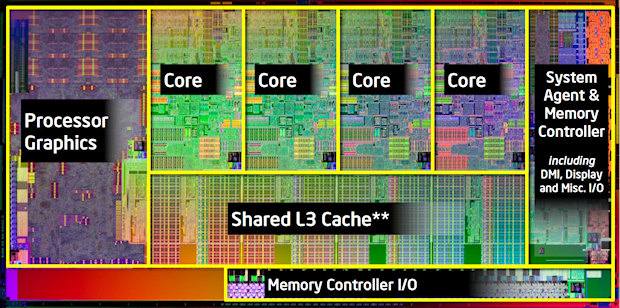
\includegraphics[scale=0.5]{sandy}
  \end{center}
  \caption{
    The figure depicts a quad-core Sandy Bridge microprocessor (or chip). The
    author was unable to locate an image of an octa-core chip.
  }
  \label{fig:p5}
\end{figure}

\subsection{Interconnecting chips to form larger SMPs}

Multiple Sandy Bridge chips can be connected to form larger modules in SMP
configurations. On Vilje, two chips are run in SMP mode on each compute node.
Thus, up to 16 (32) processors share memory.

\subsection{Interconnecting nodes to form a distributed SMP}

Multiple nodes may also be connected to form clusters or distributed SMPs. In
this case, data from one node to another must be passed across a high bandwidth
low-latency switch network. A system based on multiple nodes must therefore be
treated as a distributed memory system (at least globally).

\subsection{Key data for Vilje}

Vilje is based on 1404 nodes. The total number of processors (or cores) is
therefore 22464.

Each node represents a shared memory system with 2 octa-core Sandy Bridge chips
which share 32 GB memory (although a few nodes have 128 GB memory).

Each i7 processor operates at a clock rate of 2.6 GHz. The size of the L1 cache
(3 clocks) is 32 kbyte for data and 32 kbyte for instructions. The size of the
L2 cache (8 clocks) is 256 kbyte, while the size of the shared off-chip L3 cache
is 20 Mbyte.

\section{Programming models}

We have seen that a node (with 16 physical processors) on Vilje represents a
shared memory system where the aggregate memory for the node is globally
available to all the 16 processors. A shared memory programming model (i.e.
OpenMP) can therefore be used within a single node.

If we want to develop programs which can run on more than one node, we need to
use message-passing (i.e. MPI). This is also the programming model we will
emphasize in this course. Even though each node represents a shared memory
system, the message-passing programming model may still be used within a node.
However, the opposite is not true: a shared programming model cannot be used on
a ``pure'' distributed memory system (e.g. on a PC cluster).

Note that a system like Vilje, which represents a shared memory system within a
node, and a distributed memory system across the nodes, can also be programmed
using both programming models within a single program.

\section{Message passing}

Message passing is fundamentally processor-to-processor communication. Only a
local, unique memory is directly available to each processor. Both local and
remote processes must cooperate in order to exchange data and/or synchronize (at
least originally---some changes have been made in the extended version MPI-2).

Note that message-passing is a good way to use distributed shared memory
machines (ccNUMA) because it provides a way to express memory/data locality.

Some of the key advantages of the message-passing model are:
\begin{itemize}
\item {\em Portability}: the model can be used on a collection of
homogeneous or heterogeneous processors connected by a fast or a slow
communication network;
\item {\em Performance}: the approach exploits data locality, as well as the
availability of a large, aggregate memory;
\item {\em Expressiveness}: a limited communcation library suffices for most applications.
\end{itemize}

The Message Passing Interface (MPI) is the de facto standard for message
passing. It is a \emph{library}, not a language. MPI provides efficiency,
portability and functionality. It represents a standardized communcation library
running on a vast number of machines and architectures.
\autoref{fig:message_passing_model} illustrates the message passing model.

The original (1994) MPI-library represents the message passing model where both
the local and remote processes cooperate e.g. via a send and receive
operation. MPI-2 represents an extension of MPI where features like one-sided
messages, parallel I/O, etc. are included.

\begin{figure}
  \centering
  \begin{tikzpicture}[
    proc/.style={shape=circle, draw=darkblue, fill=cadet, thick},
    msg/.style={shape=rectangle, draw=darkblue, fill=cadet, thick, rounded corners=0.5mm},
    env/.style={minimum height=1.7cm, minimum width=1.7cm},
    scale=0.7,
    ]
    \node[proc] (p0) at (0,0) {$P_0$};
    \node[proc] (p1) at (1,3) {$P_1$};
    \node[proc] (p2) at (3,-0.6) {$P_2$};
    \node[proc] (p3) at (6,3.6) {$P_3$};
    \node[msg] (msg) at (4.0, 1.5) {\scriptsize Message};
    \node[msg, env, fill=cadet!55] (env) at (8, -2.0) {};
    \node[msg, very thin] (body) at (8, -1.7) {\scriptsize Body};
    \node[below of=body, node distance=6mm] {\scriptsize Envelope};
    \draw[->, thick] (p2) edge[bend right] node [right] {} (msg);
    \draw[->, thick] (msg) edge[bend right] node [right] {} (p1);
    \draw[->, thick] (env) edge[bend right] node [right] {} (msg);

    \node[msg] (smp) at (-2,-2) {\scriptsize SMP};
    \draw[->, thick] (smp) edge[bend left] node [right] {} (p0);
  \end{tikzpicture}
  \caption{
    The message passing model. A number of processes, $P_0, P_1, \ldots,
    P_{n-1}$, are coupled together via a fast or a slow communication network.
    Each process has a local and unique memory/cache, and each process is
    associated with a particular computational task. The individual processes
    must communicate via explicit message passing. A message consists of an
    ``envelope'' which contains sufficient information about whether and when to
    open the message, as well as information regarding how to interpret the
    ``body'' of the message (the actual data). Note that the message is the only
    means of exchanging data between the processes and/or syncronizing the
    processes.
  }
  \label{fig:message_passing_model}
\end{figure}

The MPI operations can be classified in a few types of operations:
\begin{itemize}
\item one-to-one;
\item one-to-all;
\item all-to-one;
\item all-to-all.
\end{itemize}
The first type is also referred to as point-to-point operations (send and
receive), while the last three types are collective operations.

When we here talk about ``all'', we generally mean all processes $P_0, P_1,
\ldots, P_{n-1}$ within a group of $n$ processes. Such a group defines a
\emph{communicator} and the particular process number is referred to as the
\emph{rank} within that communicator. The default is to let all processes be
members of the same (default) communicator. However, it is also possible to have
some of the processes be members of one communicator (or group), while others be
members of a different communicator. In this context, ``all'' means all the
processes \emph{within} a particular communicator.

Finally, the collective operations can be further broken down into the
following categories:
\begin{itemize}
\item data movement (broadcast; gather/scatter);
\item collective computation (max/min; sum; etc.).
\end{itemize}

We will later explain in more detail the various MPI operations. A good way to
learn MPI is by implementing a few simple examples. The whole library contains
about 125 functions. However, as few as 6 may suffice for some problems. You
only need to learn the functions needed for your particular problem. You may not
have to learn the details of the whole library even for advanced applications.

\subsection{An example}

We now discuss a brief example of a program where the MPI library is used. The
program listed below does the following: processor 0 sends a text message
``Hello, world'' to all the other processors. The other processors receive the
message and all processors print out the message together with the their own
process number.

Listings \ref{lst:mpi-hello-c} and \ref{lst:mpi-hello-fortran} show how this is
done in both C and Fortran.

\begin{lstlisting}[style=c, float, caption={Hello world MPI in C.}, label=lst:mpi-hello-c]
  #include <stdio.h>
  #include "mpi.h"

  int main(int argc, char **argv)
  {
    int rank, size, tag, i;
    MPI_Status status;
    char message[20];

    MPI_Init(&argc, &argv);
    MPI_Comm_size(MPI_COMM_WORLD, &size);
    MPI_Comm_rank(MPI_COMM_WORLD, &rank);

    tag = 100;

    if (rank == 0) {
      strcpy(message, "Hello, world");
      for (i = 1; i < size; i++) {
        MPI_Send(message, 13, MPI_CHAR, i,
                 tag, MPI_COMM_WORLD);
      }
    }
    else {
      MPI_Recv(message, 13, MPI_CHAR, 0,
               tag, MPI_COMM_WORLD, &status);
    }

    printf("node %d: %13s\n", rank, message);

    MPI_Finalize();

    return 0;
  }
\end{lstlisting}

\begin{lstlisting}[style=fortran, float, caption={Hello world MPI in Fortran.}, label=lst:mpi-hello-fortran]
  program hello
  include 'mpif.h'

  integer rank, size, ierror, tag, status(MPI_STATUS_SIZE)
  character(12) message

  call MPI_INIT(ierror);
  call MPI_COMM_SIZE(MPI_COMM_WORLD, size, ierror);
  call MPI_COMM_RANK(MPI_COMM_WORLD, rank, ierror);

  tag = 100;

  if (rank .eq. 0) then
    message = 'Hello, world'
    do i=1,size-1
      call MPI_SEND(message, 12, MPI_CHARACTER, i, tag,
                    MPI_COMM_WORLD, ierror)
    enddo
  else
    call MPI_RECV(message, 12 MPI_CHARACTER, 0, tag
                  MPI_COMM_WORLD, status, ierror)
  endif

  print*, 'node', rank, ':', message

  call MPI_Finalize(ierror)
  end
\end{lstlisting}

The output of the C version on the SGI Origin using $P=4$ and $P=8$ processors
is shown in Listings \ref{lst:mpi-hello-4} and \ref{lst:mpi-hello-8}.

\begin{lstlisting}[float, caption={Hello world MPI in C: $4$ processors.}, label=lst:mpi-hello-4]
  node 1: Hello, world
  node 3: Hello, world
  node 2: Hello, world
\end{lstlisting}

\begin{lstlisting}[float, caption={Hello world MPI in C: $8$ processors.}, label=lst:mpi-hello-8]
  node 5: Hello, world
  node 1: Hello, world
  node 7: Hello, world
  node 2: Hello, world
  node 3: Hello, world
  node 6: Hello, world
  node 4: Hello, world
\end{lstlisting}

Let us now comment on some of the statements here. We start with
\begin{lstlisting}[style=c]
  #include <stdio.h>
  #include "mpi.h"
\end{lstlisting}
The first statement is just a standard statement about including the header file
associated with string (character) operations and I/O. The second statement is
required if we want to use the MPI library in our program. In C, we need the
statement
\begin{lstlisting}[style=c]
  #include "mpi.h"
\end{lstlisting}
The equivalent statement in Fortran is
\begin{lstlisting}[style=fortran]
  include 'mpi.f'
\end{lstlisting}
The MPI header file provides basic MPI definitions and MPI data types.

The first MPI statement needs to be:
\begin{lstlisting}[style=c]
  MPI_Init(&argc, &argv);
\end{lstlisting}
This statement should only be called once. The last MPI statement is always
\begin{lstlisting}[style=c]
  MPI_Finalize();
\end{lstlisting}
This statement does not have to be the very last statement in your program, but
it needs to be the last MPI statement. It statement ensures a clean exit.

Note that the command line arguments are passed to the C version of
\texttt{MPI\_Init}. The corresponding Fortran version reads:
\begin{lstlisting}[style=fortran]
  call MPI_INIT(ierror);
\end{lstlisting}
Similar to a standard subroutine call in Fortran, a call to an MPI operation
also starts with \texttt{call}. The parameter \texttt{ierror} is an integer and
will return an error code in case something goes wrong. The C version also
returns an error code. Instead of the statement used in the program listed
above, we could alternatively have written
\begin{lstlisting}[style=c]
  errorcode = MPI_Init(&argc, &argv);
\end{lstlisting}
In this case, the variable \texttt{errorcode} (an integer) will contain an error
code if something goes wrong.

In general, any MPI statement in C has the format
\begin{lstlisting}[style=c]
  errorcode = MPI_Xxxxx(parameters...);
\end{lstlisting}
or simply
\begin{lstlisting}[style=c]
  MPI_Xxxxx(parameters...);
\end{lstlisting}
The particular MPI operation is given by ``Xxxxx'' where the name of the operation
always starts with a capital letter and the remaining letters are lower-case.
The number and type of parameters vary from operation to operation. For example,
\texttt{MPI\_Finalize} does not have any parameters at all.

In Fortran, any MPI statement has the format.
\begin{lstlisting}[style=c]
  call MPI_XXXXX(parameters..., ierror)
\end{lstlisting}
where the parameter \emph{ierror} returns an error code. Note that the name of
the particular MPI operation is always in capital letters.

The next two statements after the initialization of MPI are:
\begin{lstlisting}[style=c]
  MPI_Comm_size (MPI_COMM_WORLD, &size);
  MPI_Comm_rank (MPI_COMM_WORLD, &rank);
\end{lstlisting}
The first of these statements returns the total number of MPI processes, while
the second one returns the individual process number (the ``rank''). More
precisely, the process number is stored in the location pointed to by the second
argument. \texttt{MPI\_COMM\_WORLD} is the default name of the communicator (the
``univertse'') and which include all the processes. This can be changed in order
to create several separate ``universes.''

Note that the program listed in this example runs separately and independently
on every processor on a multiprocessor. We also refer to this as SPMD -
\emph{Single Program Multiple Data}. All the problems we will study in this
course will be of this type: the program running on each processor will be the
same for all the processors. However, the data each processor will operate on
will typically be different. The synchronization of the program will be implicit
via the MPI operations. We will return to this issue later.

When this program runs on a particular processor, the program does not
automatically know how many other processors are involved; this issue is taken
care of by the MPI operation \texttt{MPI\_Comm\_size}. In the multiprocess
context, the program running on an individual processor does not automatically
know what its associated process number is (who am I?); this issue is taken care
of by the MPI operation \texttt{MPI\_Comm\_rank}.

Let us now proceed to the statements
\begin{lstlisting}[style=c]
  if (rank == 0) {
    strcpy (message, "Hello, world");
\end{lstlisting}
The if-statement will only be true for one of the processes, namely, the process
with process number 0. This is also referred to as the ``root'' process. On the
root process, the string ``Hello, world'' is copied into the string variable
\texttt{message}.

For all the other processes, the if-statement will not be true, and the program
execution will move on to the MPI statement \texttt{MPI\_Recv}. This means that
all of the other processes will be waiting for the root process to send them
data. The root process sends data to the other processes in the loop
\begin{lstlisting}[style=c]
  for (i=1; i < size; i++) {
    MPI_Send(message, 13, MPI_CHAR, i,
             tag, MPI_COMM_WORLD);
  }
\end{lstlisting}
Several comments are in order here. First, note that the root process sends out
the same message (string) to all the other processes. This is done in a loop.
However, note that this loop corresponds to a \emph{sequential} execution
meaning that a message will be sent to process $1$ before process $2$ etc.

Let us now discuss the particular format in the parameter list for the operation
\texttt{MPI\_Send}. The general format for this operation is
\begin{lstlisting}[style=c]
  MPI_Send(start, count, datatype, dest, tag, comm);
\end{lstlisting}
The first three parameters (start, count, datatype) represent \emph{the data},
while the last three parameters (dest, tag, comm) represent \emph{the envelope};
see \autoref{fig:message_passing_model}.

We now explain all these parameters in some more detail.
\begin{itemize}
\item \emph{start}: initial address of the send buffer
\item \emph{count}: number of elements sent (of type \texttt{datatype})
\item \emph{datatype}: e.g. \texttt{MPI\_INT}, \texttt{MPI\_FLOAT}, \texttt{MPI\_CHAR} etc.
\item \emph{dest}: destination process (integer)
\item \emph{tag}: integer message identifier (e.g., \texttt{MPI\_ANY\_TAG})
\item \emph{comm}: an ordered group of communication processes (same for send
  and receive)
\end{itemize}

Only the root process sends a message. All the other processes are waiting to
receive a message. This is expressed by the MPI operation \texttt{MPI\_Recv}.
The general format for this operation is
\begin{lstlisting}[style=c]
  MPI_Recv(start, count, datatype, source, tag, comm, &status);
\end{lstlisting}
The first three parameters (start, count, datatype) represent \emph{the data},
while the last three parameters (dest, tag, comm, status) represent \emph{the
envelope}; again, see \autoref{fig:message_passing_model}.

Most of the parameters are similar to the MPI\_Send operation:
\begin{itemize}
\item \emph{start}: initial address of the receive buffer
\item \emph{count}: number of elements sent (of type \emph{datatype})
\item \emph{datatype}: e.g. \texttt{MPI\_INT}, \texttt{MPI\_FLOAT}, \texttt{MPI\_CHAR} etc.
\item \emph{source}: source process (integer), i.e., the process sending the message
\item \emph{tag}: integer message identifier (e.g., \texttt{MPI\_ANY\_TAG})
\item \emph{comm}: an ordered group of communication processes (same for send and receive)
\item \emph{status}: a structure providing information on the completed communication
\end{itemize}

Note that in the small example program, an explicit source is given, namely, the
root process. Alternatively, we could have used \texttt{MPI\_ANY\_SOURCE} since
each process in receive mode only expects one message. Similarly, we note that
the ``tag'' is explicitly given. Alternatively, we could have used
\texttt{MPI\_ANY\_TAG} since this parameter is not critical in our case.

One additional comment regarding the send and receive statements. This is an
example of point-to-point communication. There exists several versions of send
and receive. The type used here is called \emph{blocking} send and receive. This
means that the program running on the root processor cannot proceed until each
message has been safely sent and the send buffer can be safely used again.
Similarly, the program running on each of the other processors cannot proceed
until the expected message has been received in the receive buffer.

Let us now comment on the parameter \emph{count} used in the send and receive
statements. In the C version, the count parameter is set equal to 13, while it
is 12 in the Fortran version. The reason for this is that the \texttt{strcpy}
function in C will append \texttt{\textbackslash 0} (the null character) at the
end of the message. This is a symbol which indicates the end of the string. Even
though ``Hello, world'' comprises 12 letters (one byte per letter), the message
buffer in C requires 13 bytes of memory.

The parameter ``datatype'' in the send and receive operations has to be the same.
In this case, the type is \texttt{MPI\_CHAR} (in Fortran the corresponding data
type is called \texttt{MPI\_CHARACTER}). This is one of several predefined data
types. Other important ones include \texttt{MPI\_DOUBLE} and \texttt{MPI\_INT}.

Finally, note that the output from the programs is not in a sequential order.
The order may also change if we run the program over again.

\lstset{inputpath=code/openmp/}

\chapter{Shared memory machines}

\section{Introduction}

Thus far in the course we have considered programming parallel machines using a
distributed memory model, where several processes communicate through message
passing, using the MPI library. This has been the traditional programming model
used in the HPC community since distributed memory machines became popular
during the late eighties. One of the main benefits of this programming model is
that it can be used on all hardware, even machines that actually have a shared
memory architecture. However, it has one major drawback; parallelizing a code
typically requires substantial changes to the serial version.

In these notes we consider programming shared memory machines using a shared
memory programming model. In particular we consider parallelization using the
\emph{OpenMP} standard. In later years, technology have reached a point where
making a single processing core much faster is very challenging. In order to
keep up with Moore's law for the next decades, vendors have started integrating
several processing cores in one chip, even in processors targeted at desktop
computers. At the moment, dual core processors are the norm on the desktop, with
quad and hexacore processors being available in the high end market. All major
vendors have signaled that they expect 8-16 cores to be the norm within a few
years, and a few hundreds within a decade. This means that even for desktop
class programs, programmers need to start developing parallel programs to
utilize the available computing resources. The effect of this is a substantially
increased interest in developing programming tools which allows for code
parallization on shared memory archictures with little effort. While the
OpenMP standard, which originated in the late ninties, initially was
aimed at HPC applications, it has now been adapted much more broadly. The effort
to improve the standard for the desktop market has also largely benefited the
HPC community. The increased activity has resulted in two major revisions of the
standard in the last five years, making it quite extensive. The scope of this
document is not to give a thorough introduction to the whole API, but rather to
give an idea of the main principles, as well as what new challenges and benefits
programming using OpenMP offers compared to the traditional message
passing tools.

\section{The OpenMP programming model}

OpenMP is a C/Fortran language extension for programming shared memory parallel
machines. It is implemented and supported by most major vendors, including
Intel, AMD, IBM and Oracle (SUN). It is also available in open source compilers
such as GCC or Clang, as well as in professional versions of Microsoft Visual
Studio.

\begin{figure}
  \begin{center}
    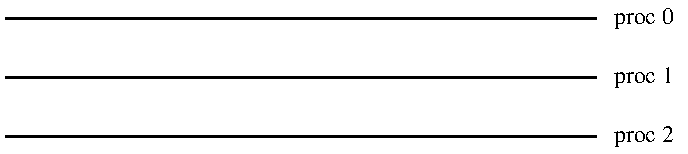
\includegraphics[width=10cm]{mpi}
  \end{center}
  \caption{
    An illustration of the MPI programming model. We have several independent
    processes, and each of these processes have their own separate program
    flow.
  }
  \label{fig:mpi}
\end{figure}

It is built on the threading paradigm in combination with a parallel section
view of the code. This means that the main program flow happens on one processor
only, which is quite a difference from the MPI programming model. Consider
\autoref{fig:mpi}, which is an illustration of the MPI programming model. Here
we have several processes, and each of these processes have their own separate
program flow. That is, each process is a separate instance of the program.
Syncronization of these processes is typically handled implicitly by using
blocking communication calls, i.e. if you call \texttt{MPI\_Send} in one
process, this process halts until it receives a confirmation that the message
has been processed. Likewise, on the receiver end, the process blocks the
program flow in the \texttt{MPI\_Recv} call until it has received the expected
message.

\begin{figure}
  \begin{center}
    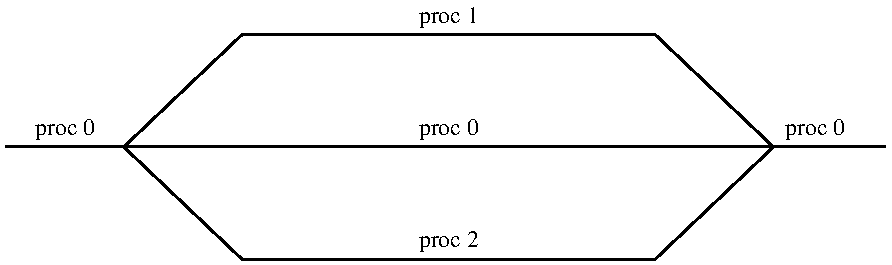
\includegraphics[width=10cm]{openmp}
  \end{center}
  \caption{
    An illustration of the \texttt{OpenMP} programming model. We only have a
    single process, hence the main program flow only happens on a single
    processor. In sections of the code that we have marked as parallel, the
    program forks into multiple threads which work independently. At the end of
    the parallel section, these threads join together again and the program flow
    is returned to the first processor.
  }
  \label{fig:openmp}
\end{figure}

In the OpenMP programming model, this is different. Consider
\autoref{fig:openmp} which is an illustration of this programming model. OpenMP
is based on a fork/join programming model, where we only have a single instance
of the program, i.e. the main program flow only happens on one processor. We
mark certain sections of the program as being suitable for parallelization. When
the program flow enters these sections of the code, the program \emph{forks}
into several threads which work independently of each other. At the end of the
code sections the threads \emph{join} with the thread running on processor 0 and
the program flow is returned to this single processor. Thus in some sense one
might say that the MPI programming model is embedded in the OpenMP model, but
only in those parts of the code we have marked as parallel sections. This is
only half the truth though. In MPI each process have their own \emph{private}
resources. Here however, this is not true. The threads within the parallel
sections all have access to the \emph{same} resources. This is crucial to keep
in mind when designating the parallel sections of the code. One of the more
common pitfalls is several threads trying to write to the same memory location,
often due to using shared buffers during the calculations. It is thus highly
recommended that you try to design your parallel sections in such a way that
each thread has its own separate working buffers.

\subsection{Critical section}
\label{sec:critsec}

If for some reason you cannot avoid several threads needing write access to the
same resources, your only choice is to construct a critical section in your code
to protect these resources. Consider \autoref{fig:cs}. A critical section of the
code is a section of the program in which only a single thread can be at any
point in time. We construct such sections of the code using a tool known as a
\emph{mutual exclusion lock}, commonly referred to as a \emph{mutex}. We make a
section of the code critical by embedding it in a lock/unlock procedure. Prior
to entering the critical section of the code, the thread requests a lock of the
mutex. If the mutex is open when this is requested, the mutex is locked, and
info about which thread has the key is recorded. This mutex is now locked until
the thread associated with the key requests an unlock. The thread then moves on
executing the critical section of the code. Upon completion of the critical
section the thread unlocks the mutex and continues doing whatever we have told
it to do next. Now, if a second thread attempts to lock the mutex while it still
is locked, the second thread will stall in the lock call until it is able to
obtain the key. Since the mutex only has a single key, it would only be able to
obtain this key after the mutex has been unlocked by the thread which is
currently holding it. Since this unlocking only happens after the critical
section has been executed, we can then guarantee that only a single thread is
within the critical section of the code at any time. We stress that this is
something you should only use if there is no way around it, since the use of a
mutex leads to a \emph{serialization} of the critical section code. This can be
catastrophic for the parallel performance of your code if a large part of the
computation time is spent within such critical sections. Since this is meant to
be a brief introduction, we will not discuss these issues further in the
following.

\begin{figure}
  \begin{center}
    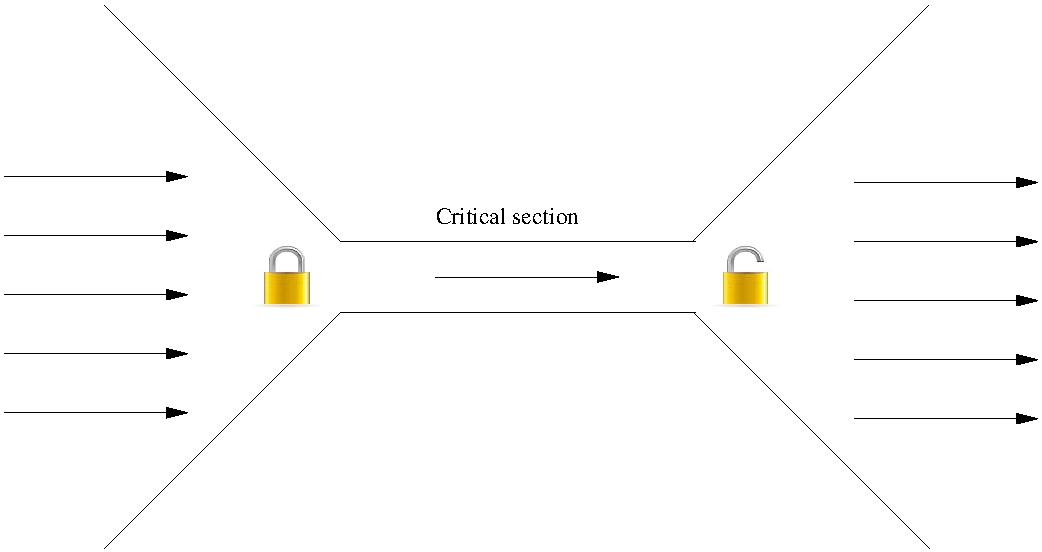
\includegraphics[width=10cm]{CriticalSection}
  \end{center}
  \caption{
    Illustration of a critical section. The incoming arrows represents the
    threads. All the threads are running concurrently, until they need to enter
    the critical section. Since only one thread can be inside the critical
    section at any time, the threads which want to enter need to wait until they
    obtain the key to the mutual exclusion lock, and hence their turn to enter
    the code section.
  }
  \label{fig:cs}
\end{figure}

\section{How to use OpenMP}

The idea behind the OpenMP API is that we give the compiler instructions on
which sections of the code we want to be parallelized. This means that, in
contrast to MPI, which works with all compilers, OpenMP requires specific
support in the compiler. The compiler then handles work division between the
available number of threads. This is in stark contrast to MPI where work
division is something the programmer always have to decide up front, before
modifying the serial code accordingly.

These instructions to the compiler are known as \emph{pragma} commands. There
are mainly two classes of OpenMP pragmas. The first class of pragmas are those
which can be used in combination with loop constructs such as \emph{for} loops.
This is the most useful case in context of HPC, since the programs typically
consist of multiple loops which apply the same operation to large datasets.
Consider the serial snippet
\lstinputlisting[style=c]{serial-for.c}
or the equivalent in Fortran
\lstinputlisting[style=fortran]{serial-for.f}

For simplicity, we here assume that \texttt{DoSomething(i)} does not depend on
any global resources, such as temporary working buffers. Hence this loop is
highly suitable for parallelization using OpenMP. In addition we first assume
that \texttt{DoSomething(i)} has a constant cost. To divide this loop among
several threads, we simply do
\lstinputlisting[style=c]{openmp-for.c}
Here we have our first example of an OpenMP directive. The pragma can be broken
down into three parts.
\begin{description}
\item[\texttt{\#pragma omp}] all \texttt{OpenMP} directives start with this.
\item[\texttt{parallel for}] instructs the compiler that we want the following
  \texttt{for}-construct parallelized.
\item[\texttt{schedule(static)}] instructs the compiler to hand each thread
  approximately the same number of loop iterations up front. This is a good
  solution here since (we have assumed that) each call to
  \texttt{DoSomething(i)} has the same cost. Hence such a simple division will
  give good load balancing between the threads.
\end{description}
The ingredients in the Fortran version is the same, but the syntax is slightly
different.
\lstinputlisting[style=fortran]{openmp-for.f}
To avoid having to restate everything twice, we only give C examples in the
following.

We can also run into situations where each call to \texttt{DoSomething(i)} has a
different cost. One example where you can run into this scenario is if
\texttt{DoSomething(i)} consists of an iterative method such as conjugate
gradients. Each solution process can have a different solution time. In this
case, if we give each thread a fixed number of loop iterations up front, we end
up with poor load balancing between the threads. Fortunately OpenMP offers a
mechanism to handle these situations. We simply do
\lstinputlisting[style=c]{openmp-for-dynamic.c}
The only difference is the change of the schedule parameter in the pragma from
static to dynamic. We here instruct the compiler to use a dynamic workload
division between the threads. This means that we reserve one thread as a
bookkeeper/negotiator. Within this parallel section this thread has a simple
task; keep track of which loop iterations have been performed and hand out a new
one to a thread when it requests it. Initially each thread is given a single
loop iteration to perform. Once the thread finishes this, it asks the negotiator
thread for a new one. The threads keep doing this until all work has been
performed.

If \texttt{DoSomething(i)} is fairly costly, this works very well. However, in
some cases each DoSomething(i) may be rather cheap. In this case the cost of
asking the negotiator for a new loop iteration between every calculation may
dominate the actual computation time. OpenMP also offers a mechanism to try to
minimize this problem. Instead of having the negotiator hand out a single loop
iteration when a thread asks for more work, it can hand out loop iterations in
chunks. Consider
\lstinputlisting[style=c]{openmp-for-dynamic-chunk.c}
The second parameter in the schedule (5) is the \emph{chunk size}. This is the
number of loop iterations a thread is (at most) given when it requests more work
from the negotiator thread. Thus we can limit the number of times a thread has
to communicate with the negotiator, hopefully making this part of the process
less dominating.

OpenMP also offers a third scheduling mode, called \emph{guided}. Consider
\lstinputlisting[style=c]{openmp-for-guided-chunk.c}
This is essentially a variant of dynamic scheduling, where we start out with a
large chunk size. The chunks are then exponentially decreased until we reach a
minimum, as specified in the chunk size. The idea here is that allocating large
chunks initially is good for performance, since these will typically overlap
fairly well. However, when the number of loop iterations left is small, we may
end up in a situation where all the remaining loop iterations are allocated to a
single thread. This is bad for performance since the other threads would then be
left idle. By using progressively smaller chunks, the chance of this happening
is reduced.

The second class of OpenMP directives are not tied to loop constructs. Instead
they are to be used if we have sections of the code which are completely
independent of each other. Consider the snippet
\lstinputlisting[style=c]{serial-sections.c}
If we are certain that these jobs are independent of each other, we can tell the
compiler this fact, and ask for the different \emph{sections} to be executed in
parallel on several threads. We do
\lstinputlisting[style=c]{openmp-sections.c}
Here each section of the code would be performed in a separate thread, before
the program flow again returns to processor 0 once all sections have been
completed. This directive is not as useful as those used in combination with
loop constructs, in particular we cannot as easily utilize a large number of
threads. The reason for this is fairly straight forward. In this example we can
at most use three threads, since there are only three sections of code
specified. It is often hard to find a large number of independent code sections
to allow for a larger number of threads. Large, expensive loops, however, are
typically present in most codes.

\section{$\pi$ --- OpenMP style}
We have previously calculated $\pi$ in both serial and MPI codes. We can
certainly use OpenMP for this as well. In the original serial code we have a
loop
\lstinputlisting[style=c]{serial-integrate.c}
This is the loop where the main work happens, and is what we should focus our
effort on. In this case, it is embarassingly simple to parallelize the loop
since there are no dependencies between the loop iterations. We can simply hand
a number of iterations to each thread, and then sum up the results afterwards.
OpenMP makes this convenient through the reduction directive
\lstinputlisting[style=c]{openmp-integrate.c}

\section{Compiling and running an \texttt{OpenMP} application}

We have a source file called \emph{openmp.c}, and we want to compile this with
OpenMP directives enabled. On a standard Linux computer this can be achieved by
using the \texttt{-fopenmp} directive, i.e.
\begin{lstlisting}
  gcc -O3 -o openmp -fopenmp -c openmp.c
\end{lstlisting}
while using the Intel compiler as we do on Kongull or Vilje, the directive is
simply \texttt{-openmp}, i.e.
\begin{lstlisting}
  icc -O3 -o poisson -openmp -c poisson.c
\end{lstlisting}
As long as we do not use any OpenMP utility function calls, we can still compile
this code into a completely serial code, simply by removing the compiler
switches. The compiler then simply ignore the pragmas, which makes the code look
exactly as the serial code from its point of view. This is in stark contrast to
a MPI version of the code where we would have to do substantial changes which
makes the program dependent on the MPI libraries.

To run our program using for instance four threads we do
\begin{lstlisting}[style=c]
  OMP_NUM_THREADS=4 ./openmp 2048
\end{lstlisting}

\section{Final remarks}

Modern supercomputers typically consist of multiple SMP nodes interconnected in
a NUMA organization, see the lecture notes. Clusters also fall into the same
category, since even the commodity processors used here have several cores
integrated in their chips as discussed in the introduction. In particular, Vilje
is an example of such a machine. Here each SMP node consists of 16
hyper-threaded processor cores. This means that an application which is
parallelized using OpenMP can at most use 32 threads, although for floating
point dominated programs, running only one thread per physical core is adviced.
If more computing resources is needed, we have no choice but to resort to a
distributed memory approach using MPI. The same applies to Kongull, except here
each SMP has 12 cores, which are not hyperthreaded.

A very natural question to ask is whether or not the two approaches can be
combined. The answer to this is yes. In fact this approach often allows us the
best of both worlds. Fine-grain parallelism is often intricate to exploit using
a distributed memory model, while the convenience offered by the shared memory
model often makes it fairly trivial to express. In addition, it is not always
easy to say up front where exploiting fine-grained parallelism actually will
improve the performance of your program. Since the modifications to the program
using the OpenMP approach is minimal, we do not have to invest much effort just
to benchmark whether or not parallizing a particular loop improves performance.

Coarse-grain parallelism, however, is often fairly involved to exploit using a
shared memory model, in particular due to the complications involved in
protecting shared resources such as working buffers. This often lead to
excessive memory usage or serialization of substantial parts of the code through
usage of critical sections, see \autoref{sec:critsec}. Using a distributed
memory model, this problem is nonexistent. Each process have their own private
resources which are inaccessible from the other processes. Here expressing
coarse grain parallelism is often just a matter of adjusting the limits on some
loops, as well as adding the appropriate library calls for data exchanges
between the processes when such exchanges are needed.

Hence a program where we utilize a message passing based approach, i.e. MPI, to
express the coarse grain parallelism, while utilizing OpenP pragmas to express
the fine grain parallelism within each MPI process allows use to use each
approach for what they are best at, while avoiding their weak sides.

\section{Further reading}

You can find the official OpenMP homepage at \url{http://openmp.org}. This page
is a great resource for those who are interested in more details. In addition to
having the description of the standard, it also contains links to several books
on subject, as well as discussion forums where you can ask questions. If a
source of tutorials are to be suggested, we can recommend
\url{https://computing.llnl.gov/tutorials/openMP/}.

\textbf{Acknowledgements:} Stephan Diederich helped with proof reading and gave
some valuable input while this chapter was written. The chapter is written by
Arne Morten Kvarving. Your assistance was greatly appreciated.

\chapter{Basic linear algebra performance}

\section{Introduction}

Simulation-based science and technology require a rich set of numerical
algorithms. For example, in the context of numerical solution of partial
differential equations we have seen the need to solve linear systems of
algebraic equations. Solution algorithms for linear system of equations may
again be classified as direct methods or iterative methods. In either case, the
solution algorithms rely on basic linear algebra operations. Most of the
floating point operations in a typical simulation code are associated with such
operations.

Because of the importance of basis linear algebra operations, a special library
called BLAS (\emph{Basic Linear Algebra Subroutines}) has been developed to deal
with such operations. The BLAS library is again classified into three levels:
\begin{itemize}
\item Level 1 operations: vector-vector operations;
\item Level 2 operations: matrix-vector operations;
\item Level 3 operations: matrix-matrix operations.
\end{itemize}
Two examples of level 1 BLAS operations are
\begin{align}
  \bm y := a \bm x + \bm y
  \label{eq:daxpy}
\end{align}
and
\begin{align}
  \sigma = \bm x \cdot \bm y = \bm x^\intercal \bm y
  \label{eq:dot}
\end{align}
Operation \eqref{eq:daxpy} is called a {\em daxpy} operation. Here, the input
$\bm x$ of length $n$ is scaled with a constant $a$ and added to the second
input vector $\bm y$, which is also of length $n$. The result is then stored
back in the vector $\bm y$, i.e. the original values in $\bm y$ are overwritten.

Operation \eqref{eq:dot} represents a dot product (or inner product) which we
have discussed extensively earlier in the course. Here, from the two input
vectors $\bm x$ and $\bm y$ (both of length $n$) we compute the scalar $\sigma$.

An example of a level 2 BLAS operation is the matrix-vector product
\begin{align}
  \bm y = \bm A \bm x
  \label{eq:mvp}
\end{align}
Here, the output vector $\bm y$ (of length $m$) is computed from the given input
matrix $\bm A$ (of dimension $m \times n$) and the given input vector $\bm x$
(of length $n$).

An example of a level 3 BLAS operation is the matrix-matrix product
\begin{align}
  \bm C = \bm A \bm B
  \label{eq:mxm}
\end{align}
Here, the matrix $\bm X$ (of dimension $m\times n$) is computed as the product
of the matrix $\bm A$ (of dimension $m\times k$) and the matrix $\bm B$ (of
dimension $k\times n$).

In this set of lecture notes, we will discuss the performance of operations
\ref{eq:daxpy}, \ref{eq:dot} and \ref{eq:mxm} on Vilje. We will primarily focus
on the single-processor performance, but we will also consider the
multi-processor performance using the BLAS implementation included in the MKL
library developed at Intel.

In particular, we will discuss the performance as a function of:
\begin{itemize}
\item basic linear algebra operation;
\item programming aspects;
\item high level programming languages;
\item exploiting multiple threads.
\end{itemize}

\subsection{Key data for Vilje}

The current supercomputer at NTNU, Vilje, is based on 1404 nodes. The total
number of processors (or cores) is 22464 physical cores, each core being
hyperthreaded, thus having 44928 logical cores.

Each node represents a shared memory system with 2 octave-core Sandy Bridge
chips which share 32 GB memory (although a few nodes have 128 GB memory).

Each processor operates at a clock rate of 2.6 GHz. The size of the private L1
cache is 32 kbyte for data and 32 kbyte for instructions. The size of the
private L2 cache is 256 kB, while the size of the off-chip L3 cache is 20 Mbyte.

The latency associated with the different memory levels is: 8 clock cycles for
L2, 30 clock cycles for L3, and 150 clock cycles for main memory.

\subsection{Maximum theoretical performance}

The maximum theoretical performance (or peak performance) is the maximum number
of floating point operations completed per second. We may talk about the maximum
theoretical performance for a single CPU, a single node, or for the entire
machine.

The maximum theoretical performance of a single core of a Sandy Bridge chip is
found as follows. First, each physical has a separate SIMD floating point unit
(AVX). This is a superscalar/FMA capable (Fused Multiply and Add) vector unit
which can operate on 4 double precision number simultaneously. This performance
is achieved if the units can be filled fast enough with data, and after a
certain start-up period (recall the earlier discussion about pipelining). With 1
AVX per physical core, the maximum theoretical performance per core is thus 8
floating point operations per clock cycle. With a clock cycle of 2.6 GHz, this
translates into 21 Gflops per physical core. Note, since logical cores share AVX
units, we cannot expect additional performance from using the hyperthreads,
since in order to achieve this performance we are already using the full memory
bandwidth of the machine.

Unfortunately, many operations only achieve a fraction of the maximum
theoretical performance. The measured performance will typically depend on the
the reuse of data (a high degree of reuse means less memory traffic) and how
good the compiler is. For the basic linear algebra operations we will study
here, we will see a large variation in performance. Not surprisingly, the
specially developed BLAS library will typically give excellent performance.
However, some of the observed differences may come as a surprise.

\section{Compiling and running the programs}

The source code and the buildsystem for the tests are found in the git
repository at \url{https://github.com/akva2/tma4280}. CMake is used to generate
the different Fortran programs, and to generate a build system capable of
building the testing suite on most machines, including Vilje, Kongull or your
local Linux/OSX machine. There is also a example job script (for Vilje, it needs
some small changes for Kongull), a script to postprocess the results and (for
those interested) the Octave/Matlab scripts used to generate the \LaTeX~code
for the tables in this document.

\section{Vector-vector operations}

In this section we briefly discuss some performance results for an important
vector-vector operation: the daxpy-operation \eqref{eq:daxpy}, which named as
such: \textbf{d}ouble precision \textbf{a}lpha $\bm x$ \textbf{p}lus $\bm y$.
\[
  \bm y := \alpha \bm x + \bm y,
\]
does exactly $n$ operations (additions) on $\mathcal{O}(n)$ data, and needs to
store $n$ floating point numbers back into memory. All this memory traffic will
severely influence the performance we can reach. In contrast to the
matrix-matrix multiplication, only $\mathcal{O}(1)$ floating point operations
are needed per floating point number stored. There is thus very little "reuse"
of data in vector-vector operations. From these general considerations we expect
vector-vector operations to perform significantly worse than the matrix-matrix
product multiplication.

\subsection{Performance results for daxpy}

\Autoref{tab:tab9, tab:tab10} show the performance results of the daxpy
operation. In general, a standard implementation of the daxpy operation in C
(i.e., a single loop), performs just fine. This is to be expected since this
operation is utterly memory bandwidth bound and not much can be done wrong.

\begin{table}
  \caption{
    Performance results (in MFlops) for a standard daxpy implementation in C
    (implemented as a single loop), compared with the performance using BLAS.
  }
  \label{tab:tab9}
  \begin{center}
  \bgroup\def\arraystretch{1.2}
  \begin{tabular}{c|rrrr|r}
    \hline
    $n$ & \texttt{-O0} & \texttt{-O1} & \texttt{-O2} & \texttt{-O3} & BLAS \\
    \hhline{======}
    $10^2$ & 45.92 & 63.69 & 82.82 & 68.37 & 0.10 \\
    $10^3$ & 227.13 & 363.00 & 457.12 & 434.61 & 0.81 \\
    $10^4$ & 403.55 & 1122.64 & 1217.60 & 1246.42 & 7.76 \\
    $10^5$ & 415.85 & 1300.58 & 1322.22 & 1338.98 & 79.71 \\
    $10^6$ & 379.52 & 418.88 & 413.65 & 413.65 & 341.52 \\
    $10^7$ & 376.78 & 420.55 & 413.65 & 420.36 & 341.52 \\
    \hline
  \end{tabular}
  \egroup
\end{center}

\end{table}

\begin{table}
  \caption{
    Performance results (in MFlops) for a standard daxpy implementation in
    Fortran (implemented as a single loop), compared with the performance using
    BLAS.
  }
  \label{tab:tab10}
  \begin{center}
  \bgroup\def\arraystretch{1.2}
  \begin{tabular}{c|rrrr|r}
    \hline
    $n$ & \texttt{-O0} & \texttt{-O1} & \texttt{-O2} & \texttt{-O3} & BLAS\\
    \hhline{======}
    $10^2$ & 0.07 & 0.07 & 0.08 & 0.07 & 0.10 \\
    $10^3$ & 0.89 & 0.83 & 0.67 & 0.69 & 0.80 \\
    $10^4$ & 9.37 & 7.23 & 8.17 & 7.30 & 7.75 \\
    $10^5$ & 70.96 & 66.18 & 70.65 & 87.33 & 79.70 \\
    $10^6$ & 353.27 & 356.28 & 385.78 & 402.52 & 341.51 \\
    $10^7$ & 513.54 & 514.07 & 514.52 & 512.66 & 341.51 \\
    \hline
  \end{tabular}
  \egroup
\end{center}

\end{table}

\section{Matrix-matrix multiplication}

Let us first consider the matrix-matrix multiplication \eqref{eq:mxm}. In
general, if $\bm A \in \mathbb{R}^{m \times k}$, $\bm B \in \mathbb{R}^{k \times
n}$ and $\bm C \in \mathbb{R}^{m \times n}$,
\[
  c_{ij} = \sum_{l=1}^k a_{il}b_{lj}, \qquad
  \forall\ i=1,\ldots,m, \qquad
  \forall\ j=1,\ldots,n.
\]
Written out, this is
\[
  c_{ij} = a_{i1}b_{1j} + a_{i2}b_{2j}+\cdots+a_{ik}b_{kj} \qquad
  \forall\ i=1,\ldots,m, \qquad
  \forall\ j=1,\ldots,n.
\]
Mathematically, there are thus $k$ multiplications and $k-1$ additions for each
index $i,j$. The total number of operations is then
\[
  \mathcal{N}_\text{op} = mn\left(2k-1\right).
\]

For the special case where $A,B,C\in \mathbb{R}^{nxn}$, the total number of operations is
\[
  \mathcal{N}_\text{op} = n^2²\left(2n-1\right) \approx 2n^3.
\]
Hence, if $m,n,k$ are of the same order (e.g., $m=k=n$),
\begin{align}
  \mathcal{N}_\text{op} = \mathcal{O}(n^3).
\end{align}

\subsection{Triple-nested loop}

In a numerical program, matrix multiplication can be implemented in several ways.
The most straightforward method is in a triple-nested loop as follows (using C).
\begin{lstlisting}[style=c]
  for(i=0; i<m; i++) {
    for(j=0; j<n; j++) {
      c[i][j] = 0.0;
      for(l=0; l<k; l++) {
        c[i][j] += a[i][l]*b[l][j];
      }
    }
  }
\end{lstlisting}
Here, the terms are accumulated relative to an initialized value of zero.
Counting the number of floating point operations in the inner-most loop, there
are one multiplication and one addition. The total number of floating point
operations for matrix multiplication then becomes $\mathcal{N}_\text{op} = 2mnk$
( $=2n^3$ when $m=k=n$).

\subsection{Loop unrolling}

Loop unrolling helps to make the data flow and the data dependencies more
explicit and prepare for good use of the floating point units. For example, when
$k=10$, the inner-most loop can be unrolled manually to get the following
alternative version:
\begin{lstlisting}[style=c]
  for (i=0; i<m; i++) {
    for (j=0; j<n; j++) {
      c[i][j] = a[i][0]*b[0][j]
              + a[i][1]*b[1][j]
              + a[i][2]*b[2][j]
              + a[i][3]*b[3][j]
              + a[i][4]*b[4][j]
              + a[i][5]*b[5][j]
              + a[i][6]*b[6][j]
              + a[i][7]*b[7][j]
              + a[i][8]*b[8][j]
              + a[i][9]*b[9][j];
    }
  }
\end{lstlisting}
Here, all the terms are written out explicitly, following the mathematical
definition. The computation of \texttt{c[i][j]} now takes one addition fewer.

Loop unrolling reveals independent operations that can be performed
concurrently, while reducing the index-related overhead of the loop. This makes
it possible to make better use of the pipelined, superscalar (vector) floating
point units of the processor. At high enough optimization levels, the compiler
will typically try to unroll loops where it sees this as beneficial.

\subsection{Performance results}

We now present performance measurements for the matrix-matrix multiplication.
The source codes used are given in the appendix. In all the tests we perform,
$m=k=n$ (i.e., we consider square matrices). Both a C version and a Fortran
version of the matrix-matrix operation will be tested and compared with the
performance using the \texttt{dgemm} routine from the BLAS library. We provide
the full program listings, together with a description of how the programs were
compiled and run on Vilje. For example, we will explore the effect of using
different levels of compiler optimization.

Note that we may call the Level 3 BLAS routine \texttt{dgemm} from either
Fortran or C. When we use this library routine, the optimization level or code
language should not matter. As long as $n$ is large enough, it is possible to
obtain a high degree of peak performance.

Finally, note that the performance results we list in the following are
approximate and may not be exactly reproducable. However, they represent typical
results and the conclusions we arrive at should be valid.

The programs were run on 16 processors even though the code contains no
communication between the processors. This gave 16 timing results per run.

These versions are single threaded; the difference is only the compiler
optimization level.

\begin{table}
  \caption{Standard mxm (triple-nested loop) using C, compared with BLAS.}
  \label{table:tab1}
  \begin{center}
  \bgroup\def\arraystretch{1.2}
  \begin{tabular}{c|rrrr|r}
    \hline
    $n$ & \texttt{-O0} & \texttt{-O1} & \texttt{-O2} & \texttt{-O3} & BLAS \\
    \hhline{======}
    100 & 274.55 & 566.00 & 562.76 & 563.32 & 775.64 \\
    500 & 226.53 & 503.96 & 496.40 & 496.84 & 14323.68 \\
    1000 & 180.78 & 214.33 & 214.37 & 214.36 & 16786.90 \\
    1500 & 169.95 & 205.26 & 204.69 & 204.55 & 17808.83 \\
    \hline
  \end{tabular}
  \egroup
\end{center}

\end{table}

As can be seen from \autoref{table:tab1}, the compiler optimization level had
really disappointing influence on the obtained performance---in fact, it
actually reduced it in some cases. These results looks far from flattering for
the C programming language. Fortunately, this can be overcome by using BLAS, in
this case through MKL. The BLAS version of the program was invoked by calling
e.g.

\begin{lstlisting}[style=shell]
  mpirun -np 16 timing-O3 1000 2
\end{lstlisting}

For the Fortran version of the programs, however, as can be seen from
\autoref{table:tab2}, the compiler optimization level greatly influences the
obtained performance.

\begin{table}
  \caption{
    Standard $m \times m$ (triple-nested loop) using Fortran, compared with
    BLAS.
  }
  \label{table:tab2}
  \begin{center}
  \bgroup\def\arraystretch{1.2}
  \begin{tabular}{c|rrrr|r}
    \hline
    $n$ & \texttt{-O0} & \texttt{-O1} & \texttt{-O2} & \texttt{-O3} & BLAS \\
    \hhline{======}
    100 & 247.37 & 1666.47 & 4800.47 & 7109.23 & 775.64 \\
    500 & 191.22 & 982.85 & 3375.70 & 7565.13 & 14323.68 \\
    1000 & 142.11 & 210.15 & 1356.46 & 7228.42 & 16786.90 \\
    1500 & 122.92 & 205.13 & 1357.79 & 7584.47 & 17808.83 \\
    \hline
  \end{tabular}
  \egroup
\end{center}

\end{table}

We see that the language utilized greatly influnces the performance of this
operation. This can be attributed to the fact that, given proper memory
handling, the matrix times matrix operation is dominated by floating point
operations. The BLAS and (and to some extent) Fortran realizations manage to
keep the pipelines filled with data, while the C version does not seem to be
able to keep the floating point units fully occupied.

Let us also compare these performance results with the manually unrolled
innermost loop (which we have done for the specific case $n=10$). The programs
are compiled and linked as before. When we activate \texttt{mxm\_unr}, we obtain
the results in \Autoref{table:convergence_C, table:convergence_F}.

\begin{table}
  \caption{``Manually'' unrolled innermost loop (\texttt{mxm\_unr}), C.}
  \label{table:convergence_C}
  \begin{center}
  \bgroup\def\arraystretch{1.2}
  \begin{tabular}{c|rrrr}
    \hline
    $n$ & \texttt{-O0} & \texttt{-O1} & \texttt{-O2} & \texttt{-O3} \\
    \hhline{=====}
    10 & 328.19 & 485.23 & 577.84 & 409.26 \\
    \hline
  \end{tabular}
  \egroup
\end{center}

\end{table}

\begin{table}
  \caption{``Manually'' unrolled innermost (\texttt{mxm\_unr}), Fortran.}
  \label{table:convergence_F}
  \begin{center}
  \bgroup\def\arraystretch{1.2}
  \begin{tabular}{c|rrrr}
    \hline
    $n$ & \texttt{-O0} & \texttt{-O1} & \texttt{-O2} & \texttt{-O3} \\
    \hhline{=====}
    10 & 189.17 & 292.61 & 674.69 & 621.29 \\
    \hline
  \end{tabular}
  \egroup
\end{center}

\end{table}

We do not observe much performance increase for either case. It seems that this is a trick
the compiler uses extensively on its own. Note that the Fortran version is still
about 50\% faster than the C version (for \texttt{-O3}).

We now try to use the parallel (multi-threaded version) of BLAS implemented in
the MKL library.
\begin{table}
  \caption{BLAS with 16 threads (SMP). All performance numbers are in MFlops.}
  \label{table:tab4}
  \begin{center}
    \bgroup\def\arraystretch{1.2}
    \begin{tabular}{cr}
      \hline
      $n$ & BLAS (16 threads) \\
      \hhline{==}
      100 & 1463.80 \\
      500 & 66599 \\
      1000 & 100527 \\
      1500 & 101389 \\
      \hline
    \end{tabular}
    \egroup
  \end{center}
\end{table}

From \autoref{table:tab4} we see that we obtain very impressive performance.
These numbers should be compared with the maximum theoretical performance for
the entire node (i.e., using 16 processors) which is $16\times 21$ GFlops $=
336$ GFlops. Note that the cannot get more than 21 GFlops per core since this
number corresponds to the maximum performance of the available multiply-and-add
units per core. We thus see that BLAS (using the SMP version of the \texttt{MKL}
library) achieves close to 33\% of the maximum theoretical performance over 16
processors. This is actually quite impressive since this was achieved only by
adding a few compile and run flags; the program itself is unchanged from
earlier. This might seem a bit disappointing, but it just shows the real
bottleneck in the computer: memory bandwidth.

Finally, we recall the reason for the excellent performance of the BLAS library
for the matrix-matrix multiplication operation: the mxm operation uses
$\mathcal{O}(n^2)$ data and $\mathcal{O}(n^3)$ operations, implying that we need
to do $\mathcal{O}(n)$ floating point operations per single floating point
number stored. Because of the significant "reuse" of data, there is a
significant potential to hide the memory latency and keep the floating point
units busy. In particular, BLAS is able to get close to optimal single-processor
performance, and a standard triple loop in Fortran is able to get fairly close
using two threads per core. Unfortunately, the C version is not able to keep the
floating point units busy enough.

\subsection{Combining Fortran and C}

We recall that memory is allocated column-wise in Fortran and row-wise in C. In
BLAS the Fortran convention is used. It is thus necessary to be careful when
using two-dimensional arrays when calint \texttt{dgemm} (or other routines
following the Fortran convention).

To ensure correctness, there are several ways to proceed. By switching indices
when accessing arrays in C, a ``pseduo'' column-wise allocation is achieved.
This is the approach we choosed to use here (and in the rest of the course).
Sometimes it may be possible to use a version of the library that accepts
row-wise allocation, such as the CBLAS library. However, CBLAS is not as
universally available, so we have chosen the approach that is most portable.

% The standard inner product (or dot product) of two vectors $x$ and $y$
% of length $n$ is given by
% \[
%         \sigma = \underline{x}^T\underline{y} = \underline{x}\cdot \underline{y} =
%         \sum_{i=1}^n x_i y_i.
% \]
% This operation requires $\mathcal{O}(n)$ floating point operations
% ($n$ multiplications and $n-1$ additions) on
% $2n = \mathcal{O}(n)$ floating point numbers, and only a
% single number ($\sigma$) needs to be stored back to memory.

% \begin{figure}
% \centering
%         \subfigure[Fortran]{\includegraphics[width=10cm]{daxpy-smp-fortran}}\\
%         \subfigure[BLAS]{\includegraphics[width=10cm]{daxpy-smp-blas}}
%         \caption{Performance of the daxpy operation in SMP mode. All programs are compiled with full compiler optimizations.}
%         \label{fig:daxpy-smp}
% \end{figure}
% \input{Table12.tex}

% \subsection{Performance results: inner product}

% Tables 7-10 show the performance of the inner product on \texttt{njord}.

% \begin{center}
  \bgroup\def\arraystretch{1.2}
  \begin{tabular}{c|rrrr|r}
    \hline
    $n$ & \texttt{-O0} & \texttt{-O1} & \texttt{-O2} & \texttt{-O3} & BLAS \\
    \hhline{======}
    $10^2$ & 45.92 & 63.69 & 82.82 & 68.37 & 0.10 \\
    $10^3$ & 227.13 & 363.00 & 457.12 & 434.61 & 0.81 \\
    $10^4$ & 403.55 & 1122.64 & 1217.60 & 1246.42 & 7.76 \\
    $10^5$ & 415.85 & 1300.58 & 1322.22 & 1338.98 & 79.71 \\
    $10^6$ & 379.52 & 418.88 & 413.65 & 413.65 & 341.52 \\
    $10^7$ & 376.78 & 420.55 & 413.65 & 420.36 & 341.52 \\
    \hline
  \end{tabular}
  \egroup
\end{center}

% \begin{center}
  \bgroup\def\arraystretch{1.2}
  \begin{tabular}{c|rrrr|r}
    \hline
    $n$ & \texttt{-O0} & \texttt{-O1} & \texttt{-O2} & \texttt{-O3} & BLAS\\
    \hhline{======}
    $10^2$ & 0.07 & 0.07 & 0.08 & 0.07 & 0.10 \\
    $10^3$ & 0.89 & 0.83 & 0.67 & 0.69 & 0.80 \\
    $10^4$ & 9.37 & 7.23 & 8.17 & 7.30 & 7.75 \\
    $10^5$ & 70.96 & 66.18 & 70.65 & 87.33 & 79.70 \\
    $10^6$ & 353.27 & 356.28 & 385.78 & 402.52 & 341.51 \\
    $10^7$ & 513.54 & 514.07 & 514.52 & 512.66 & 341.51 \\
    \hline
  \end{tabular}
  \egroup
\end{center}

% \begin{figure}
%         \includegraphics{inner}
%         \caption{Performance of the inner product operation in a single core,
%         single thread mode.
%         All programs are compiled with full compiler optimizations.
%         We now see that the specific programming language has less influence
%         on the performance compared to the matrix-matrix operation.
%         This can be attributed to the fact that a vector-vector operation
%         is latency bound and that the main aspect limiting the performance is
%         how fast the machine can feed the processor data.}
%         \label{fig:inner}
% \end{figure}

% \input{Table7.tex}
% \begin{figure}
%         \includegraphics{inner-smt}
%         \caption{Performance of the inner product operation in single core, SMT mode.
%         All programs are compiled with full compiler optimizations.
%         We now see that the specific programming language has less influence
%         on the performance compared to the matrix-matrix operation.
%         This can be attributed to the fact that a vector-vector operation
%         is latency bound and that the main aspect limiting the performance is
%         how fast the machine can feed the processor data.}
%         \label{fig:inner-smt}
% \end{figure}

% \input{Table8.tex}
% \begin{figure}
% \centering
%         \subfigure[FORTRAN]{\includegraphics[width=10cm]{inner-smp-fortran}}\\
%         \subfigure[BLAS]{\includegraphics[width=10cm]{inner-smp-blas}}
%         \caption{Performance of the inner product operation with $x \neq y$ in SMP mode. All programs are compiled with full compiler optimizations.}
%         \label{fig:inner-smp}
% \end{figure}


% \clearpage
% \subsection{Performance results: inner product (x=y)}

% Finally Tables 13-16 show the performance of an inner product
% when $x$ and $y$ is the same vector.

% \input{Table13.tex}
% \input{Table14.tex}
% \begin{figure}
%         \includegraphics{dot}
%         \caption{Performance of the inner product operation where $x = y$.
%                          All programs are compiled with full compiler optimizations.
%                          We see that this time the language utilized has less influnces
%                          on the performance of the operation. This can be attributed to the fact that this
%                          operation is latency bound and that the main thing limiting the performance is
%                          how fast the machine can feed the processor data.}
%         \label{fig:dot}
% \end{figure}
% \input{Table15.tex}
% \begin{figure}
%         \includegraphics{dot-smt}
%         \caption{Performance of the inner product operation where $x = y$ in SMT mode.
%                          All programs are compiled with full compiler optimizations.
%                          We see that this time the language utilized has less influnces
%                          on the performance of the operation. This can be attributed to the fact that this
%                          operation is latency bound and that the main thing limiting the performance is
%                          how fast the machine can feed the processor data.}
%         \label{fig:dot-smt}
% \end{figure}

% \input{Table16.tex}
% \begin{figure}
%         \subfigure[Fortran]{\includegraphics[width=6.5cm]{dot-smp-fortran}}
%         \subfigure[BLAS]{\includegraphics[width=6.5cm]{dot-smp-blas}}
%         \caption{Performance of the inner product operation where $x = y$ in SMP mode. All programs are compiled with full compiler optimizations.}
%         \label{fig:dot-smp}
% \end{figure}

% \end{document}

% \clearpage
% \section{Discussion}


% \subsection*{Memory limitations}
% In the vector-vector operation \emph{daxpy} a vector is multiplied with a scalar,
% and the result is added to another vector, overwriting the second vector. In Fortran
% language this will look like the following loop:
% \begin{lstlisting}[language=Fortran]
% real*8 a, x(n), y(n)
% do i = 1,n
%         y(i) = y(i) + a*x(i)
% enddo
% \end{lstlisting}
% Each iteration of the loop, the two elements $x(i)$ and $y(i)$ are loaded to registers,
% a multiply-add operation is performed on the data, and the result $y(i)$ is stored
% to memory. (In addition, some indexing work and a test for completion of the loop must be
% performed. The scalar constant a can be held in a register, without any need for extra
% memory operations.)

% The load/store unit can be used concurrently with the floating-point units.
% Each cycle, it can perform either a load or a store operation. At best,
% a store operatin in this example can be performed every third cycle, with two
% loads in between. Since the stored value is the result of one multiply-add operation,
% the maximum achievable performance for \emph {daxpy} is one third of peak performance.

% Figure \ref{fig:daxpy} demonstrates achievable performance of the daxpy operation on Njord.



% \subsection*{Data reuse in matrix multiplication}
% The key to higher performance than what was possible in the pervious example, is to perform
% more operations on the data that is being loaded, before storing the results.

% In matrix multiplication the amount of work is $\mathcal{O}\left(N^3\right)$, while the amount
% of data is $\mathcal{O}\left(N^2\right)$. Therefore, this problem has a potential for
% data resue. By rewriting the nested loop, the number of load and store operations
% can be reduce to the same as the nmber of multiply-add operations (or lower).

% The way this is accomplished is by performing outer loop unrolling. When this technique
% is used, a small block of values from one of the arrays is stored in registers for reuse.

% If both the outer loops are unrolled twice, the Fotran matrix multiplication
% loop would look similar to the following:
% \begin{lstlisting}
% do j = 1,n, 2
%         do l=1,k,2
%                 b00 = b(l,j)
%                 b01 = b(l,j+1)
%                 b01 = b(l+1,j)
%                 b11 = b(l+1,j+1)
%                 do i= 1,m
%                         c(i,j)   = c(i,j)   + a(i,1)  *b00
%                         c(i,j+1) = c(i,j+1) + a(i,1)  *b01
%                         c(i,j)   = c(i,j)   + a(i,1+1)*b10
%                         c(i,j+1) = c(i,j+1) + a(i,1+1)*b11
%                 enddo
%         enddo
% enddo
% \end{lstlisting}

% In the inner loop, there are now 6 memory operations (4 loads and 2 stores),
% whle there are 4 multiply-add operations. Four registers are needed to hold
% the constant array elements from the \emph{b} array. As the degree of unrolling
% increases, the number of memory operations can be reduced further. However,
% the number of available registers eventually becomes a bottleneck.

% The SGI compiler system has a Loop Nest Optimizer (LNO) module that
% performs outer loop unrolling at \emph{-O3} and higher, in an early
% compilation stage. The inner loop is unrolled if necessary in the final stages
% of the compilation, using so-called software pipelining principles.

% \subsection*{Cache optimizations}
% The outer loop unrolling enables the processor to reach performance levels
% close to the theoretical maximum, by converting the loop from memory
% bound to floating point bound. However, when the matrix dimension increases,
% performance will fall as lower levels of the memory hierarchy are accessed.

% The LNO module will use other forms of optimizations to improve cache and
% memory behavior. Loop interchange may enabled stride-1 acess to arrays.
% If the data structures are too big to fin in (usually) L2 cache, cache blocking
% is performed. The matrices or arrays are split into smaller pieces or blocks
% that fits in cache. The matrix multiplication is then performed in a series
% of sub-matrix multiplies.

% Another type of optimization the LNO module performs is prefetching. Data
% can be moved from meory into cache befroe use, hiding the meory acess
% time. In a similar way load operations can be performed as early as possible
% to hide the load latency from L1 cache.

% The combined effect of the optimizations performed by the LNO module can
% greatly enhance performance. However, it can be hard to understand the transformed
% version of a loop like the matrix multiplication.

% \subsection*{Measured performance of matrix multiplication}
% The most obvious factor in performance is the matrix dimension. For $n=10$,
% high overhead costs can make performance sub-optimal. For $n=100$, and
% particular $n=500$, a good version of the code will be able to achieve
% high performance, as the data fits in L2 cache.

% As the matrix dimensions approaches 600, there is an increasing pressure
% on L2 cache. At $n=1000$, the performance will to a large degree be a measure
% of how effective the cache optimization techniques have been.

% Except for the smallest problem size, \emph{dgemm} delivers high performance.
% The BLAS library is optimized for problems sizes that needs good use of the lower
% levels of the memory herarchy. BLAS exists for all platforms used in scientific
% computing, and is often tuned by the system vendor using automated optimization techniques.

% For smaller problem sizes, the best performance may be achieve by the
% compiler, by carefully writing an unrolled or cache blocked version, or by a
% combination of these. The Fortran compiler was able to produce code that
% gave high performance for a range of problems sizes. The manually unrolled versions
% had decent performance as well.

% \subsection*{Language differences}
% It is apparent that the Fortran version of the code delivers much higher
% performance than the C version. The reason is inherent difficulties with optimization
% of C code. While performing optimizations, the particular optimal scheduling of
% instructions in an inner loop, the compiler bust be certain that the correctness of results
% are not effected.

% The use of pointers in C introduces a difficulty for the compiler. Two pointer
% variables may in principle refer to identical memory locations. There is no way
% for the compiler to know whether such aliasing does in fact occur. It is possible
% to specify that pointers do not point to overlapping regions of memory.

% For the \emph{daxpy} operation, this made it possible to achieve equal performance
% levels under C and Fortran. For the matrix multiplication, the C version showed
% improved performance using this compiler option, but the results
% were still not as good as under Fortran. This probably had to do with the use of
% two-dimentional arrays.

% \subsection*{Pitfalls when combining Fortran and C}
% Memory is allocated column-wise in Fortran and row-wise in C. In the BLAS library
% the Fortran convention is used. It is necessary to be careful when using two-dimensional
% arrays when call \emph{dgemm} (or other routines following the Fortran convention).

% To ensure correctness, there are several ways to proceed. By switching indices
% when accessing arrays in C, a ``pseduo'' column-wise allocation is achieved.
% Sometimes it may be possible to use a version of the library that accepts row-wise
% allocation, such as the CBLAS library.

% It is also possible to rewrite the original matrix computation using transposed terms.
% This was done in the C version here. Since \emph{dgemm} can handle transposed arrays,
% in reality we used dgemm to compute $C^T = A^T\cdot B^T$.

% \subsection*{Conclusion}
% The matrix multiplication operation is an interesting problem in numerical programming.
% In principle, it may deliver high performance, by exploiting
% the potential of data reuse. However, this will not happen automatically. An
% implementation that is performing well fro some problem sizes, may not be appropriate
% for others.

% One option is to use the \emph{dgemm} routing from the BLAS Level 3 library. This may in
% particular be a good choice for large matrices. Figure \ref{fig:mxm} demonstrates
% that the compiler may produce fast code for a range of matrix dimensions that is L2 cache friendly.
% However, this may be language dependent.

% The compiler was able to produce very fast code from the simple Fortran triple-nested loop.
% Often bloated code is slow code. However, for the smallest problem sizes, it is possible
% to demonstrate that a carefully manually unrolled version delivers even better performance,
% even though it is using many lines of code (This is not shown here.) Performance measurements
% can help decide what will be the right way to implement a routine such as matrix multiplication.

\chapter{The Poisson problem}

\section{The Poisson problem}

The Poisson problem typically models a diffusion process, and is a very
important model problem in science and engineering. This is related to the fact
that the Poisson problem may constitute the whole, or more commonly, part of a
mathematical model describing a physical system.

Numerical algorithms for solving partial differential equations often decouple a
complex problem into subproblems, of which the Poisson problem is an important
one.

We now give a few examples. We start by considering the Poisson equation
\begin{align}
  \label{poisson-eq}
  - \nabla^2 u = f
\end{align}
defined in a domain $\Omega$.

A physical example where this type of equation represents the governing equation
can be found in electrostatics. In this case, the differential forms for the
electric field $\bm $ are
\begin{align}
\nabla \cdot  {\bm E} &= 4 \pi \rho,\\
\nabla \times {\bm E} &= 0,
\end{align}
where $\rho$ is the charge density. It follows that the electric field
$\bm E$ can be expressed as the gradient of a scalar field
$\phi$, i.e., ${\bm E}= - \nabla \phi$. Hence,
\begin{align}
  \nabla \cdot  {\bm E} =
  - \nabla \cdot \nabla \phi = - \nabla^2 \phi = 4 \pi \rho.
\end{align}

The Poisson equation \eqref{poisson-eq} is an example of an elliptic partial
differential equation. It is typically solved on a bounded domain $\Omega$, in
which case we need to specify boundary conditions for $u$ on the domain boundary
$\partial \Omega$, e.g., the potential function $\phi$ defined on $\partial
\Omega$. Note that the potential $\phi$ at any point in the domain $\Omega$ will
depend on the specified potential along the entire boundary $\partial \Omega$.

A similar example is the potential flow approximation in fluid mechanics. If the
velocity field $\bm U$ is irrotational and incompressible, i.e.
\begin{align}
  \nabla \times {\bm U} &= 0, \\
  \nabla \cdot  {\bm U} &= 0,
\end{align}
it follows that ${\bm U}= \nabla \phi$, where $\phi$ represents a scalar
velocity potential and satisfies the Laplace equation
\begin{align}
  \nabla^2 \phi = 0.
\end{align}

A third example where the Poisson equation represents the governing equation is
{\em steady} heat transfer. In this case, the Poisson equation represents energy
conservation in differential form. This can readily be derived by noting that
the net energy transfered out of an arbitrary domain $\Omega$ can be expressed
as
\begin{align}
  \label{energy-int}
  \int_{\partial\Omega} {\bm q}\cdot {\bm n}\, \mathrm{d}S =
  \int_{\Omega}f\, \mathrm{d}\Omega \,\, ,
\end{align}
where $\mathbf{q}$ represents the heat flux, $\mathbf{n}$ is the surface normal
along the domain boundary $\partial\Omega$ and $f$ represents a volumetric heat
source. In short, Equation \eqref{energy-int} says that the net energy out of
the domain must equal the net heat generation inside the domain; see
\autoref{fig:HeatFlux}. Using Gauss' divergence theorem, we can write
\begin{align}
  \int_{\partial\Omega} {\bm q}\cdot {\bm n}\, \mathrm{d}S =
  \int_{\Omega} \nabla \cdot {\bm q}\, \mathrm{d}\Omega = \int_{\Omega}f\,
  \mathrm{d}\Omega,
\end{align}
from which we obtain that
\begin{align}
  \label{energy-div}
  \nabla \cdot {\bm q} = f.
\end{align}
The most common {\em constitutive model} to use is Fourier's law, which states
that the heat flux is proportional to the temperature gradient, i.e., ${\bm q} =
- \kappa \nabla u$ with $\kappa > 0$. Substituting this relationship
into \eqref{energy-div} gives
\begin{align}
  - \nabla\cdot\kappa\nabla u = f \qquad \text{in} \  \Omega
\end{align}
to be solved for the temperature $u$.

\begin{figure}
  \begin{center}
    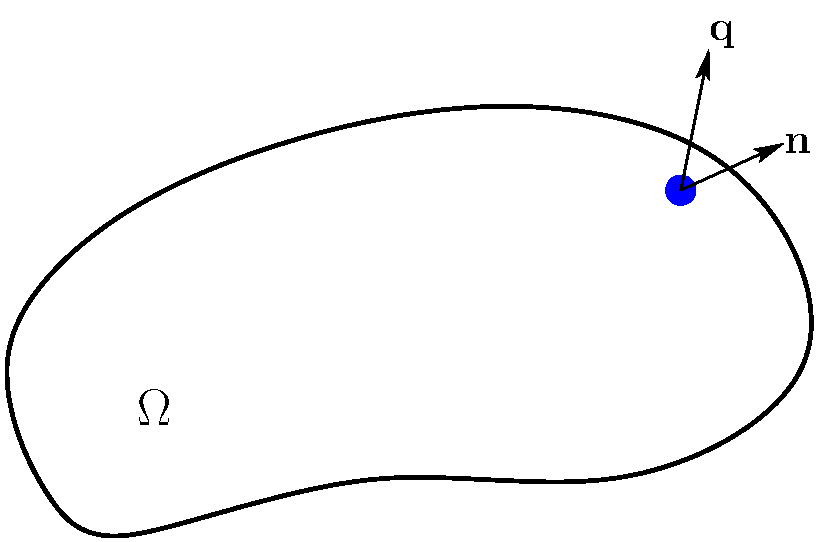
\includegraphics[scale=0.5]{HeatFlux}
  \end{center}
  \caption{
    The domain $\Omega$ and a surface element on the boundary
    $\partial\Omega$. The outward unit normal vector ${\bm n}$ is indicated,
    together with the heat flux ${\bm q}$.
  }
  \label{fig:HeatFlux}
\end{figure}

In the case of constant thermal diffusivity $\kappa$, the governing equation
reduces to the Poisson equation
\begin{align}
  \label{steady-heat}
  - \kappa\nabla^2 u = f.
\end{align}

\section {Unsteady Heat Transfer Problems}

Assuming no fluid flow, energy conservation in the unsteady case is described by
the the unsteady (parabolic) heat equation
\begin{align}
  \label{heat-eq}
  \frac{\partial u}{\partial t}
  = \kappa \nabla^2 u + f \qquad \text{in}\,\Omega.
\end{align}

If we discretize this equation in time using the Euler Backward method, we
obtain
\begin{align}
  \frac{u^{n+1}- u^n}{\Delta t}
  = \kappa\nabla^2 u^{n+1} + f^{n+1},
\end{align}
where superscript $n$ refers to a quantity at time $t^n,\, n=0,1,2,\ldots$. This
can also be expressed as
\begin{align}
  \label{helm-eq}
  \left[- \kappa\nabla^2 +\frac{1}{\Delta t} \right] u^{n+1} =
  \frac{u^n}{\Delta t} + f^{n+1}.
\end{align}
Hence, a typical evolution problem discretized in time using implicit finite
differences will necessitate the solution of a Helmholtz type equation at each
time step. Note that the Helmholtz operator (the operator inside the
parentheses) corresponds to the Laplace operator plus a multiple of the identity
operator.

\section{Eigenvalue problems}

Eigenvalue calculations also form an important application area in science and
engineering. A typical example is the computation of the first eigenmodes or
eigenvibrations in a structure, e.g. a building, a bridge or a turbine. In
order to avoid resonance phenomena in the structure, one can precompute the most
important eigenmodes numerically, and design the structure such that resonance
is avoided for a typical external load or excitation.

To illustrate a typical analysis, consider the following simple model problem:
\begin{align*}
  -\nabla^2 u = \lambda u
\end{align*}
with proper boundary conditions, e.g. the solution specified along the domain
boundary. A numerical model is then constructed for this eigenvalue problem.
This discretization will typically result in a large set of algebraic equations.
The smallest eigenvalues/eigenmodes will give information of \emph{physical
significance}; for our specific model problem, they will approximate the
eigenmodes for a diffusive system and the time constants associated with the
decay of these.

\section{Outputs from partial differential equations}

In many engineering applications, the primary interest may not be the details of
the solution $u$ everywhere in the domain $\Omega$, but rather some very
specific output, e.g. the average temperature over part of the domain boundary,
the drag on an underwater cable due to currents in the sea, or an eigenvalue
(e.g. the lowest eigenfrequency). In these cases, the ultimate interest may
just be a single number. However, in order to compute this output of interest, a
numerical approximation $u_h$ to $u$ needs to be computed on the entire
computational domain $\Omega$, perhaps involving thousands or millions of
unknowns.

\section{Other important issues}

There are many topics that are important in order to successfully obtain
accurate numerical solutions for realistic physical problems.

\subsection{Grid generation}

In this course, we will primarily consider problems in one and two space
dimensions. In one space dimension, the grid generation is trivial. However, for
realistic two and three-dimensional domains, the grid generation itself may pose
a major challenge. In the past, there has been much effort put into the
construction of automatic mesh generators, however, this is still an ongoing
research topic. It turns out that it is easier to decompose a general
computational domain into triangles and tetrahedral elements than it is to
decompose it into quadrilateral or hexahedral elements. This is the main reason
why the use of triangular and tetrahedral (finite) elements tends to be fairly
popular for representing general geometries; e.g. see \autoref{fig:dd_grid}.

\begin{figure}[htbp]
  \begin{center}
    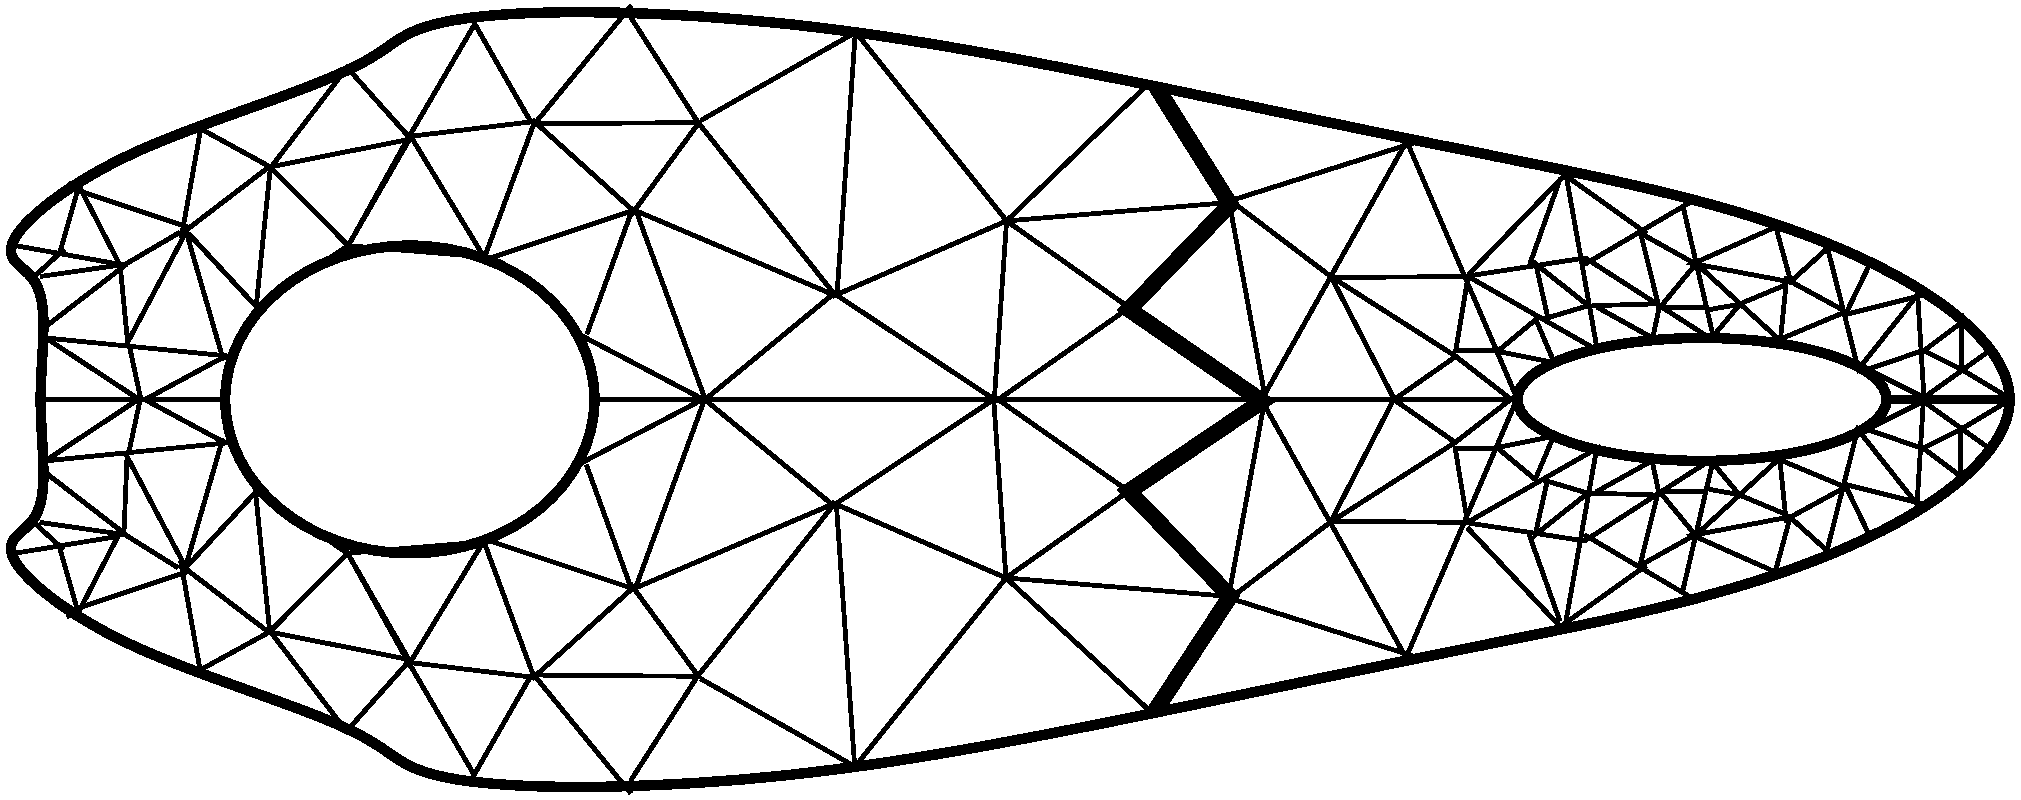
\includegraphics[scale=0.25]{dd_grid}
  \end{center}
  \caption{
    A triangulation of a two-dimensional domains and a partitioning of this
    domain into two subdomains (the bold line represents the subdomain
    interface).
  }
  \label{fig:dd_grid}
\end{figure}

We will not focus on these issues in this course, and stick to simple,
rectangular domains with cartesian meshes.

\subsection{Domain decomposition and parallel computing}

A second important issue related to grid generation is \emph{domain
decomposition}. This is the decompostion of the computational grid into
subdomains, where each subdomain again represents many degrees-of-freedom; see
\autoref{fig:dd_grid}.

Domain decomposition may be important for several reasons. If one is interested
in using a parallel computer with a distributed memory, the global problem
(including the grid) needs to be distributed among the processors. In this
context, each individual subdomain may be associated with a single processor.
However, even on a single process computer, domain decomposition may prove very
useful in the construction of preconditioners for iterative solution methods,
i.e. methods that will speed up the convergence rate when solving the system of
algebraic equations.

Creating a good decomposition from a given grid is not always a trivial task for
general meshes. This is also a field where much progress has been made over the
past few years.

We will come back to this in the course, both in the context of solving the
discretized equation using parallel computers as well as in the context of
preconditioner construction.

\subsection{Adaptivity}

For complex problems, the initial grid is typically generated such that areas
where one expects the solution to exhibit large gradients are well resolved
(i.e. a higher density of elements or degrees-of-freedom is used in those
areas). This approach is very heuristic, and the quality of the underlying mesh
depends strongly on how well one is able to predict the solution structure.

An improved strategy is to use the initial (perhaps coarse) mesh to obtain a
temporary solution which is subsequently used for the purpose of refining the
mesh where the error is expected (or estimated) to be large. This is called
\emph{a posteriori} error estimation and \emph{adaptive} grid refinement (or
perhaps unrefinement). It is an area of considerable research effort since it
promises better error control and reduced computational cost for a fixed error
target. However, adaptive grid refinement is not a trivial task to analyze or to
implement, in particular, for unsteady problems where the solution structure may
change as a function of time.

We will not focus on adaptivity in this course.

\subsection{Visualization}

Once a numerical solution has been computed, the computational results need to
be interpreted. For a multi-dimensional problem, one typically ends up with a
large amount of data. Visualization of these data is often essential in order to
extract useful information from the simulation. Even though the final answer we
are looking for may just be a single number (e.g. the drag), we often want to
understand some of the main features in the solution. With huge amount of data,
visualization (including feature extraction) are invaluable tools. In the
context of parallel computing, visualization is particularly important due to
the very high volume of raw data.

We will consider how to handle the output in this course, but will not focus on
visualization tools. Matlab and Octave will suffice for our needs.

\subsection{Software development}

The effort needed to design and implement a software package for large-scale
simulation of physical systems is typically significant. The associated cost is
therefore also very high. Hence, it is very important to consider good ways to
break down the global problem into smaller modules which can interact in a
flexible and efficient manner.

The use of \emph{object-oriented design} has become popular in recent years. One
of the key issues when designing and implementing a large software package is to
be able to identify commonalities between the various computational tasks, and
to properly encapsulate these so that they may be made into more generic modules
which can be reused for different purposes. An example of this is the solution
of the Poisson equation, which may be used for multiple purposes in the same
simulation package. Another key issue is the concept of data abstraction where
one tries to implement higher-level functionality without necessarily having to
worry about all the details in the lower-level tasks.

\section{Final comments}

It is common to consider the numerical solution of partial differential
equations in the following conceptual model:
\begin{enumerate}
\item we know the computational domain $\Omega$ and the various parameters and
  input data (e.g. the thermal diffusivity $\kappa$ and the volumetric heat
  source $f$);
\item we compute a discrete approximation over the entire domain;
\item we compute the actual output of interest and otherwise interpret and
  visualize the results.
\end{enumerate}

The above approach is often referred to as a \emph{forward problem}, and it may
be sufficient for many problems. However, for certain applications, this mode of
analysis and computation will not suffice. We may not always know the precise
shape of the computational domain, e.g. an airplane wing. In fact, finding the
shape which minimizes the drag may be part of the objective with the simulation.
In such a case, many forward problems are solved, each one hopefully getting
closer to an optimal solution. This type of application represents an example of
an optimization problem. In this context, we note that computing the solution of
a partial differential equation may only give a single data point in a larger
optimization algorithm.

Another area where numerous forward problems may be required is for applications
where the input parameters (e.g. the thermal diffusivity $\kappa$) are not
known, but in fact the quantity of main interest. For such applications, one
will typically have available a certain number of \emph{measurements}
corresponding to multiple \emph{outputs} from the governing equation. The
objective is then to find a distribution of the thermal diffusivity inside the
computational domain such that the difference between the simulated outputs and
the real, physical outputs (or measurements) is minimized. This type of
application represents an example of an \emph{inverse problem}, and is of
significant importance in areas such as medical imaging, estimation of rock
properties etc.

\newcommand{\ub}[1]{{bm #1}}

\chapter{Finite differences for Poisson}

\section{Discretization of equations}

When we want to solve a partial differential equation on a computer, we can
typically only do so in an approximate sense, since a computer can only deal
with a finite amount of data. The process of turning a continuous equation into
a finite-dimensional equation suitable for solving on a computer is referred to
as \emph{discretizing} an equation.

There are several ways to go about this, the most popular being \emph{finite
differences}, \emph{finite elements} and \emph{finite volume} discretizations.
Common to all of these approaches is that at the end of the day, the partial
differential equation is turned into a set of linear equations to solve, i.e.
you end up with something on the form
\[
  \bm A \bm u = bm g
\]
where $\bm A$ is the matrix of linear equations, $\bm u$ is the vector of
unknowns we seek and $\bm g$ is the load (the right hand side in the equation
system).

The simplest and least technical of these are the finite difference approach.
Since this is not a course in numerical solution of partial differential
equations, we will focus on this approach only in this course. But most of what
we consider is also applicable to the other forms of discretization due to the
fact that we will mostly focus on the solution of the linear system of
equations.

\section{Finite difference approximations}

\begin{figure}
  \centering
  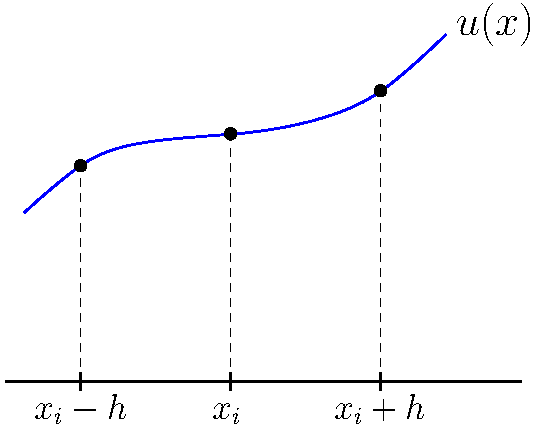
\includegraphics[width=6cm]{FiniteDifference}
  \caption{The function $u(x)$ sampled at a finite difference grid.}
  \label{fig:FiniteDifference}
\end{figure}

Consider the function $u(x)$ depicted in \autoref{fig:FiniteDifference}. A grid
has been introduced---that is, we only consider the function in a discrete sets
of points, $\left\{x_i\right\}_{i=0}^N$, with $x_i = x_0+ih$. Here $h$ is the
grid spacing, here taken as a constant, but in principle we can have a different
spacing between each discrete grid point. We then estimate the derivatives of
this function, only using the values of the function in the discrete sets of
points. This approximation is called a \emph{finite difference}. We now give
alternative finite difference approximations of $u'(x)$ and $u''(x)$ at $x=x_i$.
\begin{align*}
  \intertext{a forward difference approximation:}
  \frac{u(x_i+h)-u(x_i)}{h} &= u'(x_i) + \mathcal{O}(h); \\
  \intertext{two central difference approximations:}
  \frac{u(x_i+h)-u(x_i-h)}{2 h} &= u'(x_i) + \mathcal{O}(h^2), \\ \\
  \frac{u(x_i+h)-2 u(x_i)+u(x_i-h)}{h^2} &= u''(x_i) + \mathcal{O}(h^2).
\end{align*}
The forward difference approximation of $u'(x_i)$ is of first order, meaning
that the error in approximating the first derivative scales linearly with $h$:
if $h$ is reduced by a factor of two, the error is reduced by a factor of two.
The central difference approximations of $u'(x_i)$ and $u''(x_i)$ are of second
order, meaning that the error in approximating the first and second derivatives
scales quadratically with $h$: if $h$ is reduced by a factor of two, the error
is reduced by a factor of four.

We can also generate higher-order approximations to the first and second
derivative of $u(x)$. Higher-order approximations will involve couplings between
more neighboring points.

\section{The one-dimensional Poisson problem}

\subsection{Homogeneous Dirichlet boundary conditions}

We consider here the Poisson equation (or diffusion equation) in one space
dimension,
\begin{align*}
  -u_{xx} = f \qquad \text{in}\,\Omega=(0,1)
\end{align*}
and with homogeneous boundary conditions,
\begin{align*}
  u(0) = u(1) = 0.
\end{align*}

In the following, we will denote the derivative of $u$ with respect to $x$ as
$u_x$, and the second derivative of $u$ with respect to $x$ as $u_{xx}$. This
will prove useful when we later consider two- and three-dimensional problems.

In the Poisson equation, the right hand side $f(x)$ is assumed to be known;
$f(x)$ is often referred to as the source term. In the particular case when
$f=0$, the Poisson equation reduces to the Laplace equation.

In general, the Poisson equation is a partial differential equation (PDE), which
in one space dimension reduces to a standard ordinary differential equation. In
order to obtain a unique solution, we need to specify boundary conditions. In
our case, $u$ is specified at the end points $x=0$ and $x=1$. When $u$ is
specified on the boundary, we say that we have prescribed Dirichlet boundary
conditions. When the prescribed values are zero, as in our case, we say that we
have prescribed homogeneous Dirichlet boundary conditions. The Poisson equation
together with the boundary conditions constitute the Poisson problem.

\begin{figure}
  \centering
  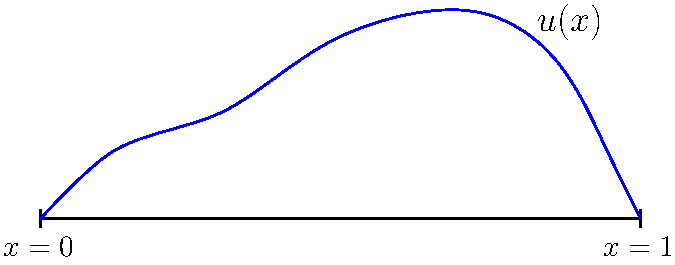
\includegraphics[width=6cm]{Poisson1D_Domain}
  \caption{Domain and solution of the one-dimensional Poisson problem.}
  \label{fig:Poisson1D_Domain}
\end{figure}

\begin{figure}
  \centering
  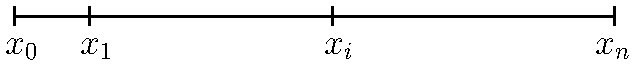
\includegraphics[width=6.5cm]{Poisson1D_Grid}
  \caption{A finite difference grid.}
  \label{fig:Poisson1D_Grid}
\end{figure}

Let $u_i$ be an approximation to $u(x_i)$, $i=1,\ldots,n-1$, and let $f_i =
f(x_i)$. A finite difference approximation of the Poisson problem can then be
expressed as
\begin{align}
  -\left( \frac{u_{i+1} - 2u_i + u_{i-1}}{h^2} \right) &= f_i, \qquad i=1,\ldots,n-1,
  \label{eq:Poisson_int_1d}\\
  u_0 &= 0, \\
  u_{n} &= 0.
\end{align}
We have here $n-1$ unknown values to determine, namely, $u_1, u_2, \ldots,
u_{n-1}$, and we have $n-1$ conditions by requiring that the Poisson equation be
approximated at all the internal grid points $x_1, x_2, \ldots,x_{n-1}$. The
values $u_0$ and $u_{n}$ follow from satisfying the boundary conditions. Note
that we have here used a second order finite difference approximation of
$u_{xx}$.

The equations (\ref{eq:Poisson_int_1d}) can also be expressed as the system
\begin{align*}
  2 u_1 - u_2 &= h^2 f_1, \\
  -u_1 + 2 u_2 - u_3 &= h^2 f_2, \\
  &\vdots \\
  -u_{n-2} + 2 u_{n-1} &= h^2 f_{n-1}.
\end{align*}
We have here already used the fact that $u_0=0$ and $u_{n}=0$.

In matrix form, this system can be expressed as
\begin{align}
 \underbrace{ \begin{pmatrix}
    2 & -1 & & & \\
    -1 & 2 & -1 & & \\
    & & \ddots & & \\
    & & -1 & 2 & -1 \\
    & & & -1 & 2
  \end{pmatrix}
  }_{\bm A}
  \underbrace{ \begin{pmatrix}
    u_1 \\
    u_2 \\
    \vdots \\
    u_{n-2} \\
    u_{n-1}
  \end{pmatrix}
  }_{\bm u}
  &= h^2
  \underbrace{ \begin{pmatrix}
    f_1 \\
    f_2 \\
    \vdots \\
    f_{n-2} \\
    f_{n-1}
  \end{pmatrix}
  }_{\bm f} ,
  \label{eq:A}
\end{align}
or, more succinctly as
\begin{align*}
  \bm A \bm u = \bm g
\end{align*}
where $\bm g = h^2 \bm f$.

It is common to represent the finite difference formula as a stencil, see
\autoref{fig:ThreePointStencil}. By sweeping this across the grid points on our
mesh, it will generate the linear equations given in \eqref{eq:A}.
\begin{figure}
  \centering
  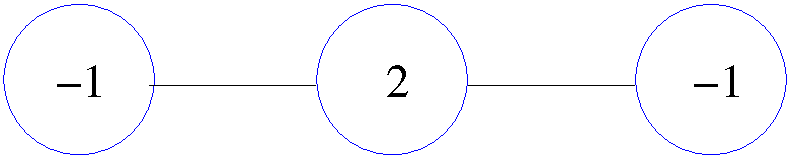
\includegraphics[width=6cm]{ThreePointStencil}
  \caption{
    Weights in the three-point finite difference stencil for the approximation
    of $h^2\cdot$($-u_{xx}$).
  }
  \label{fig:ThreePointStencil}
\end{figure}

We now make some remarks regarding the properties of $\bm A$:
it is a sparse matrix;  more precisely, it is a tridiagonal matrix.
We also note that $\bm A$ is symmetric (i.e., $\bm A = \bm A^\intercal$) and
positive definite (i.e., $\bm v^\intercal \bm A \bm v > 0$ for all vectors $\bm
v \in \mathbb{R}^{n-1}$, $\bm v \not= \bm 0$).

The system of $n-1$ equations is solvable and has a unique solution
\[
  \bm u = \begin{pmatrix} u_1 & u_2 & \cdots & u_{n-1} \end{pmatrix}^\intercal.
\]

The error at the grid points is of second order, i.e.
$|u(x_i)-u_i| \sim \mathcal{O}(h^2)$.

\subsection{Nonhomogeneous Dirichlet boundary conditions}

If $u_0, u_{n} \not= 0$, we can write the $n-1$ equations
\eqref{eq:Poisson_int_1d} as
\begin{align}
  \begin{pmatrix}
    2 & -1 & & & \\
    -1 & 2 & -1 & & \\
    & & \ddots & & \\
    & & -1 & 2 & -1 \\
    & & & -1 & 2
  \end{pmatrix}
  \begin{pmatrix}
    u_1 \\
    u_2 \\
    \vdots \\
    u_{n-2} \\
    u_{n-1}
  \end{pmatrix}
  &= h^2
  \begin{pmatrix}
    f_1 \\
    f_2 \\
    \vdots \\
    f_{n-2} \\
    f_{n-1}
  \end{pmatrix}
  +
  \underbrace{ \begin{pmatrix}
    u_0 \\
    0 \\
    \vdots \\
    0 \\
    u_{n}
  \end{pmatrix}
  }_{\bm b}.
  \label{eq:Poisson1D_DirBC}
\end{align}
This system can again be expressed on the form
\begin{align*}
  \bm A \bm u = \bm g,
\end{align*}
where the left hand side is the same as before. However, the right hand side is
now $\bm g = h^2 \bm f + \bm b$, where the additional vector $\bm b$ is defined
in \eqref{eq:Poisson1D_DirBC}.

\section{Two-dimensional Poisson problem}

We now consider the Poisson problem in a rectangular domain with lengths $L_x$
and $L_y$; see \autoref{fig:Poisson2D_Domain}. The Poisson problem we consider
can be expressed as
\begin{alignat*}{2}
  -\nabla^2 u &= f & \qquad &\text{in}\, \Omega, \\
  u &= 0 & \qquad & \text{on}\, \partial \Omega.
\end{alignat*}
where the right hand side $f(x,y)$ (the source term) is assumed to be known.

\begin{figure}
  \centering
  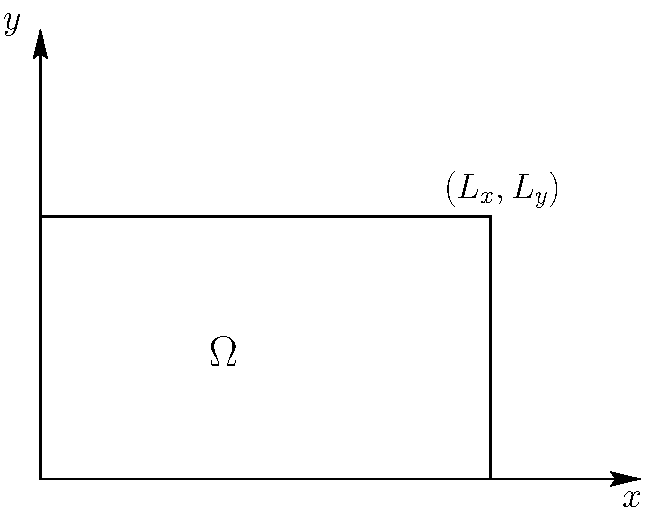
\includegraphics[width=6cm]{Poisson2D_Domain}
  \caption{A rectangular domain for the two-dimensional Poisson problem.}
  \label{fig:Poisson2D_Domain}
\end{figure}

\begin{figure}
  \centering
  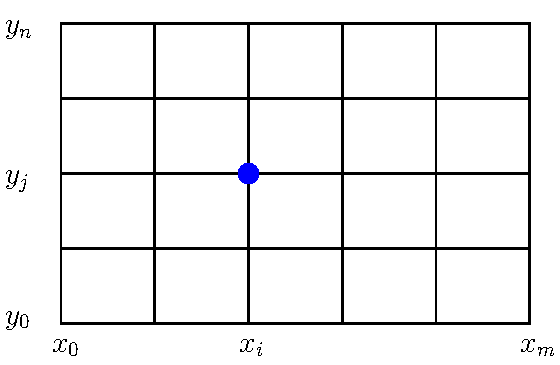
\includegraphics[width=7cm]{Poisson2D_Grid}
  \caption{Finite difference grid: a structured grid.}
  \label{fig:Poisson2D_Grid}
\end{figure}

\subsection{Finite difference discretization}

The finite difference grid points (or nodes) in \autoref{fig:Poisson2D_Grid} are
given by
\begin{align*}
  x_i &= i \cdot h_x, \quad i=0,1,\ldots,m, \qquad h_x = \frac{L_x}{m}, \\
  y_j &= j \cdot h_y, \quad j=0,1,\ldots,n, \qquad h_y = \frac{L_y}{n}.
\end{align*}
Let $u_{i,j}$ be an approximation to $u(x_i,y_j)$, $1\leq i\leq m-1$, $1\leq
j\leq n-1$, and let $f_{i,j} = f(x_i,y_j)$. Then
\begin{align*}
  \frac{u_{i+1,j} - 2 u_{i,j} + u_{i-1,j}}{h_x^2}
  &\simeq \left( \frac{\partial^2 u}{\partial x^2} \right) \biggl|_{(x_i,y_j)} + \mathcal{O}(h_x^2), \\
  \frac{u_{i,j+1} - 2 u_{i,j} + u_{i,j-1}}{h_y^2}
  &\simeq \left( \frac{\partial^2 u}{\partial y^2} \right) \biggl|_{(x_i,y_j)} + \mathcal{O}(h_y^2).
\end{align*}

Assuming (for simplicity) that $m=n$, and that $h_x=h_y=h$, the approximation of
the Poisson problem at the internal grid points can be expressed as
\begin{align*}
  -\frac{(u_{i+1,j}-2u_{i,j}+u_{i-1,j})}{h^2}
  -\frac{(u_{i,j+1}-2u_{i,j}+u_{i,j-1})}{h^2}
  &= f_{i,j}, \qquad i,j=1,\ldots,n-1,
\end{align*}
or
\begin{align}
  -u_{i+1,j}-u_{i-1,j}-u_{i,j+1}-u_{i,j-1}+4u_{i,j} &= h^2 f_{i,j}, \qquad i,j=1,\ldots,n-1.
  \label{eq:Poisson2D_disc}
\end{align}
We note that each unknown value $u_{i,j}$ is coupled to its nearest neighbors
(north, south, east, west) according to the five-point stencil we are using; see
\autoref{fig:FivePointStencil}.

\begin{figure}
  \centering
  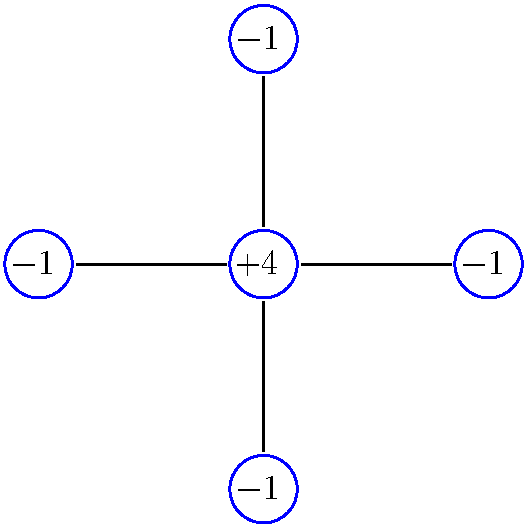
\includegraphics[width=6cm]{FivePointStencil}
  \caption{
    Weights in the five-point finite difference stencil for the approximation of
    $h^2\cdot$($-\nabla^2$).
  }
  \label{fig:FivePointStencil}
\end{figure}

\subsection{Global numbering scheme}

In order to generate a matrix system as in the one-dimensional case, we need to
define a unique ordering of all the degrees-of-freedom. We will here use a
``natural'' ordering in the sense that we number the \emph{internal} nodes along
the $x$-direction first, i.e.
\begin{align*}
  u_{k=(n-1)(j-1)+i} & \equiv u_{i,j} \\
  f_{k=(n-1)(j-1)+i} &\equiv f_{i,j}
\end{align*}
Here, $k = 1,\ldots,N$ with $N=(n-1)^2$. We see that the ordering maps each
node, $(i,j)$, in the grid to a unique, global index, $k$; see
\autoref{fig:NaturalOrdering}.

\begin{figure}
  \centering
  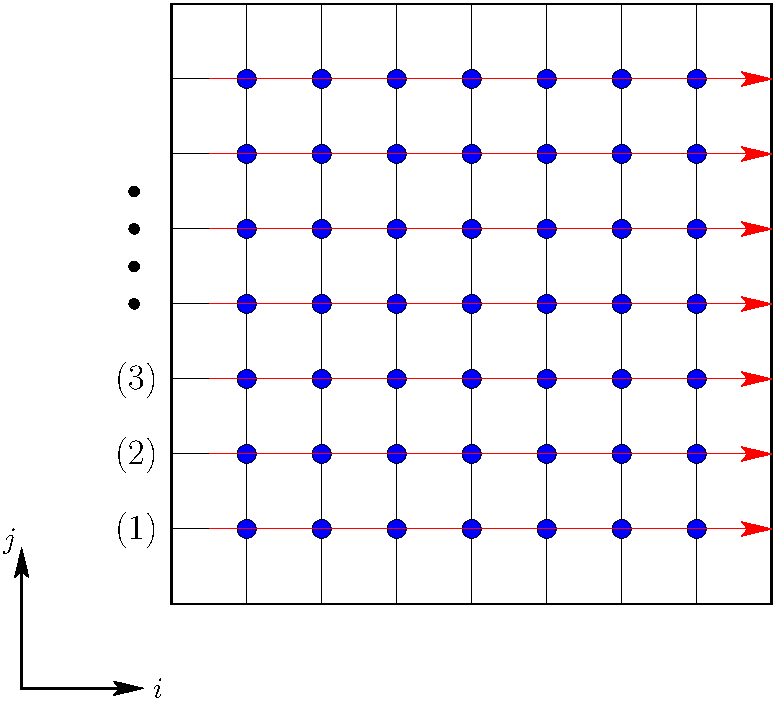
\includegraphics[width=7cm]{NaturalOrdering}
  \caption{
    We use a ``natural'' ordering of the unknowns: we first number all the
    \emph{internal} nodes along ``row'' 1 (in the $x$-direction), followed by
    the nodes in ``row'' 2, etc. The boundary nodes are not counted since these
    values are assumed to be known.
  }
  \label{fig:NaturalOrdering}
\end{figure}

\subsection{System of equations}

With the chosen numbering scheme of the unknowns, we can express the discrete
equations \autoref{eq:Poisson2D_disc} as
\begin{align}
  \bm A \bm u = \bm g,
  \label{eq:Poisson2D_sys}
\end{align}
where the matrix $\underline{A}$ and the vectors $\bm u$ and
$\bm g$ are defined in \autoref{fig:Poisson2D_sys}. The dimension of
this system is $N=(n-1)^2$. The matrix $\bm A$ is still sparse; in particular,
it is pentadiagonal, reflecting the use of a five-point stencil for the
approximation of the Laplace operator. However, while the bandwidth in the
one-dimensional case is one, the bandwidth is now $n$.

Finally, we remark that the matrix $\bm A$ is symmetric and positive definite as
in the one-dimensional case. This will guarantee that the system
\eqref{eq:Poisson2D_sys} is solvable and will yield a unique solution
$\bm u = \begin{pmatrix}u_1&\cdots&u_N\end{pmatrix}^\intercal$. The
discretization error is still quadratic in the grid spacing $h$,
\begin{align*}
  |u(x_i,y_j)-u_{i,j}| \sim \mathcal{O}(h^2). \\
\end{align*}

\begin{figure}
  \centering
  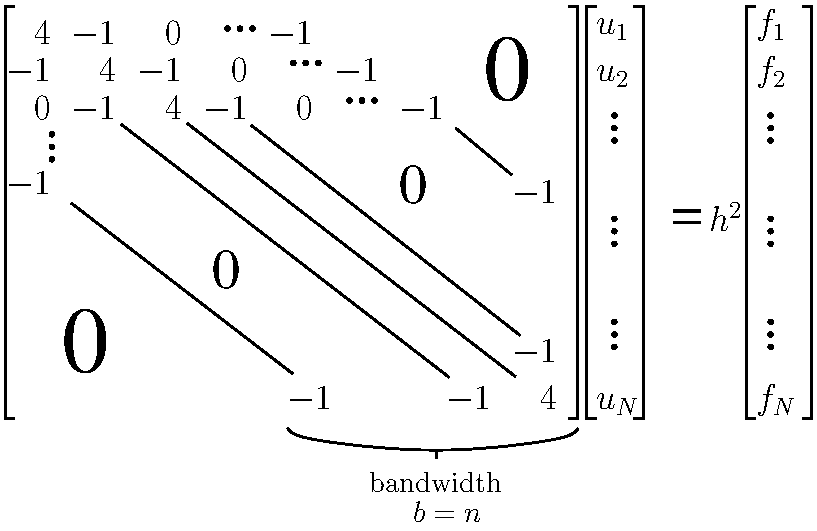
\includegraphics[width=8.5cm]{Poisson2D_System}
  \caption{
    The system of algebraic equations following from the discretization of the
    two-dimensional Poisson problem in a rectangle, and using a ``natural''
    ordering system for the unknowns.
  }
  \label{fig:Poisson2D_sys}
\end{figure}

\subsection{Solution methods for $\bm A \bm u = \bm g$}

Once we have generated the system of equations $\bm A \bm u = \bm g$, we need to
solve this system. There are two main classes of solution methods: direct and
iterative methods. We now give a brief discussion of each of these classes.

\subsubsection{Direct methods}

A direct solution method is method which solves the system of algebraic
equations in a finite, predictable number of steps, e.g., Gaussian elimination,
FFT, etc. This class of the solution methods is often robust, especially when
$\bm A$ is symmetric and positive definite.

In the following, we will use the following notation:
\begin{align*}
  \mathcal{N}_\text{op} &= \text{number of floating-point operations} \\
  \mathcal{M} &= \text{memory requirement (in number of bytes)}
\end{align*}

We will also assume that $\bm A \in \mathbb{R}^{N \times N}$.

As an example, consider full LU-factorization (Gaussian elimination). In this
case, we do not exploit any information about sparsity of $\underline{A}$, but
treat this as a full matrix. For this solution approach, we have
\begin{align*}
  \mathcal{N}_\text{op} &\sim \mathcal{O}(N^3), \\
  \mathcal{M} &\sim \mathcal{O}(N^2).
\end{align*}
Full LU-factorization is robust and easy to use, however the cost does not scale
very well since we need $\mathcal{O}(N^2)$ operations per unknown. For large
systems, this cost becomes prohibitive.

A better approach is to exploit the banded structure of $\bm A$; see
\autoref{fig:Banded}. For a banded LU-factorization, we have
\begin{align*}
  \mathcal{N}_\text{op} &\sim \mathcal{O}(N b^2) ,\\
  \mathcal{M} &\sim \mathcal{O}(N b) .
\end{align*}

\begin{figure}
  \centering
  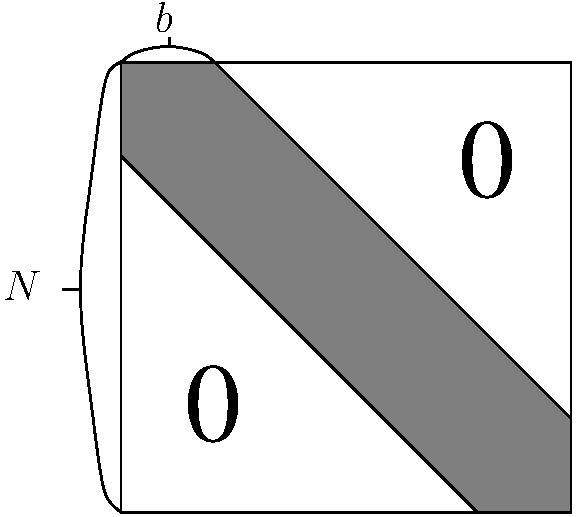
\includegraphics[width=6cm]{BandedMatrix}
  \caption{
    A banded matrix with band width $b$. In the context of solving partial
    differential equations numerically, we often have $b \ll N$.
  }
  \label{fig:Banded}
\end{figure}

We remark that, since $\bm A$ is symmetric and positive definite, no pivoting is
necessary during the Gaussian elimination process.

\begin{figure}
  \centering
  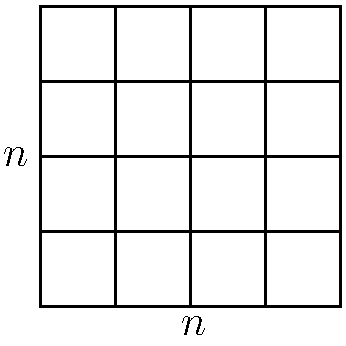
\includegraphics[width=4cm]{Poisson2D_ntimesnGrid}
  \caption{
    The two-dimensional grid associated with the finite difference solution of
    the Poisson problem. Here, $N \sim n^2$, while the bandwidth of
    $\bm A$ using a natural numbering scheme is $b\sim n$.
  }
  \label{fig:Poisson_nxn}
\end{figure}

Let us now revisit \eqref{eq:Poisson2D_sys} which we arrived at based on a
finite difference discretization of the two-dimensional Poisson problem. If we
exploit the banded structure of $\bm A$ during the LU-factorization, see
\autoref{fig:Poisson_nxn}, the cost of this method is
\begin{align*}
  \mathcal{N}_\text{op} &\sim \mathcal{O}(N b^2)
                          \sim \mathcal{O}(n^4) \sim \mathcal{O}(N^2)\\
  \mathcal{M} &\sim \mathcal{O}(N b) \sim \mathcal{O}(n^3) \sim \mathcal{O}(N^{3/2})
\end{align*}

However, if we instead use FFT (The Fast Fourier Transform), as we will discuss
later, the cost of solving \eqref{eq:Poisson2D_sys} is only
\begin{align*}
  \mathcal{N}_{op} &\sim \mathcal{O}(N \log N), \\
  \mathcal{M} &\sim \mathcal{O}(N).
\end{align*}
This is approximately optimal since the computational cost is $\mathcal{O}(\log
N)$ per unknown, and the memory requirement is constant per unknown, independent
of the value of $N$.

\subsubsection{Iterative methods}

An iterative method will give a new estimate or update of the solution at each
iteration. In most cases, the exact solution to $\bm A \bm u = \bm g$ will never
be reached. However, one can get as close as one wishes, but this may require
many iterations and imply a high computational cost. Unlike a direct method, the
solution is not reached after a finite, predictable number of floating point
operations. In order to stop the iteration, a stop criterion has to be specified
by the user. This can be some kind of tolerance, e.g. that the residual (i.e.
the difference between the left hand side and the right hand side of the
equation system) is less than a tolerance. Typically, when the tolerance is
reduced, the number of iterations increases.

Another aspect with iterative methods is that the computational cost can be
problem dependent; see \autoref{fig:Poisson_aspect}. This is different from
direct solution methods which often only depends on the problem size, $N$.

\begin{figure}
  \centering
  
\includegraphics[height=0.2\textwidth]{Poisson2D_aspect1} \\
  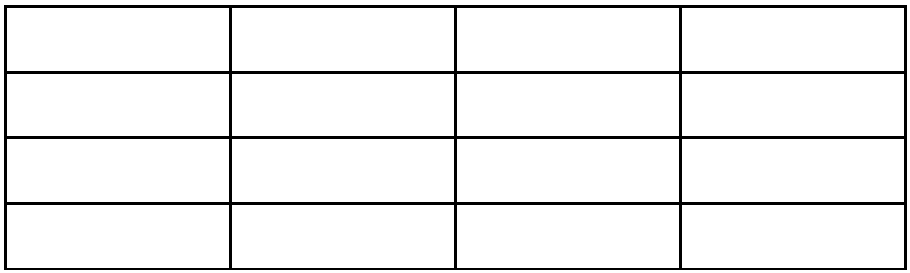
\includegraphics[height=0.2\textwidth]{Poisson2D_aspect2}
  \caption{
    Two different computational domains for the Poisson problem, but with the
    same number of unknowns after discretization. The problem size, $N$, is
    therefore the same. The number of iterations required to solve the system of
    algebraic equations will depend on the aspect ratio (the ratio $L_x/L_y$) of
    the domains. Hence, the computational cost for solving the problem on the
    right will be higher than for the problem on the left. This is in contrast
    to a direct method where the computational cost for solving the two systems
    will be the same.
  }
  \label{fig:Poisson_aspect}
\end{figure}

A great advantage of many iterative methods is that they often have a
\emph{scalable} memory requirement, i.e. that the memory requirement is
proportional to $N$ and not some power of $N$.

Another characteristics with iterative methods is that much of the computational
cost is related to performing basic linear algebra operations such as
matrix-vector products, inner products, etc.

Finally, we remark that iterative methods are very suitable for parallel
processing, and are often the only viable alternative for large,
three-dimensional problems.

Some examples of iterations methods suitable for symmetric and positive definite
problems are: Jacobi iteration, Gauss-Seidel iteration, the conjugate gradient
method, and multigrid methods (where the last two methods are commonly used
today).

\chapter{Diagonalization for Poisson}

\section{Direct method based on diagonalization}

Let us now consider a different way of solving the finite difference equations
we derived in the context of discretizing the Poisson problem. The method is
based on \emph{diagonalization}, and we first explain the approach in the context
of the one-dimensional Poisson problem:

\begin{align*}
  -u_{xx} &= f \quad \text{in}\, \Omega = (0,1), \\
  u(0) = u(1) &= 0.
\end{align*}
Assume that we use a uniform finite difference grid given by:
\begin{equation*}
  x_i = x_0 + ih, \quad i=0,1,\ldots,n.
\end{equation*}

The corresponding system of algebraic equations can be written as
\begin{align*}
  \frac{1}{h^2}
  \begin{pmatrix}
    2 & -1 & & & \\
    -1 & 2 & -1 & & \\
    & -1 & 2 & -1 & \\
    & & & \ddots & -1 \\
    & & & -1 & 2
  \end{pmatrix}
  \begin{pmatrix}
    u_1 \\
    u_2 \\
    \vdots \\
    u_{n-1}
  \end{pmatrix}
  =
  \begin{pmatrix}
    f_1 \\
    f_2 \\
    \vdots \\
    f_{n-1}
  \end{pmatrix},
\end{align*}
where $u_i$ is an approximation to $u(x_i) = u(ih),$ $i=1,\ldots,n-1$,
$f_i=f(x_i)$, and $u_0 = u_n = 0$ due to the specified boundary conditions. Let
us write this system as

\begin{align*}
  \frac{1}{h^2} \bm T \bm u = \bm f
\end{align*}
where
\begin{align*}
  \bm T =
  \begin{pmatrix}
    2 & -1 & & & \\
    -1 & 2 & -1 & & \\
    & -1 & 2 & -1 & \\
    & & & \ddots & -1 \\
    & & & -1 & 2
  \end{pmatrix} , \qquad
  \bm u =
  \begin{pmatrix}
    u_1 \\
    \vdots \\
    u_{n-1}
  \end{pmatrix} , \qquad
  \bm f =
  \begin{pmatrix}
    f_1 \\
    \vdots \\
    f_{n-1}
  \end{pmatrix},
\end{align*}
and $h$ is the grid size or mesh size. Since $\bm T$ is symmetric
positive definite, it can be \emph{diagonalized}.

\subsection{Diagonalization of $\bm T$}

Diagonalization of $\bm T$ means that we wish to find the eigenvalues
$\lambda_j$ and the eigenvectors $\bm q_j$ of $\bm T$,
\begin{align*}
  \bm T \bm q_j &= \lambda_j \bm q_j \quad j=1,\ldots,n-1,
\end{align*}
where
\begin{align*}
  \lambda_j &> 0 \qquad &\text{(positive eigenvalues)}, \\
  \bm q_k^\intercal \bm q_j &= \delta_{jk} \qquad &\text{(orthonormal eigenvectors)}.
\end{align*}

We collect all the eigenvectors $\bm q_j$ into the orthogonal matrix $\bm Q$,
\begin{equation*}
  \bm Q = \begin{pmatrix} \bm q_1 & \bm q_2 & \cdots & \bm q_{n-1}\end{pmatrix}.
\end{equation*}
Then
\begin{align*}
  \bm T \bm Q &= \bm Q \bm \Lambda
\end{align*}
where
\begin{align*}
  \bm Lambda &= \operatorname{diag}(\lambda_1, \ldots, \lambda_{n-1}) =
  \begin{pmatrix}
    \lambda_1 & & \\
     & \ddots & \\
    & & \lambda_{n-1}
  \end{pmatrix}.
\end{align*}
Since
\begin{align*}
  \bm Q^\intercal \bm Q = \bm I =
  \begin{pmatrix}
    1 & & \\
    & \ddots & \\
    & & 1
  \end{pmatrix} \qquad
  \Rightarrow \quad \bm Q^\intercal = \bm Q^{-1},
\end{align*}
and
\begin{align}
  \bm T &= \bm Q \bm \Lambda \bm Q^\intercal
  \label{eq:T_diag}
\end{align}
or
\begin{align*}
  \bm Q^\intercal \bm T \bm Q = \bm \Lambda \qquad \text{(diagonal)}.
\end{align*}

Following this approach the finite difference approximation can be computed as
follows:
\begin{alignat*}{2}
  \bm g &\equiv  h^2 \bm f \quad &  \qquad \qquad \bm g
  &: \; \mathcal{O}(n) ~ \text{operations} \\
  \\
  \bm T \, \bm u &= \bm g \\
  \bm Q \, \bm \Lambda \, \bm Q^T \bm u &= \bm g \\
  \bm \Lambda \underbrace{\bm Q^\intercal \bm u}_{\tilde{\bm u}}
  &= \underbrace{\bm Q^\intercal \bm g}_{\tilde{\bm g}}
  & \tilde{\bm g} &: \; \mathcal{O}(n^2) ~ \text{operations} \\
  \\
  \bm \Lambda \tilde{\bm u} &= \tilde{\bm g} \\
  \tilde{\bm u} &= \bm \Lambda^{-1} \tilde{\bm g}
  & \tilde{\bm u} &: \; \mathcal{O}(n) ~ \text{operations} \\
  \\
  \bm Q^T \bm u &= \tilde{\bm u} \\
  \bm u &= \bm Q \tilde{\bm u} & \bm u
  &: \; \mathcal{O}(n^2) ~ \text{operations}
\end{alignat*}
Note that the transformations
\begin{equation*}
  \tilde{\bm g} = \bm Q^\intercal \bm g \quad \text{and} \quad \bm u = \bm Q \tilde{\bm u}
\end{equation*}
are \emph{matrix-vector products}. In summary, we can compute $\bm u$ in
\begin{equation*}
  \mathcal{O}(n) + \mathcal{O}(n^2) + \mathcal{O}(n) + \mathcal{O}(n^2)
  \sim \mathcal{O}(n^2) ~ \text{floating-point operations}.
\end{equation*}
Hence, we can solve our finite difference system in $(n-1)$ unknowns in
$\mathcal{O}(n^2)$ operations. This is \emph{not} competitive with a direct
solution algorithm based upon LU-factorization (Gaussian elimination) of a
tridiagonal matrix, which can be done in $\mathcal{O}(n)$ operations (since the
bandwidth is equal to one).

Let us also compare the memory requirement:
\begin{align*}
  &\mathcal{O}(n^2) ~\text{for the diagonalization approach
  (we need to store $\bm Q$)}; \\
  &\mathcal{O}(n) ~\text{for a tridiagonal direct solver}.
\end{align*}
Again, the diagonalization approach is {\em not} competitive.

So, why bother? The answer is that the diagonalization approach becomes more
interesting in $\mathbb{R}^2$. In addition, we will later see how we can use the
Fast Fourier Transform (FFT) to lower the computational complexity.

\section{The Poisson problem in $\mathbb{R}^2$}

The two-dimensional Poisson problem on the unit square is given by

\begin{equation}
  \begin{split}
    -\nabla^2 u &= f \qquad \text{in} ~ \Omega=(0,1) \times (0,1), \\
    u &= 0 \qquad \text{on} ~ \partial \Omega, \\
  \end{split}
  \label{eq:Poisson2D}
\end{equation}
where
\[
  \nabla^2 u = \frac{\partial^2 u}{\partial x^2}
  + \frac{\partial^2 u}{\partial y^2}.
\]

\begin{figure}
  \centering
  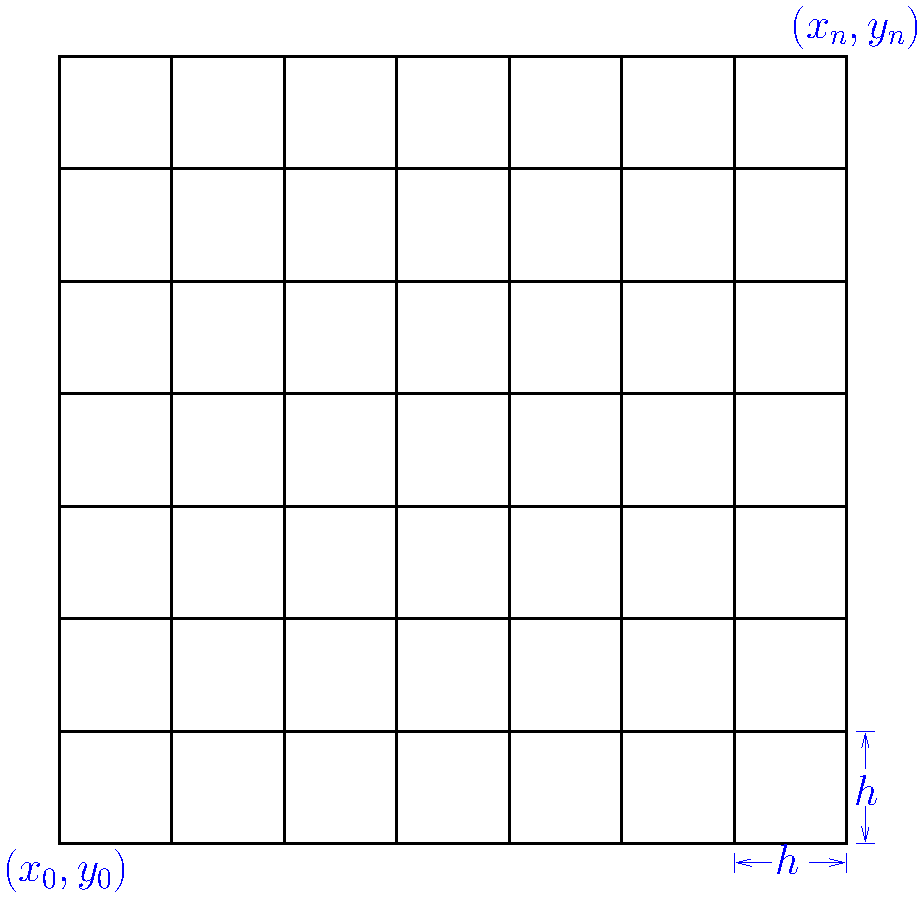
\includegraphics[width=8cm]{FiniteDifferenceGrid}
    \caption{A uniform finite difference grid.}
  \label{fig:FDM_grid_2D}
\end{figure}

Again, using the notation $u_{i,j} \simeq u(x_i,y_j) = u(i h, j h)$ and
$f_{i,j}=f(x_i,y_j)$, and discretizing \eqref{eq:Poisson2D} using the 5-point
stencil (see Figure \ref{fig:FDM_grid_2D}), the discrete equations read
\begin{equation}
  -\frac{(u_{i+1,j}-2u_{i,j}+u_{i-1,j})}{h^2} - \frac{(u_{i,j+1}-2u_{i,j}+u_{i,j-1})}{h^2} = f_{i,j}
  \label{eq:FDM_sys}
\end{equation}
for $1 \leq i,j \leq n-1$.

\subsection{Diagonalization}

Let
\begin{equation*}
  \bm U =
  \begin{pmatrix}
    u_{1,1} & \cdots & u_{1,n-1} \\
    \vdots & \ddots & \vdots \\
    u_{n-1,1} & \cdots & u_{n-1,n-1}
  \end{pmatrix}
\end{equation*}
and
\begin{equation*}
  \bm T =
  \begin{pmatrix}
    2 & -1 & & & \\
    -1 & 2 & -1 & & \\
    & & \ddots & & \\
    & & -1 & 2 & -1 \\
    & & & -1 & 2
  \end{pmatrix}.
\end{equation*}

Then,
\begin{alignat*}{2}
  (\bm T \bm U)_{ij} &= 2u_{i,j} - u_{i+1,j}, & \qquad i=1, \\
  (\bm T \bm U)_{ij} &= -u_{i-1,j}+2u_{i,j} - u_{i+1,j}, &\qquad 2 \leq i \leq n-2, \\
  (\bm T \bm U)_{ij} &= -u_{i-1,j}+2u_{i,j}, &\qquad i=n-1.
\end{alignat*}
and thus,
\begin{equation}
  \frac{1}{h^2} (\bm T \bm U)_{ij} \simeq
  - \left( \frac{\partial^2 u}{\partial x^2} \right)_{i,j}.
\end{equation}

Similarly in the other direction,
\begin{equation}
  \frac{1}{h^2} (\bm U \bm T)_{ij} \simeq
  - \left( \frac{\partial^2 u}{\partial y^2} \right)_{i,j}.
\end{equation}

Our finite difference system (\ref{eq:FDM_sys}) can thus be expressed as
\begin{equation*}
  \frac{1}{h^2} (\bm T \bm U + \bm U \bm T)_{ij} = f_{i,j}
  \qquad \text{for} \qquad 1 \leq i,j \leq n-1, \\
\end{equation*}
or
\begin{equation}
  \bm T \bm U + \bm U \bm T = \bm G
  \label{eq:Poisson2D_TUUT}
\end{equation}
where
\begin{equation*}
  \bm G = h^2
  \begin{pmatrix}
    f_{1,1} & \ldots & f_{1,n-1} \\
    \vdots & \ddots & \vdots \\
    f_{n-1,1} & \ldots & f_{n-1,n-1}
  \end{pmatrix}.
\end{equation*}

Combining \eqref{eq:T_diag} and \eqref{eq:Poisson2D_TUUT} we get
\begin{equation}
  \bm Q \bm \Lambda \bm Q^\intercal \bm U + \bm U \bm Q \bm \Lambda \bm Q^\intercal = \bm {G}.
  \label{eq:Poisson2D_T_diag}
\end{equation}

Multiplying \eqref{eq:Poisson2D_T_diag} from the right with $\bm Q$ and from the
left with $\bm Q^T$, and using the fact that $\bm Q^\intercal \bm Q = \bm I$, we
get
\begin{equation*}
  \bm \Lambda \underbrace{\bm Q^\intercal \bm U \bm Q}_{\tilde{\bm U}} +
  \underbrace{\bm Q^\intercal \bm U \bm Q}_{\tilde{\bm U}} \bm \Lambda =
  \underbrace{\bm Q^\intercal \bm G \bm Q}_{\tilde{\bm G}}.
\end{equation*}

Hence, (\ref{eq:Poisson2D_TUUT}) may be solved in three steps:

\begin{enumerate}
\item Compute $\tilde{\bm G}$ using matrix-matrix products
  \begin{equation*}
    \tilde{\bm G} = \bm Q^\intercal \bm G \bm Q.
  \end{equation*}
\item Solve for $\tilde{\bm U}$.
  \begin{align*}
    \bm \Lambda \tilde{\bm U} + \tilde{\bm U} \bm \Lambda &= \tilde{\bm G} \\
    \lambda_i \tilde{u}_{ij} + \tilde{u}_{ij} \lambda_j &= \tilde{g}_{ij} \\
    \tilde{u}_{ij} &= \frac{\tilde{g}_{ij}}{\lambda_i + \lambda_j}
  \end{align*}
\item Compute $\bm U$ using matrix-matrix products
  \begin{equation*}
    \bm U = \bm Q \tilde{\bm U} \bm Q^\intercal
  \end{equation*}
\end{enumerate}

Here,
\begin{equation*}
  \bm U, \tilde{\bm U}, \tilde{\bm G}, \bm Q \in \mathbb{R}^{(n-1) \times (n-1)}
\end{equation*}

\subsubsection{Computational cost}

The number of degrees of freedom (or unknowns) $N$ is
\begin{align*}
N = (n-1)^2 \sim \mathcal{O}(n^2) \quad (n \gg 1).\\
\end{align*}

\begin{enumerate}
\item Two matrix-matrix products give $\mathcal{O}(n^3)$ operations.
\item $\mathcal{O}(n^2)$ scalar constant time operations give $\mathcal{O}(n^2)$.
\item Two matrix-matrix products give $\mathcal{O}(n^3)$ operations.
\end{enumerate}
In summary, we can compute the discrete solution, $\bm U$, in
$\mathcal{O}(n^3)=\mathcal{O}(N^{3/2})$ operations.

Note: this method is an example of a {\em direct method}.

\subsubsection{Comparison with other direct methods}

\begin{table}
    \caption{
      Computational cost and memory requirement for three different
      direct methods. The number of unknowns is $N=\mathcal{O}(n^2)$. For the
      banded solver, we have used a bandwidth $b \sim \mathcal{O}(n)$. Full LU
      means LU-factorization without exploiting sparsity.
    }
    \label{tab:DirectMethods_ComputationalCost}
  \begin{center}
    \bgroup\def\arraystretch{1.2}
    \begin{tabular}{lrr}
      \hline
      Method & Operations ($\mathcal{N}_\text{op}$) & Memory requirement ($\mathcal{M}$) \\
      \hhline{===}
      Diagonalization & $\mathcal{O}(N^{3/2}) = \mathcal{O}(n^3)$ & $\mathcal{O}(N) = \mathcal{O}(n^2)$ \\
      Banded LU & $\mathcal{O}(N b^2) = \mathcal{O}(n^4)$ & $\mathcal{O}(Nb) = \mathcal{O}(n^3)$ \\
      Full LU & $\mathcal{O}(N^3) = \mathcal{O}(n^6)$ & $\mathcal{O}(N^2) = \mathcal{O}(n^4)$ \\
      \hline
    \end{tabular}
    \egroup
  \end{center}
\end{table}

We conclude that the diagonalization method is much more attractive in
$\mathbb{R}^2$ than in $\mathbb{R}^1$. The number of floating-point operations
per degree of freedom is $\mathcal{O}(n)$, while the memory requirement is close
to optimal (i.e. scalable).

\subsubsection{The matrices $\bm Q$ and $\bm \Lambda$}

The computational cost associated with the diagonalization approach tacitly
assumes that we know the eigenvector matrix $\bm Q$ and the corresponding
eigenvalues. Let us therefore derive explicit expressions for these. To this
end, consider first the continuous eigenvalue problem
\begin{equation*}
  \begin{split}
    -u_{xx} &= \lambda u \qquad \qquad \text{in } \Omega=(0,1), \\
    u(0) = u(1) &= 0,
  \end{split}
\end{equation*}
with solutions
\begin{equation*}
  \begin{split}
    \bar{u}_j(x) &= \sin(j \pi x), \\
    \bar{\lambda}_j &= j^2 \pi^2,
  \end{split}
  \qquad j=1,2,\ldots,\infty.
\end{equation*}

Consider now the discrete eigenvalue problem
\begin{equation*}
  \bm T \tilde{\bm q}_j =
  \lambda_j \tilde{\bm q}_j
\end{equation*}
Try eigenvector solutions which correspond to the continuous eigenfunctions
$\bar{u}_j(x)$ sampled at the grid points $x_i, i=1,\ldots,n-1$, i.e.
\begin{equation*}
  \begin{split}
    (\tilde{\bm q}_j)_i &= \bar{u}_j (x_i) \\
    &= \sin(j \pi x_i) \\
    &= \sin(j \pi (i h)), \\
    &= \sin \left(\frac{i j \pi}{n} \right)
  \end{split}
\end{equation*}

Operating on $\tilde{\bm q}_j$ with $\bm T$ gives
\begin{equation*}
  (\bm T \tilde{\bm q}_j)_i =
  \underbrace{2\left( 1 - \cos\left( \frac{j\pi}{n} \right) \right)}_{\lambda_j}
  \underbrace{\sin\left( \frac{i j \pi}{n} \right)}_{(\tilde{\bm q}_j)_i}
\end{equation*}

Hence, our try was successful: operating on $\tilde{\bm q}_j$ with $\bm T$ gives
a multiple of $\tilde{\bm q}_j$.

In order to proceed, set $\bm q_j = \alpha \tilde{\bm q}_j$, and choose $\alpha$
such that $\bm q_j$ is normalized:

\begin{align*}
  (\bm q_j)_i &= \sqrt{\frac{2}{n}} \sin \left( \frac{ij \pi}{n} \right),
                \qquad \qquad 1 \leq i,j \leq n-1, \\
  \lambda_j &= 2 \left( 1 - \cos \left( \frac{j \pi}{n} \right) \right).
\end{align*}

For ${j \ll n}$, we observe that
\begin{align*}
  \lambda_j
  &\simeq 2 \left( 1 - \left( 1 -\frac{1}{2} \frac{j^2 \pi^2}{n^2} + \ldots \right) \right)
    \simeq \frac{j^2 \pi^2}{n^2}. \\
  \intertext{Since $h=1/n$, we have}
  \lambda_j &\simeq h^2j^2 \pi^2 = h^2 \bar{\lambda}_j \qquad \text{ for } j \ll n.
\end{align*}

Since the approximation of the one-dimensional Laplace operator on our finite
difference grid is equal to $\bm T / h^2$, this is the same as saying that the
first, lowest eigenvalues (and eigenvectors) for the continuous case are well
approximated by our finite difference formulation.

Note that
\begin{align*}
 \bm Q_{ij}
  &= (\bm q_j)_i = \sqrt{\frac{2}{n}} \sin \left( \frac{ij \pi}{n} \right),
    \qquad 1 \leq i,j \leq n-1, \\
\end{align*}
and that indeed
\begin{align*}
  \bm Q^\intercal = \bm Q, \qquad \bm Q^\intercal \bm Q = \bm I.
\end{align*}

From the comparison of the computational cost shown earlier, the diagonalization
approach to solving the discrete Poisson problem appears promising.

\textbf{Questions}:
\begin{enumerate}
\item Can the matrix-matrix multiplications be done fast?
\item Can the matrix-matrix multiplications be parallelized?
\item Can we do better?
\end{enumerate}

\subsubsection{Numerical results}

A diagonalization solver based on ``standard'' matrix-matrix product code (i.e.
no special library was used). The code was run on a PC, Pentium III with 512 MB
RAM (2000) and on a single processor on Gridur, MIPS R14000 with 1 GM RAM
(2006).

We define $\tau(n)$ as the total simulation time (in seconds), $\tau_1(n) =
\tau(n)/n^2$ as the time spent per degree of freedom, and
\[
  r(n) = \frac{\tau_1(n)}{\tau_1(n/2)}
\]
as the slowdown factor when doubling the problem size.

See \autoref{tbl:numres-diag}. The source code follows.

\begin{table}
  \caption{
    Simulation results for the numerical approximation of the two-dimensional
    Poisson equation by finite differences. The solution of the system of
    discrete equations is based on diagonalization techniques and matrix-matrix
    products. A listing of the FORTRAN program used in these tests is given
    below. It is interesting to note that the elapsed time on a single processor
    on Gridur is reduced by a factor of more than 80 compared to using the PC
    from 2000 when $n=1024$.
  }
  \label{tbl:numres-diag}
  \begin{center}
    \bgroup\def\arraystretch{1.2}
    \begin{tabular}{r|lll|ll}
      \hline
      \multicolumn{1}{r}{}
      & \multicolumn{3}{|c|}{PC (2000)}
      & \multicolumn{2}{c}{Gridur (2006)} \\
      \hline
      $n$ & $\tau(n)$ & $\tau_1(n)$ & $r(n)$ & $\tau(n)$ & $\tau_1(n)$ \\
      \hhline{======}
      $32$ & $1.80 \cdot 10^{-2}$ & $1.76 \cdot 10^{-5}$ & & &\\
      $64$ & $1.50 \cdot 10^{-1}$ & $3.66 \cdot 10^{-5}$ & $2.1$ & & \\
      $128$ & $1.20$ & $7.34 \cdot 10^{-5}$ & $2.0$ & $2.45 \cdot 10^{-2}$ & $1.50 \cdot 10^{-6}$ \\
      $256$ & $9.84$ & $1.50 \cdot 10^{-4}$ & $2.0$ & $0.167$ & $2.55 \cdot 10^{-6}$ \\
      $512$ & $103.9$ & $3.96 \cdot 10^{-4}$ & $2.6$ & $1.33$ & $5.08 \cdot 10^{-6}$ \\
      $1024$ & $873.2$ & $8.33 \cdot 10^{-4}$ & $2.1$ & $10.33$ & $9.85 \cdot 10^{-6}$ \\
      \hline
      & $\sim \mathcal{O}(n^3)$ & $\sim \mathcal{O}(n)$ & & & \\
      \hline
    \end{tabular}
    \egroup
  \end{center}
\end{table}

\begin{lstlisting}[style=fortran]
  program poisson

  ! Program to solve the two-dimensional Poisson equation on
  ! a unit square using one-dimensional eigenvalue decompositions
  ! and matrix-vector products.
  ! In this example, the right hand side f=1.

  ! Einar M. Ronquist
  ! NTNU, October 2000

  parameter (n = 256)
  parameter (m = n-1)

  real*8 diag(m), q(m,m), qt(m,m), b(m,m), u(m,m), w(m,m), pi
  real*4 tarray(2), t1, t2, dt

  t1 = etime(tarray)

  h  = 1./n
  pi = 4.*atan(1.)

  do i=1,m
    diag(i) = 2*(1-cos(i*pi/n))
  enddo

  do j=1,m
    do i=1,m
      q(i,j) = sin(i*j*pi/n) * sqrt((2./n))
    enddo
  enddo

  do j=1,m
    do i=1,m
      qt(i,j) = q(j,i)
    enddo
  enddo

  do j=1,m
    do i=1,m
      b(i,j) = h*h
    enddo
  enddo

  call mxm(b,m,q,m,w,m)
  call mxm(qt,m,w,m,b,m)

  do j=1,m
    do i=1,m
      u(i,j) = b(i,j)/(diag(i)+diag(j))
    enddo
  enddo

  call mxm(u,m,qt,m,w,m)
  call mxm(q,m,w,m,u,m)

  t2 = etime(tarray)
  dt = t2-t1
  write(6,*) ' '
  write(6,*) 'dt (total)= ',dt
  dt = dt/(n*n)
  write(6,*) 'dt (per dof)= ',dt

  stop
  end

  subroutine mxm (a,n1,b,n2,c,n3)

  ! matrix-matrix product c = a*b

  real*8 a(n1,n2), b(n2,n3), c(n1,n3)
  do j=1,n3
    do i=1,n1
      c(i,j) = 0.0
      do k=1,n2
        c(i,j) = c(i,j) + a(i,k)*b(k,j)
      enddo
    enddo
  enddo

  return
  end
\end{lstlisting}

\subsection{Fast diagonalization methods}

The most expensive operation in the diagonalization method introduced in the
previous section is of the type
\begin{align*}
  \bm v^* &= \bm Q \bm v = \bm Q^\intercal \bm v, \\
  \intertext{where}
  Q_{ij} &= \sqrt{\frac{2}{n}} \sin \left( \frac{ij \pi}{n} \right) \qquad \qquad 1 \leq i,j \leq n-1.
\end{align*}

We will now consider ways to obtain $\bm v^*$ in $\mathcal{O}(n \log n)$
operations instead of $\mathcal{O}(n^2)$.

\subsubsection{Discrete Fourier Transform (DFT)}

Consider a periodic function $v(x)$ with period $2 \pi$. Consider sampling this
function at the equidistant points $x_j$, $j=0,1,\ldots,N$ with $x_j=j h$,
$\quad h=2 \pi / N$. Let $v_j = v(x_j) = v(j h)$, $j=0,1,\ldots,N$.
\begin{figure}[h]
  \centering
  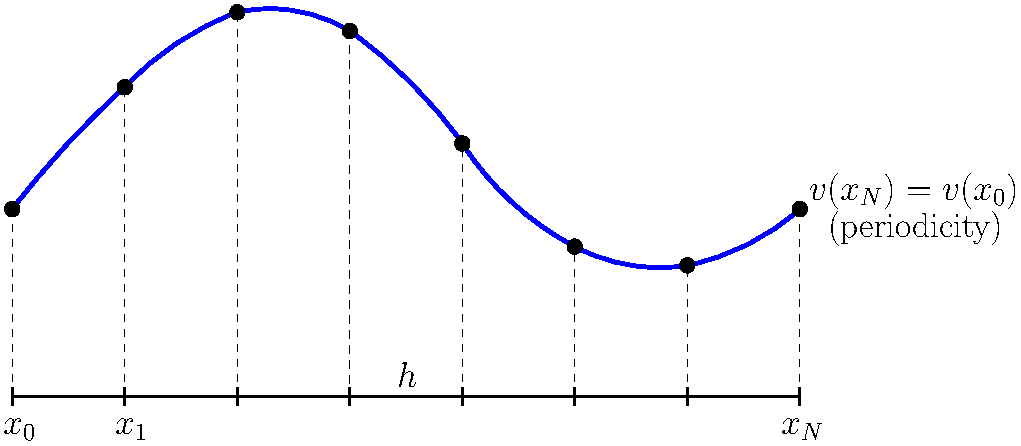
\includegraphics[width=10cm]{PeriodicFunction}
\end{figure}

Consider the vectors $\bm \varphi_k$, where
\begin{equation*}
  (\bm \varphi_k)_j = \text{e}^{\text{i} k x_j}, \qquad j,k=0,1,\ldots,N-1.
\end{equation*}

Note that the vector elements in $\bm \varphi_k$ represent the values of the
function $\varphi_k(x) = \text{e}^{\text{i}kx}$ sampled at the discrete points
$x_j, \quad j=0,1,\ldots,N-1$. Note also that the function $\varphi_k(x) =
\text{e}^{\text{i}kx}$ is an eigenfunction of the Laplace operator with periodic
boundary conditions.

The vectors $\{ \bm \varphi_k \}_{k=0}^{N-1}$ form a basis for the
$N$-dimensional vector space $\mathbb{C}^N$. In particular, we have that
\begin{equation*}
  \bm \varphi_k^\mathsf{H} \bm \varphi_l = N\delta_{kl},
  \qquad \qquad k,l=0,1,\ldots,N-1.
\end{equation*}

The vector
\begin{equation*}
  \bm v =
  \begin{pmatrix}
    v_0 & \cdots & v_{N-1}
  \end{pmatrix}^\intercal
  \in \mathbb{R}^N
\end{equation*}
can be expressed in this basis as
\begin{equation*}
  \bm v = \sum_{k=0}^{N-1} \hat{v}_k \bm \varphi_k \qquad \Rightarrow \qquad
  v_j = \sum_{k=0}^{N-1} \hat{v}_k (\bm \varphi_k)_j
        = \sum_{k=0}^{N-1} \hat{v}_k \text{e}^{\text{i} k x_j},
\end{equation*}
where $\hat{v}_k$, are the discrete Fourier coefficients given by
\begin{equation*}
  \hat{v}_k = \frac{1}{N} \sum_{j=0}^{N-1} v_j \text{e}^{-\text{i}k x_j}, \qquad \qquad
  \begin{matrix}
    x_j = j h \\
    h = 2\pi / N
  \end{matrix}
  \qquad k=0,1,\ldots,N-1
\end{equation*}

\subsubsection{Discrete Sine Transform (DST)}

The Discrete Sine Transform is applicable to a function $v(x)$ which is
\emph{periodic} with period $2 \pi$ and \emph{odd}. Discretize the function on
an equidistant grid on $[0,\pi]$ with $h=\pi/n$. Set
\begin{equation*}
  v_j = v(x_j) = v(jh) = v \left(\frac{j \pi}{n} \right), \qquad \qquad j=0,1,\ldots,n.
\end{equation*}

Since $v$ is odd,
\begin{equation*}
  v(x_0) = v(x_n) = 0.
\end{equation*}

The discretized function is therefore represented by the $(n-1)$ real values
$v_1,\ldots,v_{n-1}$, i.e. by the vector
\begin{equation*}
  \bm v = \begin{pmatrix} v_1 & \vdots & v_{n-1} \end{pmatrix}^\intercal
  \in \mathbb{R}^{n-1}.
\end{equation*}

An orthogonal basis for $\mathbb{R}^{n-1}$ is given by the vectors
$\bm \psi_k$, $k=1,\ldots,n-1$, where
\begin{align*}
  (\bm \psi_k)_j &= \sin \left( \frac{k j \pi}{n} \right), \qquad j=1,\ldots,n-1,
\end{align*}
and with
\begin{align*}
  \bm \psi_k^\intercal \bm \psi_l &=
  \begin{cases}
    \frac{n}{2}, & k=l, \\
    0, & k \not= 0.
  \end{cases}
\end{align*}

In terms of this basis, we can write $\bm v$ as
\begin{align*}
  v_j
  &= \sum_{k=1}^{n-1} \tilde{v}_k \sin \left( \frac{k j \pi}{n} \right), &\qquad j&=1,\ldots,n-1,
\end{align*}
where
\begin{align*}{2}
  \tilde{v}_k
  &= \frac{2}{n} \sum_{j=1}^{n-1} v_j \sin \left( \frac{j k \pi}{n} \right), &\qquad  k&=1,\ldots,n-1.
\end{align*}

We can also write this as $\tilde{\bm v} = \bm S \bm v$ (DST) and $\bm v = \bm
S^{-1} \tilde{\bm v}$ (inverse DST). Note that $\bm S$ and $\bm S^{-1}$ are
related as
\begin{equation*}
  \bm S = \frac{2}{n} \bm S^{-1}
\end{equation*}

Also note that
\begin{align*}
  \bm Q = \sqrt{\frac{2}{n}} \bm S^{-1} = \sqrt{\frac{n}{2}} \bm S.
\end{align*}

Now, consider the matrix $\bm F^{(N)}$ where
\begin{equation*}
  \begin{split}
    F_{k,j}^{(N)} &= \text{e}^{-\text{i}jkh} \\
    &= \cos \left( \frac{j k 2 \pi}{N} \right) -
    i \sin \left( \frac{j k 2 \pi}{N} \right),
    \qquad 0 \leq j,k \leq N-1.
  \end{split}
\end{equation*}

Note that
\begin{equation*}
  F_{k,j}^{(2 n)} = \cos \left( \frac{j k \pi}{n} \right)
  - i \sin \left( \frac{j k \pi}{n} \right), \qquad 0 \leq j,k \leq 2n-1.
\end{equation*}

Now, consider
\begin{align*}
  \bm v &= \begin{pmatrix} v_1 & \cdots & v_{n-1} \end{pmatrix}^\intercal \in \mathbb{R}^{n-1}.
\end{align*}
Construct the extended vector as an ``odd'' extension
\begin{align*}
  \bm w &= \begin{pmatrix} 0 & v_1 & \cdots & v_{n-1} & 0 & -v_{n-1} & \cdots & -v_1 \end{pmatrix}^\intercal
  \in \mathbb{R}^{2n}.
\end{align*}

First, note that
\begin{equation*}
  (\bm F^{(2n)} \bm w)_k
  = \sum_{j=0}^{2n-1} \text{e}^{\frac{-\text{i}jk \pi}{n}} w_j
  = 2n \hat{w}_k,
\end{equation*}
where $\hat{w}$, $\quad k=0,1,\ldots,2n-1$ are the discrete Fourier coefficients. Second,
\begin{align*}
  (\bm F^{(2n)} \bm w)_k
  &= \sum_{j=0}^{2n-1} \left[
    \cos \left( \frac{j k \pi}{n} \right)
    - i \sin \left( \frac{jk \pi}{n} \right)
    \right] w_j \\
  &= \sum_{j=0}^{2n-1} w_j \cos \left( \frac{jk \pi}{n} \right)
    - i \sum_{j=0}^{2n-1} w_j \sin \left( \frac{j k \pi}{n} \right) \\
  &= -2i \sum_{j=0}^{n-1} w_j \sin \left( \frac{j k \pi}{n} \right) \\
  &= -2i \sum_{j=1}^{n-1} w_j \sin \left( \frac{j k \pi}{n} \right) \qquad (\text{since } w_0=0),
\end{align*}
where the first sum vanishes because it is a product of an odd and an even sequence.

Hence
\begin{equation*}
  \frac{i}{2} ( \bm F^{(2n)} \bm w)_k =
  \sum_{j=1}^{n-1} w_j \sin \left( \frac{j k \pi}{n} \right) = \frac{n}{2} \tilde{w}_k.
\end{equation*}

Since
\begin{equation*}
  w_j=v_j, \qquad j=1,\ldots,n-1,
\end{equation*}
it follows that
\begin{equation*}
  \widetilde{w}_k = \widetilde{v}_k, \qquad k=1,\ldots,n-1.
\end{equation*}

In summary, for $k=1,\ldots,n-1$,
\begin{align*}
  \tilde{v}_k = \tilde{w}_k
  &= \frac{2}{n} \cdot \frac{\text{i}}{2} (\bm F^{(2n)} \bm w)_k \\
  &= \frac{\text{i}}{n} (\bm F^{(2n)} \bm w)_k \\
  &= \frac{\text{i}}{n} 2n \hat{w}_k \\
  &= 2\text{i} \hat{w}_k.
\end{align*}

By computing the discrete Fourier coefficients $\hat{w}_k$, we can find the
discrete sine coefficients $\widetilde{v}_k$, $k=1,\ldots,n-1,$ where
\begin{equation*}
  \bm \widetilde{v} = \bm S \bm v = \sqrt{\frac{2}{n}} \bm Q \bm v.
\end{equation*}

The operator $(\bm F^{(2n)} \bm w)$ can be computed efficiently by a FFT in
$\mathcal{O}(2n \log 2n) \sim \mathcal{O} (n \log n)$ operations.

This leads to the \emph{modified algorithm} for Poisson:
\renewcommand{\theenumi}{\arabic{enumi}}
\renewcommand{\labelenumi}{\textbf{\theenumi)}}
\begin{enumerate}
  \item
    \begin{align*}
      \underline{\widetilde{\mathbf{G}}} &= \underline{\mathbf{Q}}^T \underline{\mathbf{G}} \underline{\mathbf{Q}} \\
      \Rightarrow \quad \underline{\widetilde{\mathbf{G}}}^T &= \underline{\mathbf{Q}}^T \underline{\mathbf{G}}^T \underline{\mathbf{Q}} \\
      &= \underline{\mathbf{Q}} \underline{\mathbf{G}}^T \underline{\mathbf{Q}}^T \qquad (\underline{\mathbf{Q}}=\underline{\mathbf{Q}}^T) \\
      &= \underline{\mathbf{Q}} (\underline{\mathbf{Q}} \underline{\mathbf{G}})^T \\
      &= \sqrt{\frac{2}{n}} \underline{\mathbf{S}}^{-1} \left( \left( \sqrt{\frac{n}{2}} \underline{\mathbf{S}}( \underline{\mathbf{G}}) \right)^T \right) \\
      &= \underline{\mathbf{S}}^{-1} ((\underline{\mathbf{S}} (\underline{\mathbf{G}}))^T) \qquad \qquad \qquad \qquad \qquad \qquad \mathcal{O}(n^2 \log n)
    \end{align*}

  \item
    \begin{equation*}
      \widetilde{U}_{ji} = \frac{\widetilde{G}_{ji}}{\lambda_j+\lambda_i} \qquad \qquad \qquad \qquad \qquad \qquad \qquad \quad \mathcal{O}(n^2)
    \end{equation*}

  \item
    \begin{align*}
      \underline{\mathbf{U}} &= \underline{\mathbf{Q}} \underline{\mathbf{\widetilde{U}}} \underline{\mathbf{Q}}^T \\
      &= \underline{\mathbf{Q}} ( \underline{\mathbf{Q}} \underline{\mathbf{\widetilde{U}}}^T)^T \\
      &= \underline{\mathbf{S}}^{-1}((\underline{\mathbf{S}}(\underline{\mathbf{\widetilde{U}}}^T))^T) \qquad \qquad \qquad \qquad \qquad \qquad \qquad \mathcal{O}(n^2 \log n)
    \end{align*}
\end{enumerate}

Again,

\begin{equation*}
  \underline{\mathbf{S}} = \frac{2}{n} \underline{\mathbf{S}}^{-1}
\end{equation*}

and $\underline{\widetilde{v}} = \underline{\mathbf{S}} \, \underline{v}$ is obtained as follows

\renewcommand{\theenumi}{\roman{enumi}}
\renewcommand{\labelenumi}{\textbf{\theenumi)}}

\begin{enumerate}
  \item
    \begin{equation*}
      \underline{v} \in \mathbb{R}^{n-1} \quad \rightarrow \quad \underline{w} \in \mathbb{R}^{2n}
    \end{equation*}

  \item
    \begin{equation*}
      \text{Compute } \underline{\hat{w}} \text{ via FFT } (\mathcal{O}(n \log n)).
    \end{equation*}
  \item
    \begin{equation*}
      \widetilde{v}_k = 2i \hat{w}_k, \qquad k=1,\ldots,n-1.
    \end{equation*}

\end{enumerate}

\newpage
\subsubsection{Numerical results}

\renewcommand{\theenumi}{$\bullet$}
\renewcommand{\labelenumi}{\theenumi}
\begin{enumerate}
  \item
    Diagonalization

  \item
    DST (FFT)

  \item
    PC, Pentium III, 512 MB RAM

 \end{enumerate}

\begin{figure}[h]
  \centering
  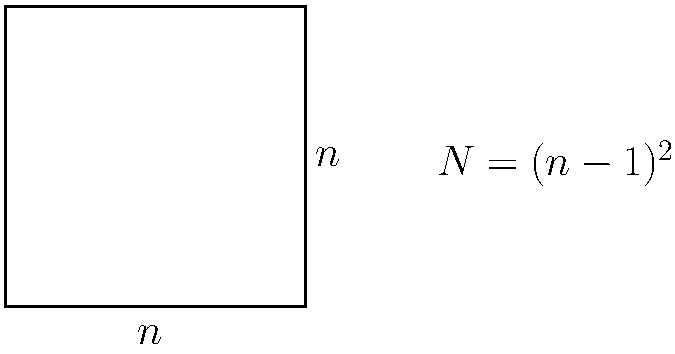
\includegraphics[width=8cm]{Domain2D_ntimesn}
\end{figure}

\begin{align*}
  \tau^n &= \text{ total simulation time (in seconds)} \\
  \tau_1^n &= \frac{\tau}{n^2}
\end{align*}

\begin{table}[h]
  \begin{center}
    \begin{tabular}{|r|l|l|l|}
      \hline
      $n$ & $\tau^n$ & $\tau_1^n$ & $\tau_1^n (m \times m)$ \\
      \hline
      $32$ & $2.36 \cdot 10^{-2}$ & $2.31 \cdot 10^{-5}$ & $1.76 \cdot 10^{-5}$ \\
      $64$ & $1.11 \cdot 10^{-1}$ & $2.71 \cdot 10^{-5}$ & $3.66 \cdot 10^{-5}$ \\
      $128$ & $5.19 \cdot 10^{-1}$ & $3.17 \cdot 10^{-5}$ & $7.34 \cdot 10^{-5}$ \\
      $256$ & $2.35$ & $3.58 \cdot 10^{-5}$ & $1.50 \cdot 10^{-4}$ \\
      $512$ & $10.5$ & $3.99 \cdot 10^{-5}$ & $3.96 \cdot 10^{-4}$ \\
      $1024$ & $46.2$ & $4.41 \cdot 10^{-5}$ & $8.33 \cdot 10^{-4}$ \\
      \hline
      & $\tau^n \sim \mathcal{O}(n^2 \log n)$ & $\tau_1^n \sim \mathcal{O}(\log n)$ & $\tau_1^n \sim \mathcal{O}(n) $ \\
      \hline
    \end{tabular}
  \end{center}
  \caption{Simulation results for the numerical approximation of the two-dimensional Poisson equation by the use of fast diagonalization techniques.}
\end{table}

\newpage
\begin{verbatim}
      program poisson
c==================================================================
c
c     FORTRAN-program to solve the two-dimensional Poisson equation
c     on a unit square using finite differences (five-point stencil),
c     one-dimensional eigenvalue decompositions and fast sine transforms.
c     In this example, the right hand side f=1.
c
c     note: n needs to be a power of 2
c
c     einar m. ronquist
c     ntnu, october 2000
c
c===================================================================
      parameter (n  = 256)
      parameter (m  = n-1)
      parameter (nn = 4*n)
c
      real*8    diag(m), b(m,m), bt(m,m)
      real*8    pi
      real*8    z(0:nn-1)
      real*4    tarray(2), t1, t2, dt

      h    = 1./n
      pi   = 4.*datan(1.)

      do i=1,m
         diag(i) = 2*(1-dcos(i*pi/n))
      enddo

      do j=1,m
         do i=1,m
            b(i,j) = h*h
         enddo
      enddo

      \end{verbatim}
      \newpage
      \begin{verbatim}
      do j=1,m
         call fst (b(1,j), n, z, nn)
      enddo
      call transp (bt, b, m)
      do i=1,m
         call fstinv (bt(1,i), n, z, nn)
      enddo


      do j=1,m
         do i=1,m
            bt(i,j) = bt(i,j)/(diag(i)+diag(j))
         enddo
      enddo


      do i=1,m
         call fst (bt(1,i), n, z, nn)
      enddo
      call transp (b, bt, m)
      do j=1,m
         call fstinv (b(1,j), n, z, nn)
      enddo



      umax = 0.0
      do j=1,m
         do i=1,m
            if (b(i,j) .gt. umax) umax = b(i,j)
         enddo
      enddo

      write(6,*) ' '
      write(6,*) umax

      stop
      end

\end{verbatim}
\newpage
\begin{verbatim}

      subroutine transp (at, a, m)
c====================================================
c     set at equal to the transpose of a
c====================================================
      real*8 a(m,m), at(m,m)

      do j=1,m
         do i=1,m
            at(j,i) = a(i,j)
         enddo
      enddo
      return
      end



\end{verbatim}

\lstset{inputpath=code/mpiio/}

\chapter{Parallel I/O in MPI}

\section{Introduction}

As HPC applications grow larger and larger as more and more computing resources
are made available, so does the volume of data which needs to be handled, both
on the input and the output side of the application. The process of reading data
into a process or storing data from a process we hereby refer to as \emph{I/O}.
The input side is mostly a solved problem, in the sense that most operating
systems and filesystems added support for multiple processes reading from the
same file years ago.

\begin{figure}
  \centering
  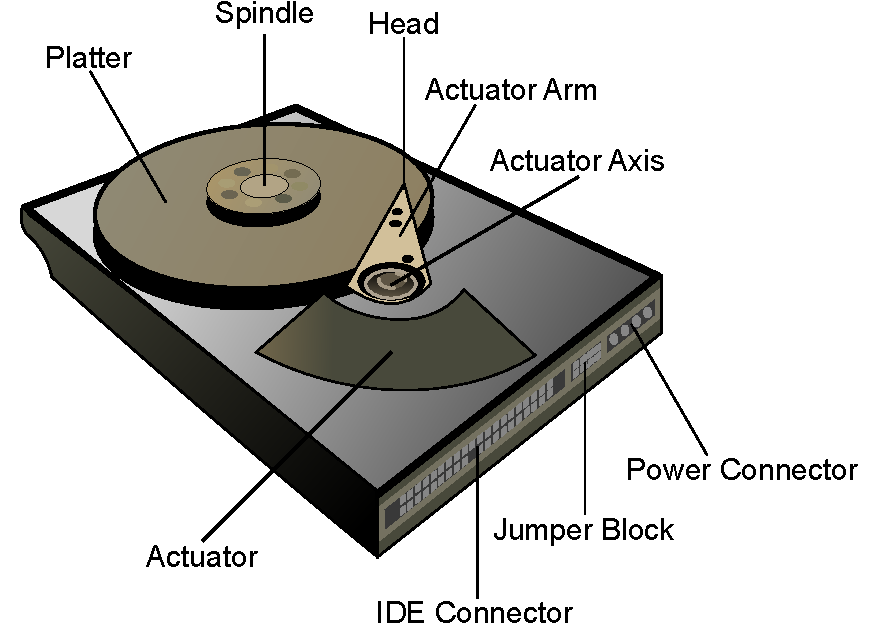
\includegraphics[width=12cm]{Hard_drive-en}
  \caption{
    Illustration of the interior of a hard disk drive. The data is stored on
    platters. The data is stored magnetically on these platters by a magnetic
    device referred to as the \emph{head}. The same device is responsible for
    retrieving the data when a read operation is issued. Since we only have a
    single head, HDDs are serial by construction. Image taken from
    \url{http://en.wikipedia.org/wiki/Harddrive}.
  }
  \label{fig:hdd}
\end{figure}

Getting high performance, however, is more involved. For the last thirty years
or so, secondary storage has usually been hard disk drives (commonly abbrevated
as \emph{HDDs}); see \autoref{fig:hdd} for an illustration of the interior.
These are mechanical in nature, data is read/written from/to spinning platters
through a magnetic device referred to as the \emph{head}. Since a HDD only has a
single head, it can only perform a single read/write operation concurrently.
This means that even though multiple processes can initiate reads concurrently,
they will be performed in serial. Schematically this can be illustrated as in
\autoref{fig:manyone}. A HDD only performs at peak levels if data is read or
written in large sequential chunks, since searching for data incur large
penalties, as the head has to be repositioned. In a lot of HPC applications, the
access pattern for a single process can seem to be fairly random from the
operating system's point of view, which lead to the I/O being performed in an
inefficient manner. This is due to the fact that the data a particular process
needs is scattered in the file, leading to excessive seeks. Only when all the
I/O performed by the separate processes are considered as a whole, a sequential
pattern can be found. The application developer is often aware of this fact, and
this raises the need for an interface where this information can be given to the
system. Additional performance can be achieved if a file is stored across
multiple storage devices. This allows us to harness the aggregated bandwith of
the devices; see \autoref{fig:manymany} for an illustration.

\begin{figure}
  \begin{center}
    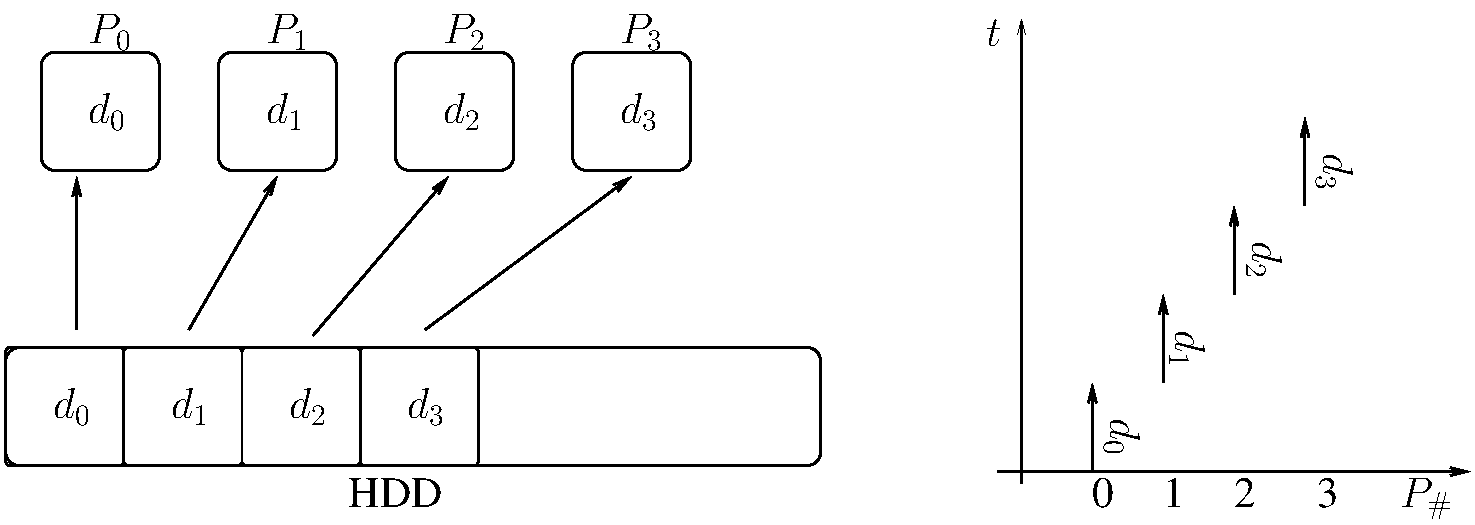
\includegraphics[width=12cm]{many-onedisk}
  \end{center}
  \caption{
    Illustration of I/O where several processes read from a single file. Since a
    HDD is serial in nature, only one operation can be performed concurrently.
  }
  \label{fig:manyone}
\end{figure}
\begin{figure}
  \begin{center}
    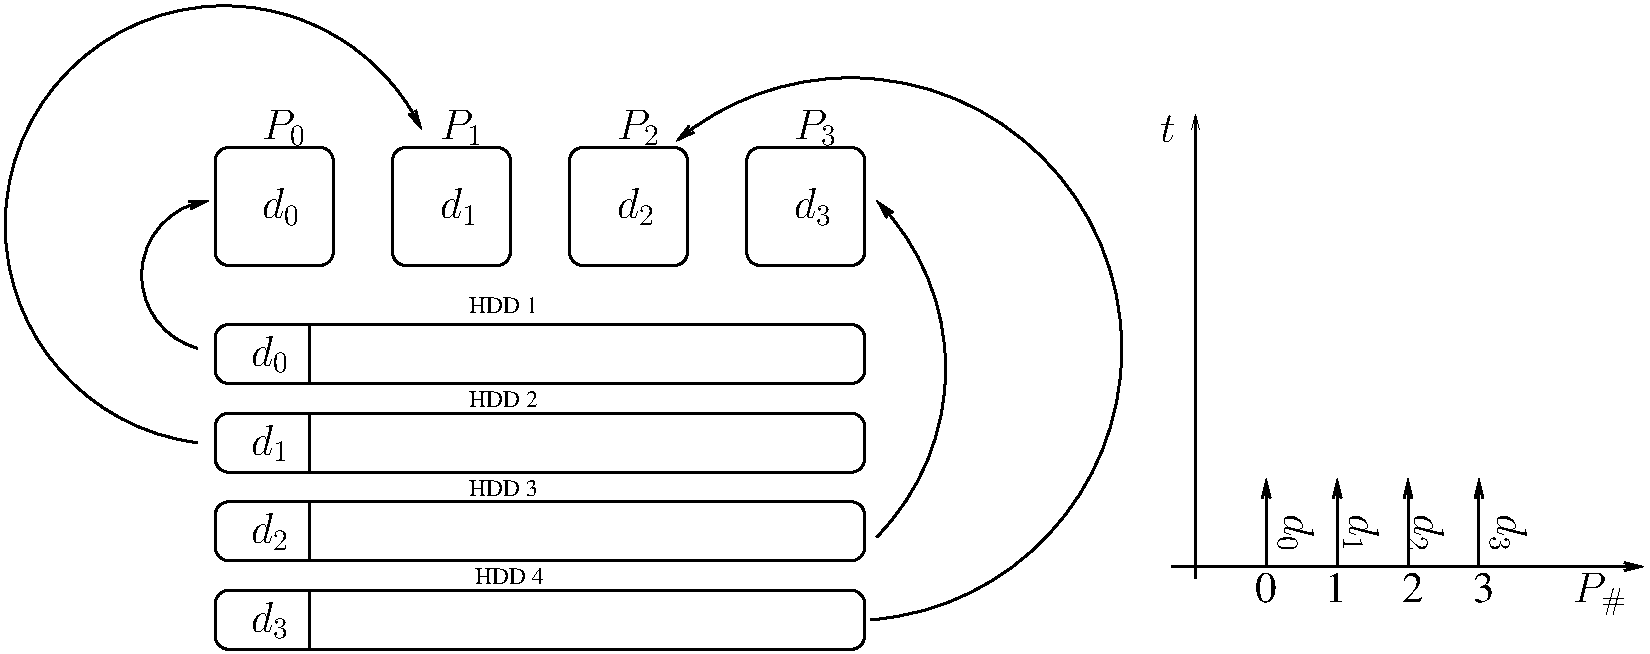
\includegraphics[width=12cm]{many-manydisk}
  \end{center}
  \caption{
    Illustration of I/O where we harness the aggregated bandwith of several
    devices. Here each process reads its data from a separate physical device,
    thus the I/O can be performed in parallel.
  }
  \label{fig:manymany}
\end{figure}

On the output side, things turn are interesting. For years HPC applications
solved their needs using one of two approaches. The first approach is often
referred to as \emph{post-mortem assembly}; each process dumps its data to a
separate file, and then custom-tailored code is used to read the data into the
next application in the computational chain, such as visualization software. If
implementing the support directly into the visualization software is not
feasible, a separate postprocessing application must be written. The second
approach, which is also often used, is to serialize the I/O. Here one process is
given the responsibility of writing the data to disc. The other processes then
simply send their data to the responsible process, in a sequential manner; see
\autoref{fig:serial}.

\begin{figure}
  \begin{center}
    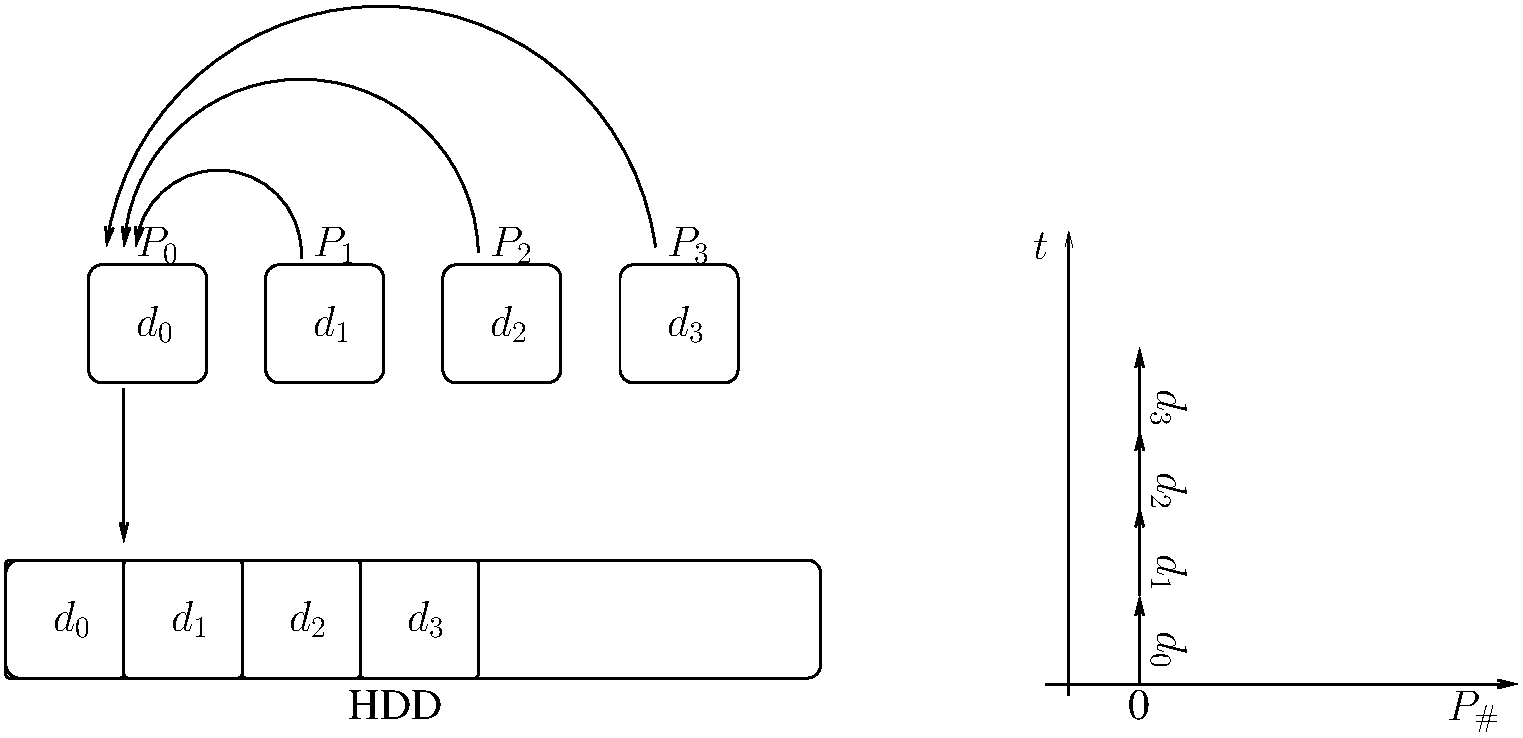
\includegraphics[width=12cm]{serial}
  \end{center}
  \caption{
    Illustration of serialization of the I/O. All processes send their data to
    process 0, which is responsible for writing the data to secondary storage.
    Since a harddrive is serial in nature, the total time spent on the operation
    equals the sum of the time to write the individual data chunks.
  }
  \label{fig:serial}
\end{figure}

What is common to both of these approaches, is that they necessitate performing
(most of) the I/O in a serial manner. As the data volume grows, this occupies an
increasing amount of the total computational time. Eventually this may become a
large bottleneck for the parallel performance of your program. The first
approach also necessitates performing substantially more I/O than strictly
required, in particular all data is written twice; first to the separate files
and then in a stitched-together fashion as performed by the postprocessing
application. If the volume of data is substantial, this introduces another
severe bottleneck in your computational chain. The code involved in both of
these approaches is often intricate and prone to errors.

It is thus of great interest to be able to store all data in a single file, or
at most a few files, while avoiding serialization of the I/O both on the
application level, as well as on the physical level, by splitting the file
across multiple storage devices. Fortunately there are established libraries to
enable this. We here consider one particular example of such an interface,
namely the \emph{MPI-IO} interface. As the name implies, this was made part of
the official MPI standard back in 1998 with the introduction of the MPI 2.0
specification. However, while the library strive to yield highly portable code,
tuning to the underlying filesystem (how the data is stored on the hard disk
drive(s)) is unavoidable when it comes to obtaining high performance. One
example of such a file system is the \emph{general parallel filesystem}, GPFS
for short, developed by IBM during the last 10 years. This is in use on NOTUR
systems (\emph{Kongull}, \emph{Vilje}). Since such tuning is somewhat technical
and beyond the intention of this document, this will not be discussed in detail
in the following.

\section{Basic concepts of MPI-IO}

MPI-IO is the part of the official MPI standard which covers parallel I/O. It
offers a simple, natural interface for expressing parallelism in I/O. Informing
the system about the underlying distributed nature of an I/O call enables the
system to make good choices about how the I/O is performed on a lower level. We
first consider the simplest case: I/O that is sequential on each process.

\subsection{Sequential I/O}

We here consider sequential I/O, namely writing a contiguous slice of data from
a set of separate processes. The data storage pattern in this case is fairly
trivial, as illustrated in \autoref{fig:contigousstorage}. An example where such
a pattern could occur, is if we have partitioned a matrix in a strip fashion
across the processes; see \autoref{fig:strip} for an illustration.

\begin{figure}[ht]
  \begin{center}
    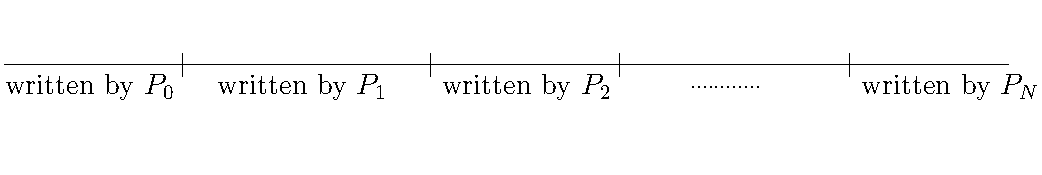
\includegraphics[width=12cm]{slicedvector}
  \end{center}
  \caption{
    Illustration of an I/O operation where a contiguous piece of data is sliced
    into chunks. A single contiguous chunk of data is then written by each
    process. All the chunks are written to the same file.
  }
  \label{fig:contigousstorage}
\end{figure}

If you are familiar with standard POSIX I/O calls, the basic form of
the MPI-IO code should look very familiar. On each process we start by
opening a handle to the file we want to write to, in this case called
``datafile''.
\lstinputlisting[style=c]{open-handle.c}
A file handle is described by a variable of type \texttt{MPI\_File}. In addition
to which file we want to open, we also have to specify flags which the system
use to both control which accesses are allowed, as well as for directives which
help increase performance. Here we only specify flags of the former class, in
particular, we only want to write to the file (by specifying the flag
\texttt{MPI\_MODE\_WRONLY}) and we want the file to be created if it doesn't
already exist (by specifying the flag \texttt{MPI\_MODE\_CREATE}). The function
includes an additional parameter of type \texttt{MPI\_Info}. For now we pass the
builtin value \texttt{MPI\_INFO\_NULL} which can be used when we do not want to
pass any data in this field. We will briefly comment on this later.

With the file opened, we proceed with writing the data. In this example, our
data is an array of doubles named \texttt{vec}. The total global array length is
\texttt{N}, which means we have \texttt{N/size} elements per process (here
\texttt{size}, as usual, denotes the number of processes, while \texttt{rank}
denotes the process number). We first seek to the appropriate offset in the
file, then write the chunk of data.
\lstinputlisting[style=c]{separate-handle-write.c}

An alternative way of doing the same operation, is to use the \emph{explicit
offset} \texttt{MPI\_File\_Write\_at} function. This is mainly a matter of
convenience, i.e. it allows to do the same operation with less code, in
particular, we avoid the seek call;
\lstinputlisting[style=c]{explicit-offset-write.c}

Common to both of these alternatives is that they use individual I/O calls on
each process. If the underlying system is smart, it should be able to recognize
the access pattern. If we want to make sure that the system notices this fact,
we can use \emph{collective} calls. In particular, consider
\lstinputlisting[style=c]{collective-write.c}
Here we inform the system that we are performing a collective write among all
the processes. This allows the system to do additional coordination of how the
I/O is performed. However, it comes at a cost. In particular, all processes will
stall until the entire I/O operation is completed across all the processes,
while using individual handles allows the program flow to continue on each
process as soon as their share of the I/O has been performed.

Another convenience function in the context of collective calls is \emph{shared}
writes. In addition to containing info about the position on the individual
processes, a \texttt{MPI\_File} variable also contains info about a shared state
between all the processes. Here, with our simple data layout, this can be
exploited to make the code particularly simple. We simply have to do
\lstinputlisting[style=c]{shared-write.c}
This function uses the shared state in the file pointer. Upon the call, the writes
are performed in order according to process rank.

Finally we have to close our file. This is performed by doing
\lstinputlisting[style=c]{close.c}

\section{Non-sequential I/O: file views}

In the previous section we considered an extremely simple data access pattern.
Such a pattern is only the predominant one in simple codes. Usually the access
patterns in real applications are much more involved. Programming such access
patterns naively using many seeks and many small writes is certainly a
possibility, however hardly something we would recommend. In addition to being
highly error prone, it would also make it very hard for the system to get a
proper view of the collective I/O performed across the processes.

For purposes of easy presentation, we here again consider a simple data layout.
In particular, consider a vector split in a cyclic manner, see
\autoref{fig:cyclicvector}.

\begin{figure}
  \begin{center}
    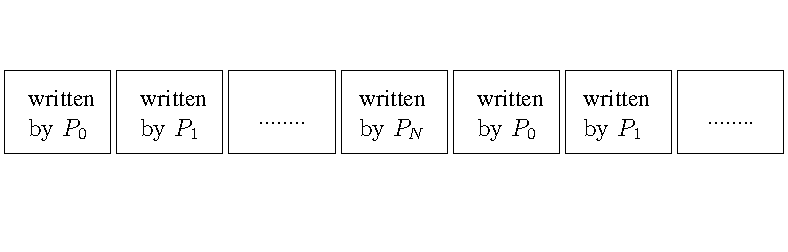
\includegraphics[width=12cm]{splitvector}
  \end{center}
  \caption{
    Illustration of cyclic partition of a vector. Each process writes a single
    number, followed by a gap of $\text{size}-1$ numbers. This pattern repeats for the
    extent of the data.
  }
  \label{fig:cyclicvector}
\end{figure}

If we perform this I/O naively, each process would write a single number,
perform a seek, write another number and so on. Such small writes followed by
seeks makes it very hard for the system to optimize the I/O. MPI-IO offers a
much better approach. It builds on the MPI machinery for constructing custom
types. While these datatypes are used to describe the data layout in memory in
standard MPI functions, they are here used to describe the data layout on
secondary storage. From each process, the data access pattern is one number
followed by a gap of $\text{size}-1$ numbers. We can describe such a pattern in
a MPI datatype as
\lstinputlisting[style=c]{createsplitview.c}
We here use the function
\begin{lstlisting}[style=c]
  MPI_Type_create_resized(origtype, lb, extent, newtype)
\end{lstlisting}
to create the gap. We set \texttt{lb} (lower bound) = 0 to indicate that we want
the real data to start at the beginning of the new data type. We then extend
this to be size doubles long. We can now attach this view of the data to the
file using the function
\begin{lstlisting}[style=c]
  MPI_File_set_view(fh, disp, datatype,
                    viewtype, encoding, info)
\end{lstlisting}
as
\lstinputlisting[style=c]{setsplitview.c}
Note the usage of the \emph{disp} field. This field describes an offset that the
process sees as the start of the file. By setting this offset equal to position
of the first number the particular process should write to the file, the
data access pattern (\emph{MPI\_Datatype}) we described further up is exactly
the same on each process. With this configured, writing the data to the file in
the proper pattern is now just a normal write call, e.g. using separate handles
\lstinputlisting[language=C]{writesplitview.c}
A code demonstrating this can be found in Appendix \ref{app:cyclicvector}.

We stress that there is nothing stopping you from using different fileviews on
the different processes. In fact, we now move on to consider a particular case
where this is needed, namely when we want to handle arrays/matrices partitioned
over several processes.

\begin{figure}
  \begin{subfigure}{6cm}
    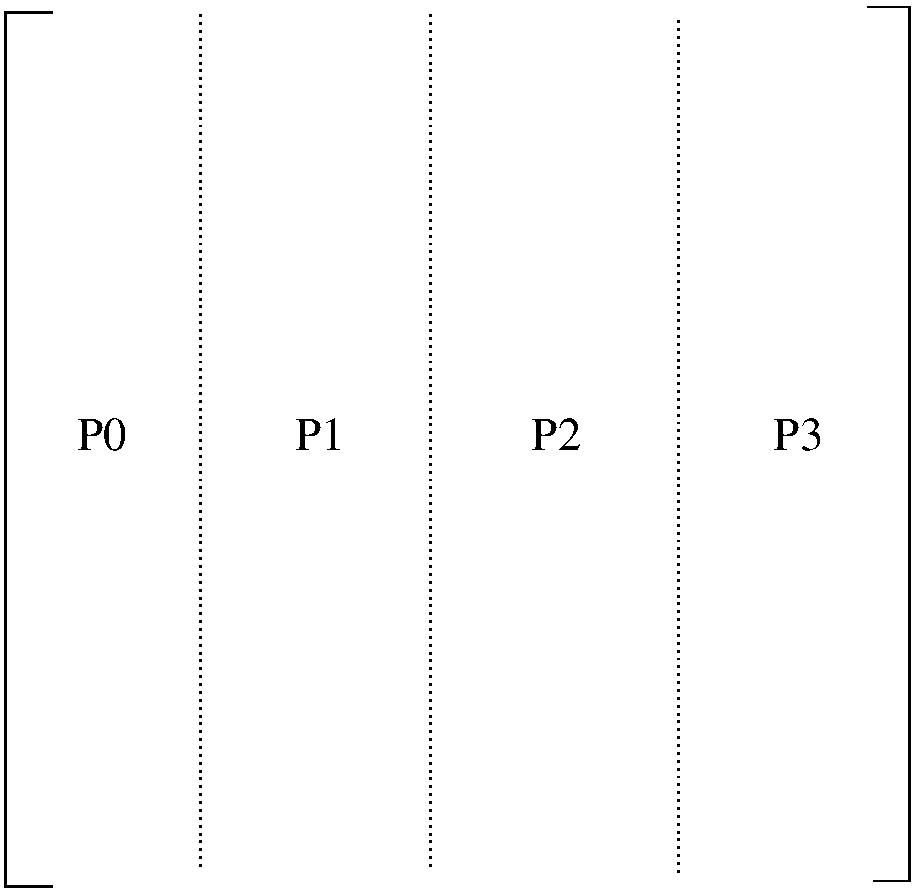
\includegraphics[width=6cm]{strip}
    \caption{Strips.}
    \label{fig:strip}
  \end{subfigure}
  \begin{subfigure}{6cm}
    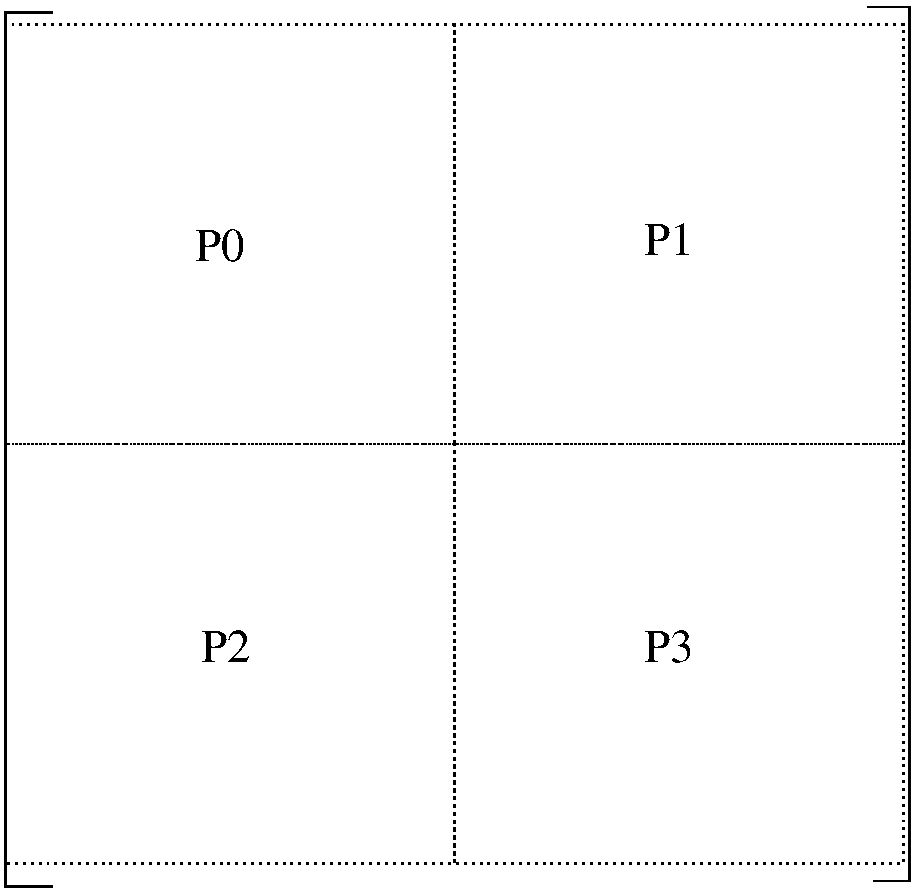
\includegraphics[width=6cm]{block}
    \caption{Blocks.}
    \label{fig:block}
  \end{subfigure}
  \caption{
    Illustration of two possible ways a 2D array can be distributed across
    several processes. In \autoref{fig:strip} each process is responsible for a
    number of whole columns. In \autoref{fig:block} each process is instead
    reponsible for a sub-block of the array.
  }
  \label{fig:darrays}
\end{figure}

\section{Non-sequential I/O: distributed arrays}

In HPC applications, your data usually consists of matrices (2D arrays) or 3D
arrays. This fact has not gone past the MPI creators, and as such MPI contains
machinery for generating partioning of such arrays in a semi-automatic way.
Since MPI-IO is built on MPI, this machinery is also extremely useful when we
want to write the data to secondary storage. We now show how to employ these
utility functions to make writing distributed arrays to disc as simple as
performing a single write call.

MPI names such distributed arrays \emph{darray} for short. The available
functions are heavily inspired by the High Performance Fortran standard, HPF for
short. This is a standard which aims to make developing HPC software easier
through semi-automatic parallelization. In this context, the most important
parts of this standard is its conventions for array partitioning strategies and
process topologies, since MPI follows the same conventions. The two possible
partitionings of most interest in this context is illustrated in
\autoref{fig:darrays}. As we will show shortly, these are to some extent
similar.

\begin{figure}
  \begin{center}
    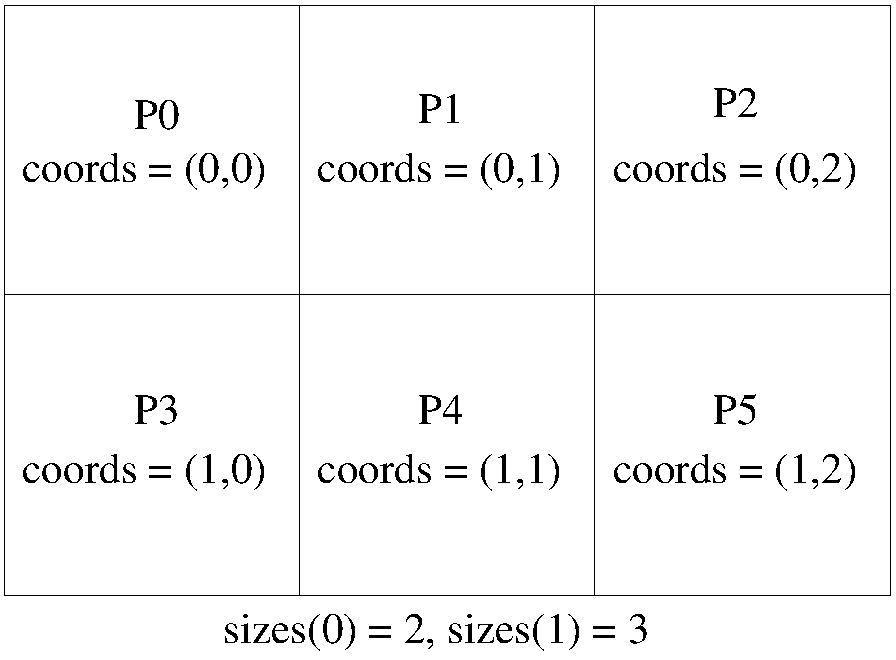
\includegraphics[width=12cm]{splitdomain}
  \end{center}
  \caption{
    A block partition of a 2D array with the pieces of information we need to
    classify this partitioning.
  }
  \label{fig:splitdomain}
\end{figure}

We now show how to use the MPI machinery to easily partition an array. Consider
\autoref{fig:splitdomain}. We here have a 2D array we want to partition across 6
MPI processes. The figure contains the pieces of information we need to classify
a partitioning:
\begin{itemize}
\item A global topology: here a Cartesian topology expressed as the number
  of processes along each dimension (here 2 and 3, respectively).
\item Location of a particular domain in the topology, again
  this can be expressed as an integer along each dimension.
\item A mapping of the available processes onto the topology.
\end{itemize}

The first useful function is \texttt{MPI\_Dims\_create}. This function generates
a Cartesian partioning of your processes according to a the rules set by
HPF.
\lstinputlisting[style=c]{dimsblock.c}
The initialization of the entries in sizes prior to calling the function is
important. In particular, the function will only operate along a dimension $i$
where \texttt{sizes[i] = 0} on function entry. While this interface makes it
very easy for the programmer to make errors (i.e. forgetting to initialize the
array properly), it also has advantages. For instance, if we instead want to
divide our matrix in a strip fashion, we can do
\lstinputlisting[style=c]{dimsstrip.c}
Of course, if we only have one partitioned dimension in our array, generating
the topology is trivial. The nice thing with doing it like this is that it
allows us to use fairly similar code, whether we want a strip or a block
partitioning of the arrays; see \autoref{fig:darrays}. We stress that this only
generates the \emph{topology} (or partitioning structure), it does not in any
way depend on the array dimensions. Upon return from the function the
\texttt{dims} array contains the number of processes used in the separate
directions, 2 and 3, respectively, in our example.

Now we have a topology describing the layout of our processors, or rather how
many processors the dimensions are split over. Still, each processor needs to
know where they are located in this topology. To be able to decide this, we
first have to create a communicator group which has the (Cartesian) topology
attached. This can be achieved by
\lstinputlisting[style=c]{comm.c}
The \texttt{periodic} array is an integer array with either 0 or 1 as entries.
These are used to specify whether or not the domain is periodic in the
particular dimension, which is not the case with a standard 2D array as the one
we consider here. Upon return from the function, the \texttt{comm} variable
holds the new communicator info. This can now be used wherever MPI expects a
communicator (i.e. instead of the builtin \texttt{MPI\_COMM\_WORLD} we have used
previously). This takes care of mapping the processes onto the topology.

Finally, each process can then find their location in the topology using
\lstinputlisting[style=c]{coord.c}
Upon return from the function, the \texttt{coords} array holds the coordinates.
In our example, it would for instance hold 1 and 2 when called on process 5.

With the problem partitioning taken care of, it is time to tie this into MPI-IO.
MPI includes functions to describe such a distributed array layout in memory,
which usually are useful when you want to collect a whole array on a single
process. Collecting all data on a single process is exactly what we want to
perform when we write this to secondary storage, the only difference is that in
our case this ``process'' is the file on secondary storage. Thus we can use the
functions originally intended for describing the data layout in memory to
instead generate the fileviews on the separate processes. The function we need
is
\begin{lstlisting}[style=c]
  MPI_Type_create_darray(size, rank, dims, gsizes,
                         distribs, dargs, sizes,
                         order, etype, newtype)
\end{lstlisting}
Here \texttt{size} is the size of the communicator (typically the number of
processes), \texttt{rank} the process rank within the communicator,
\texttt{dims} the number of dimensions in the array (2 for a matrix),
\texttt{gsizes} the sizes of the global array along the dimensions,
\texttt{distribs} distribution strategies along the dimensions, \texttt{dargs} a
distribution strategy parameter (can usually be set to
\texttt{MPI\_DISTRIBUTE\_DFLT\_DARG}), \texttt{dims} the topology results as
obtained using \texttt{MPI\_Dims\_create}, \texttt{order} describes the array
layout in memory (\texttt{MPI\_ORDER\_C} or \texttt{MPI\_ORDER\_FORTRAN}),
\texttt{etype} the datatype of the array entries and finally \texttt{newtype}
our new datatype.

The most interesting of these are the \texttt{distribs} array. This array
contains the chosen distribution strategy along each dimension. The strategy can
be one of
\begin{itemize}
\item \texttt{MPI\_DISTRIBUTE\_NONE}: Here no partitioning of the array is applied along
  this dimension.
\item \texttt{MPI\_DISTRIBUTE\_CYCLIC}: Here a cyclic partitioning of the array is applied
  along this dimension. This distribution is often used in HPF codes. We do not
  consider it here.
\item \texttt{MPI\_DISTRIBUTE\_BLOCK}: Here a block partitioning of the array is applied
  along this dimension.
\end{itemize}
For instance, if we want to block-partition an array of doubles with size
$N\times N$ stored according to C convections (row-major storage), we do
\lstinputlisting[style=c]{createarrayview.c}
If we now set this datatype as the fileview on the individual processes as
described earlier, we can now write them to disc using a single write call. This
is much much easier than the alternative using separate write/seek calls.

A code that handles both strip and block partitioned arrays can be found in
Appendix \ref{app:darray}.

\section{Overlapping I/O and computations}

On modern architectures HDDs can write/read data (almost) completely on their
own using a technique known as \emph{Direct Memory Access}, \emph{DMA} for
short. This means that while we are writing/reading data the CPU is mostly an
idle observer. This is not good for program efficiency, ideally we would like to
keep the CPUs saturated with work whenever we can. MPI-IO also offers facilities
to remedy this, namely \emph{non-blocking} I/O. All classes of I/O calls have
non-blocking equivalents, to simplify the presentation we here only consider
using individual handles on each process.

The basic idea can be summarized in the following piece of (somewhat) abstract
code;
\lstinputlisting[style=c]{overlapping.c}
We have here replaced the \texttt{MPI\_File\_write} function with a call to
\texttt{MPI\_File\_iwrite}, which is the nonblocking equivalent. This call
initiates the I/O operation, then immediately returns. The function takes an
additional parameter of type \texttt{MPI\_Request}. Upon the return from the
function call, this will be updated with information which identifies the I/O
operation. We are now free to perform additional calculations, as long as the
data we just requested written to secondary storage is not touched by this code.
In particular, the vector \texttt{vec} cannot be updated in the
\texttt{doSomething()} call. When we get to a point where we need write access
to the vector \texttt{vec} again, we do a call to \texttt{MPI\_Wait} with the
\texttt{MPI\_Request} variable as a parameter. This function will only return
once it is safe to reuse \texttt{vec}. Note that a call to a nonblocking I/O
function \emph{ALWAYS} needs to be accompanied with a call to
\texttt{MPI\_Wait}, even if you do not plan to reuse the memory area you
requested written to secondary storage.

\section{Tuning for performance}

As mentioned in the introduction, a program using MPI-IO needs to be tuned to
the particular underlying filesystem if we want the best performance. This
tuning can be divided in two classes.

\begin{itemize}
\item \textbf{Directives}: This class of tuning parameters are something an
  implementation has to obey. One example of such a tuning parameter is the flag
  \texttt{MPI\_MODE\_SEQUENTIAL} which can be passed upon opening the file, just
  like we passed e.g. \texttt{MPI\_MODE\_WRONLY} earlier. This tells the system
  that only sequential access to the data is performed, information which can be
  used to optimze the I/O.
\item \textbf{Hints}: These are, as the name indicates, just hints to the
  implementation. If an implementation does not support/utilize a particular
  hint, they can just be silently ignored. This is the framework in which vendor
  specific/filesystem specific tuning can be performed.
\end{itemize}

These hints are passed to the implementation in a variable of type
\texttt{MPI\_Info}. First we need to create the appropriate structure, this is
achieved through
\lstinputlisting[style=c]{infoinit.c}
We can now set hints in this structure. A hint is a pair of (key,value) strings.
We add such a hint to our \texttt{MPI\_Info} variable using the function
\begin{lstlisting}[style=c]
  MPI_Info_set(info, key, value)
\end{lstlisting}
Such a call might look like
\lstinputlisting[style=c]{infoset.c}

Once we have added all hints we want to the \texttt{MPI\_Info} variable, we can
now pass these hints to the implementation upon opening a file.
\lstinputlisting[style=c]{infoopen.c}
We here pass our \texttt{MPI\_Info} variable instead of \texttt{MPI\_INFO\_NULL}
as earlier.

\section{Further reading}
You can find the MPI-IO standard as well as tutorials on the official
MPI homepage \url{http://www.mpi-forum.org/}. Some useful papers and slides
can be found at
\url{https://computing.llnl.gov/?set=code\&page=sio\_papers\_presentations}.
These are of particular interest if you want extensive knowledge about using
MPI-IO on top of GPFS.

\textbf{Acknowledgements}: J{\o}rn Amundsen gave some useful pointers while this
chapter was written, in particular the link to \url{llnl.gov}. Tobias Arrskog
helped with proof reading. The chapter was written by Arne Morten Kvarving. Your
assistance was greatly appreciated.


\nocite{openmp}
\nocite{openmptut}
\nocite{towards}
\nocite{mpi-io}
\nocite{mpi-io2}
\nocite{culler1999parallel}
\nocite{douglas2000portable}
\nocite{lande2004}

\bibliographystyle{plain}
\bibliography{references}

\appendix

\chapter{OpenMP code}
\lstset{inputpath=code/openmp/}

\section{Calculating $\pi$ with an integral in OpenMP}
\label{app:openmp-integrate}
\lstinputlisting[style=c]{serial.c}

\chapter{MPI-IO code}
\lstset{inputpath=code/mpiio/}

\section{Storage of a cyclic-partitioned vector using MPI-IO}
\label{app:cyclicvector}
\lstinputlisting[style=c]{fileview.c}

\newpage

\section{Storage of a block/strip partitioned array using MPI-IO}
\label{app:darray}
\lstinputlisting[style=c]{combined.c}

\end{document}
